\documentclass{dissertation}
%\documentclass[print]{dissertation}  %%%%%%%%%%%%%%%%%%%%%%%%%%%%%%%% CHECK
%\documentclass[print,draft]{dissertation}

\usepackage{booktabs}
\usepackage{graphicx}
\usepackage{arydshln}
\usepackage{wrapfig}
\usepackage{acronym}
\usepackage{caption}
\usepackage[font=footnotesize]{subcaption}
\usepackage{hhline}
\usepackage{tcolorbox}
\usepackage{pdfpages}

\usepackage{qrcode}
\usepackage{enumitem}

\Crefname{section}{Sec.}{Secs.}
\Crefname{section}{Section}{Sections}
\Crefname{table}{Table}{Tables}
\Crefname{table}{Tab.}{Tabs.}

\newcommand{\chapref}[1]{Chapter~\ref{#1}}
\newcommand{\chapreftwo}[2]{Chapters~\ref{#1} and~\ref{#2}}
\newcommand{\chaprefthree}[3]{Chapters~\ref{#1},~\ref{#2}, and~\ref{#3}}
\newcommand{\chapreffour}[4]{Chapters~\ref{#1}, \ref{#2}, \ref{#3}, and~\ref{#4}}
\newcommand{\secref}[1]{Section~\ref{#1}}
\newcommand{\appref}[1]{Appendix~\ref{#1}}
\newcommand{\figref}[1]{Fig.~\ref{#1}}
\newcommand{\eqnref}[1]{Eq.~\ref{#1}}
\newcommand{\tabref}[1]{Table~\ref{#1}}
\newcommand{\eqnreftwo}[2]{Eqs.~\ref{#1} and~\ref{#2}}
\newcommand{\secreftwo}[2]{Sections~\ref{#1} and~\ref{#2}}
\newcommand{\figreftwo}[2]{Figs.~\ref{#1} and~\ref{#2}}
\newcommand{\figrefthree}[3]{Figs.~\ref{#1}, {#2} and~\ref{#3}}
\newcommand{\tabreftwo}[2]{Tables~\ref{#1} and~\ref{#2}}
\newcommand{\R}{\mathbb{R}}
\newcommand{\mli}[1]{\mathit{#1}}
\providecommand{\e}[1]{\ensuremath{\times 10^{#1}}}
\newcommand{\norm}[1]{\left\lVert#1\right\rVert}

\makeatletter
\def\thickhline{%
	\noalign{\ifnum0=`}\fi\hrule \@height \thickarrayrulewidth \futurelet
	\reserved@a\@xthickhline}
\def\@xthickhline{\ifx\reserved@a\thickhline
	\vskip\doublerulesep
	\vskip-\thickarrayrulewidth
	\fi
	\ifnum0=`{\fi}}
\makeatother

\newlength{\thickarrayrulewidth}
\setlength{\thickarrayrulewidth}{2\arrayrulewidth}

\newenvironment{blockquote}{%
	\par%
	\leftskip=2em\rightskip=2em%
	\noindent\ignorespaces}{%
	\par
}

\renewcommand*{\UrlFont}{\color{tudelft-orange}\relax}  %%%%%%%%%%%%%%%%%%%%%% CHANGE
\begin{document}
	\title{Self-Supervised Neuromorphic Perception\\\vspace{5pt} for Autonomous Flying Robots}
	\author{Federico}{Paredes-Vallés}
	
	% REMOVE FOR PRINTING
	\setcounter{page}{0}\includepdf[pages=-]{coverfront.pdf}  %%%%%%%%%%%%%%%%%%%%%%%%%%%%%%%% CHECK
	
	%%%%%%%%%%%%%%%%%%%%%%%%%
	\frontmatter
	
	% cover width: 5+170+15(prob)+170+5 = 365
	% cover height: 5+240+5 = 250
	\begin{titlepage}

\begin{center}

%% Extra whitespace at the top.
\vspace*{2\bigskipamount}

%% Print the title.
{\makeatletter
\titlestyle\bfseries\LARGE\@title
\makeatother}

%% Print the optional subtitle.
{\makeatletter
\ifx\@subtitle\undefined\else
    \bigskip
    \titlefont\titleshape\Large\@subtitle
\fi
\makeatother}

\end{center}

\cleardoublepage
\thispagestyle{empty}

\begin{center}

%% The following lines repeat the previous page exactly.

\vspace*{2\bigskipamount}

%% Print the title.
{\makeatletter
\titlestyle\bfseries\LARGE\@title
\makeatother}

%% Print the optional subtitle.
{\makeatletter
\ifx\@subtitle\undefined\else
    \bigskip
    \titlefont\titleshape\Large\@subtitle
\fi
\makeatother}

%% Uncomment the following lines to insert a vertically centered picture into
%% the title page.
%\vfill
%\includegraphics{title}
\vfill

%% Apart from the names and dates, the following text is dictated by the
%% promotieregelement.

{\Large\titlefont\bfseries Dissertation}

\bigskip
\bigskip

for the purpose of obtaining the degree of doctor

at Delft University of Technology,

by the authority of the Rector Magnificus, prof.~dr.~ir.~T.\ H.\ J.\ J.~van~der~Hagen,

chair of the Board for Doctorates,

to be defended publicly on Friday 24 February 1995 at 10:00 o'clock

\bigskip
\bigskip

by

\bigskip
\bigskip

%% Print the full name of the author.
\makeatletter
{\Large\titlefont\bfseries\@firstname\ {\titleshape\@lastname}}
\makeatother

\bigskip
\bigskip

Master of Science in Aerospace Engineering, \\
Delft University of Technology, The Netherlands,

born in Katwijk, The Netherlands.

%% Extra whitespace at the bottom.
\vspace*{2\bigskipamount}

\end{center}

\clearpage
\thispagestyle{empty}

%% The following line is dictated by the promotieregelement.
\noindent This dissertation has been approved by the promotors.

\bigskip
\noindent Composition of the doctoral committee:

%% List the committee members, starting with the Rector Magnificus and the
%% promotor(s) and ending with the reserve members.
\medskip\noindent
\begin{tabular}{p{4.3cm}l}
Rector Magnificus, & chairman \\
prof.\ dr.\ G.\ C.\ H.\ E.\ de Croon, & Delft University of Technology, promotor \\
prof.\ dr.\ S.\ M.\ Boht\'e, & Centrum Wiskunde \& Informatica, promotor\\  % or UvA?

\medskip
\mbox{\emph{Independent members:}} & \\

prof.\ dr. S.\ M.\ Boht\'e, & Centrum Wiskunde \& Informatica, The Netherlands \\
prof.\ dr.\ ir.\ P.\ Campoy, & Universidad Polit\'ecnica de Madrid, Spain \\
prof. dr.\ ir.\ G.\ Gallego, & Technische Universität Berlin, Germany \\
dr.\ Y.\ Sandamirskaya, & Intel Labs and Zurich University of Applied \\
 & Sciences, Switzerland \\
prof.\ dr.\ ir.\ M.\ Wisse, & Delft University of Technology \\
%prof.\ dr.\ ir.\ M.\ Mulder (reserve), & Delft University of Technology \\
prof.\ dr.\ ir.\ M.\ Mulder, & Delft University of Technology, reserve member\\
\end{tabular}

%% Here you can include the logos of any institute that contributed financially
%% to this dissertation.
\vfill
\begin{center}
\includegraphics[height=0.55in]{01_title/logos/tudelft}
\hspace{2em}
\includegraphics[height=0.55in]{01_title/logos/nwo}
\end{center}
\vfill

\noindent
\begin{tabular}{@{}p{0.2\textwidth}@{}p{0.8\textwidth}}
\textit{Keywords:} & Artificial neural networks; Autonomous drone racing; Deep learning; Event-based cameras; Flying robots; Neuromorphic computing; Optical flow; Self-supervised learning; Spiking neural networks; Unsupervised learning  \\[\medskipamount]
\textit{Printed by:} & Ipskamp Printing, \url{www.ipskampprinting.nl} \\[\medskipamount]
\textit{Cover by:} & J.J. Hagenaars
\end{tabular}

\vspace{4\bigskipamount}

\noindent Copyright \textcopyright\ 2023 by F.~Paredes-Vall\'es

%% Uncomment the following lines if this dissertation is part of the Casimir PhD
%% Series, or a similar research school.
%\medskip
%\noindent Casimir PhD Series, Delft-Leiden 2015-01

\medskip
\noindent ISBN 978-94-6366-755-5

\medskip
\urlstyle{same}
\noindent An electronic version of this dissertation is available at \\
\url{http://repository.tudelft.nl/}.

\end{titlepage}


	\tableofcontents
	\chapter*{Summary}
\addcontentsline{toc}{chapter}{Summary}
\setheader{Summary}

\dropcap{I}{n} the ever-evolving landscape of robotics, the quest for advanced synthetic machines that seamlessly integrate with human lives and society becomes increasingly paramount. At the heart of this pursuit lies the intrinsic need for these machines to perceive, understand, and navigate their surroundings autonomously. Among the senses, vision emerges as a cornerstone of human perception, providing a wealth of information about the world we inhabit. Thus, it comes as no surprise that equipping robots with vision-based perception capabilities, or computer vision, has captivated researchers for decades. Recent breakthroughs, fueled by the advent of deep learning, have propelled computer vision to new heights. However, challenges persist in leveraging the power of deep learning, as its hunger for computational resources poses hurdles in the realm of robotics, particularly for small flying robots with their inherent limitations of payload and power consumption. 

This dissertation embarks on a journey that begins at the intersection of two groundbreaking technologies with the potential to revolutionize computer vision and enhance its accessibility to small robots: event-based cameras and neuromorphic processors. These two technologies draw inspiration from the information processing mechanisms employed by biological brains. Event-based cameras output sparse events encoding pixel-level brightness changes at microsecond resolution, while neuromorphic processors leverage the power of spiking neural networks to realize a sparse and asynchronous processing pipeline.

Throughout this dissertation, comprehensive investigations have been conducted, presenting innovative solutions and advancements in the fields of computer vision and robotics. The thesis begins by presenting the winning solution of the 2019 AIRR autonomous drone racing competition, which showcases a monocular vision-based navigation approach specifically designed to address the limitations of conventional sensing and processing methods. Moreover, it explores the bridging of the gap between event-based and frame-based domains, enabling the application of conventional computer vision algorithms on event-camera data. Building upon these achievements, the thesis introduces a pioneering spiking architecture that enables the estimation of event-based optical flow, with emergent selectivity to local and global motion through unsupervised learning. Additionally, the thesis presents a framework that addresses the practicality and deployability of the models by training spiking neural networks to estimate low-latency, event-based optical flow with self-supervised learning. Finally, this dissertation culminates with a demonstration of the integration of neuromorphic computing in autonomous flight. By utilizing an event-based camera and neuromorphic processor in the control loop of a small flying robot for optical-flow-based navigation, this research showcases the practical implementation of neuromorphic systems in real-world scenarios. Overall, our studies demonstrate the benefits of incorporating neuromorphic technology into the vision-based state estimation pipeline of autonomous flying robots, paving the way for the development of more power-efficient and faster neuromorphic vision systems.
	\chapter*{Acronyms}
\addcontentsline{toc}{chapter}{Acronyms}
\setheader{Acronyms}


%--- Acronyms -----------------------------------------------------------------%
% \acrodef{label}[acronym]{written out form} % acronym syntax
%\acrodef{etacar}[$\eta$ Car]{Eta Carinae}   % acronym example
%--- Acronyms -----------------------------------------------------------------%
% how to use acronyms:
% \ac = use acronym, first time write both, full name and acronym
% \acf = use full name (text + acronym)
% \acs = only use acronym
% \acl = only use long text
% \acp, acfp, acsp, aclp = use plural form for acronym (append 's')
% \acsu, aclu = write + mark as used
% \acfi = write full name in italics and acronym in normal style
% \acused = mark acronym as used
% \acfip = full, emphasized, plural, used
%--- Acronyms -----------------------------------------------------------------%

\noindent
\begin{longtable}{p{.225\textwidth} p{.70\textwidth}}
\end{longtable}

	
	%%%%%%%%%%%%%%%%%%%%%%%%%
	\mainmatter
	\thumbtrue
	
	\chapter{Introduction}\label{cha:intro}

\dropcap{F}{lying} insects perform remarkable feats of agile navigation with brains containing less than a million neurons and consuming mere microwatts of power. A honeybee can hover, avoid obstacles, and land on flowers while processing visual information at microsecond timescales---all with a brain smaller than a grain of rice~\cite{decroon2022insectinspired}. In contrast, modern autonomous flying robots typically require tens of watts of power and hundreds of grams of computational hardware to achieve even basic autonomous flight~\cite{nvidia}. This stark difference suggests that current approaches to robot vision may be fundamentally misaligned with the constraints faced by highly resource-limited platforms. The question then becomes: can we rethink robot vision from the ground up to better match the sparse, asynchronous, and energy-efficient principles exhibited by biological systems?

Over the past decade, deep artificial neural networks (ANNs) have revolutionized computer vision, achieving state-of-the-art performance on tasks ranging from image classification~\cite{he2016deep} to optical flow estimation~\cite{ilg2017flownet, sun2018pwcnet, teed2020raft} to monocular depth prediction~\cite{godard2017unsupervised, garg2016unsupervised}. However, this high accuracy typically relies on substantial neural network sizes that require quite heavy and power-hungry processing hardware. Even compact vision models demand tens of watts of power and rely on frame-based cameras operating at 30-60 Hz, producing dense image data that must be processed in its entirety~\cite{nvidia}. This limits the number of tasks that can be performed by larger ground robots, and even prevents deployment on smaller robots with highly stringent resource constraints, like small flying drones. For such platforms, where every gram of payload and every milliwatt of power consumption directly impact flight time and agility, a paradigm shift in how we approach robot vision becomes necessary.

One promising direction lies in rethinking not just the processing, but the sensing itself. Event cameras represent a fundamentally different approach to vision, one that aligns more closely with biological principles and resource constraints. Unlike traditional frame-based cameras that capture complete images at fixed intervals, event cameras operate asynchronously, with each pixel independently detecting brightness changes and outputting events at microsecond resolution~\cite{gallego2020eventbased}. This bio-inspired sensing paradigm offers several key advantages for flying robots: temporal resolution three orders of magnitude higher than standard cameras (microseconds vs. milliseconds), power consumption measured in milliwatts rather than watts, and sparse, asynchronous output that naturally compresses the visual information to only the changing parts of the scene. The high temporal resolution enables low-latency perception and decision-making on agile but resource-constrained platforms such as small drones~\cite{brandli2014240}. However, the asynchronous and sparse nature of event data also means that traditional computer vision pipelines, designed for dense frame-based images, do not transfer directly to this new sensing modality.

The sparse, asynchronous nature of event data suggests a natural match with neuromorphic processing architectures. Neuromorphic computing, inspired by the structure and function of biological neural networks, processes information through spiking neural networks (SNNs) that communicate via discrete spikes rather than continuous values. Like biological neurons, neuromorphic processors perform sparse, event-driven computation, promising orders of magnitude lower energy consumption compared to traditional von Neumann architectures~\cite{davies2021advancing, merolla2014million}. State-of-the-art neuromorphic processors such as Intel's Loihi chip~\cite{davies2018loihi} and IBM's TrueNorth~\cite{merolla2014million} demonstrate impressive efficiency, operating in the milliwatt range while supporting hundreds of thousands of neurons. When coupled with event cameras, neuromorphic processors could enable a fully asynchronous, event-driven vision pipeline---where individual brightness changes trigger spikes that propagate through the network without any frame-based accumulation or processing. Such a pipeline would match the sparse and asynchronous nature of both sensing and biological neural processing.

Despite this promise, significant challenges have prevented the widespread adoption of neuromorphic vision systems for robotics. Training spiking neural networks remains substantially more difficult than training traditional ANNs, primarily due to the non-differentiable nature of the spiking activation function. While surrogate gradient methods~\cite{neftci2019surrogate, zenke2021remarkable} have enabled backpropagation through SNNs, additional challenges arise from sparse, binary spike activity that can lead to gradient vanishing, as well as more complex neuronal dynamics that require careful initialization and optimization~\cite{pfeiffer2018deep, tavanaei2019deep}. Furthermore, current neuromorphic processors impose strict constraints on network size: even state-of-the-art chips like Loihi support only 262,144 neurons---orders of magnitude fewer than the millions typically required by deep neural networks for complex vision tasks. As a consequence, SNNs have not yet been successfully applied to the kind of complex, large-scale visual perception problems that are routine for frame-based deep learning. Prior work with SNNs has largely been limited to relatively simple tasks such as classification on small datasets like neuromorphic MNIST~\cite{orchard2015converting} or DVS128 Gesture~\cite{amir2017low}. Dense regression problems such as optical flow or depth estimation, which require per-pixel predictions and sophisticated temporal integration, have remained largely out of reach for directly-trained SNNs.

Flying robots, and particularly small drones, represent both the most challenging and the most promising application domain for neuromorphic event-based vision. These platforms face extreme constraints in size, weight, and power (SWaP), where every gram of payload and every milliwatt of power consumption directly affects flight time, maneuverability, and the ability to carry additional sensors or actuators~\cite{karasek2018tailless}. Recent years have seen an increasing focus on flying robots because they need to react quickly while being extremely restricted in terms of SWaP~\cite{decroon2016monocular}. Flight control requires high-frequency perception and fast control loops---typically exceeding 100 Hz---to maintain stability and respond to disturbances in dynamic environments. Current autonomous flight systems rely heavily on computationally intensive vision algorithms running on conventional processors, or alternatively depend on external positioning systems (such as motion capture) or inertial measurement units (IMUs) for state estimation. Yet flying insects achieve remarkable flight agility and robustness with minimal sensory and computational resources, suggesting that vision-based control with highly efficient processing is not only possible but may be the natural solution~\cite{decroon2022insectinspired}. The combination of event cameras' low latency and power consumption with neuromorphic processors' efficient spike-based computation holds particular promise for closing this gap between biological and robotic flight capabilities.

A critical challenge in applying neural networks to event-based vision is the availability of training data with ground truth labels. For event cameras operating at microsecond temporal resolution, obtaining ground truth for tasks like optical flow or depth estimation at comparable rates is impractical. Traditional motion capture systems or depth sensors typically operate at 10-20 Hz, creating a fundamental mismatch between the sensor capabilities and the supervision signal~\cite{zhu2018multivehicle}. This challenge has motivated the development of self-supervised learning (SSL) approaches that can learn directly from the event stream without external ground truth. The contrast maximization framework~\cite{gallego2018unifying, gallego2019focus} provides a particularly elegant solution: it leverages the principle that brightness edges should appear sharp when events are correctly motion-compensated, and blurred otherwise. This geometric constraint allows learning optical flow, depth, and ego-motion from events alone~\cite{zhu2019unsupervised}. Moreover, self-supervised learning offers an additional advantage particularly relevant for robotics: since no ground truth is needed, learning and prediction can run at higher frequencies, limited only by computational resources rather than sensor synchronization~\cite{paredes-valles2023taming}. Perhaps most importantly, SSL can in principle be performed in the operational environment of a robot or other edge device. Such online self-supervised learning greatly reduces the need for generalization of the learned model, as training happens directly on data sampled from the test distribution---the actual environment in which the robot operates.

Translating optical flow estimates into robot control commands presents its own set of challenges. For flying robots, optical flow provides rich information about ego-motion and the 3D structure of the environment, which can be used for tasks ranging from obstacle avoidance to velocity control to landing~\cite{decroon2016monocular}. However, the mapping from visual perception to motor commands is non-trivial and depends on the specific robot platform, actuation capabilities, and task requirements. While simple linear mappings or hand-tuned control laws can work for constrained scenarios, learned controllers offer the promise of automatically discovering effective perception-to-action mappings. Evolutionary algorithms provide one approach to this problem, allowing controllers to be optimized in simulation and then transferred to real robots~\cite{dupeyroux2021}. The sim-to-real transfer challenge---ensuring that controllers trained in simulation work on physical platforms---remains a central concern, particularly when the sensory inputs (such as event streams) may differ between simulation and reality. For neuromorphic systems, this challenge is compounded by the need to design controllers that respect hardware constraints, such as the limited number of neurons available on neuromorphic chips.

Moving from isolated algorithms to complete, deployed robotic systems requires addressing numerous integration challenges that are often overlooked in purely algorithmic research. Real-world deployment demands not just high accuracy on benchmark datasets, but robustness to varying conditions, real-time performance guarantees, and integration with the full perception-to-action pipeline. Hardware constraints---processing power, memory, communication bandwidth, power budgets---impose hard limits that require careful co-design of algorithms and systems. Software infrastructure must handle asynchronous event streams, manage timing constraints, and coordinate multiple processing stages. Testing and validation must move beyond simulation to physical robots operating in real environments, where unexpected corner cases and failure modes emerge. This gap between laboratory demonstrations on recorded datasets and fully autonomous systems operating in the real world remains one of the largest barriers to practical deployment of neuromorphic vision. Throughout this thesis, emphasis is placed on developing complete, functioning systems that run on physical flying robots, not just algorithms evaluated on datasets.

The convergence of event-based vision, neuromorphic computing, and self-supervised learning opens new possibilities for resource-efficient robot vision. However, significant gaps remain between the promise of these technologies and their practical deployment on autonomous robots. Spiking neural networks have not yet been demonstrated on dense, complex visual tasks like optical flow estimation. Neuromorphic processors remain too constrained for networks trained with traditional methods. Self-supervised learning frameworks are too computationally expensive for online, on-board training. And despite the theoretical possibility of vision-only control, robots continue to depend on inertial sensors. This dissertation addresses these gaps through a progression of contributions that culminate in fully autonomous, neuromorphic vision systems for flying robots. The work proceeds through four stages: first, establishing that SNNs can learn complex visual tasks through self-supervised learning; second, deploying a complete neuromorphic vision-to-control pipeline on a flying robot; third, enabling online self-supervised learning during flight; and fourth, demonstrating that vision alone can replace inertial sensors for flight control. Each stage builds upon the previous one, progressing from fundamental capabilities to practical deployment to online adaptation to ultimate sensor minimalism.

\section{Problem statement and research questions}

The challenges outlined above motivate the central research question of this dissertation:

\tcbset{colframe=black!90!, coltitle=white}
\begin{tcolorbox}[title={\textbf{Main Research Question}}]
    How can robots learn to perceive the world with event-based vision in a way that enables effective acting in that world?
\end{tcolorbox}

This question emphasizes that solutions must not only achieve high perceptual accuracy but also be deployable with low enough latency and computational requirements to be useful for real-time robot control. To make this challenge concrete and tractable, we focus on the specific problem of autonomous flight with event-based vision:

\tcbset{colframe=black!90!, coltitle=white}
\begin{tcolorbox}[title={\textbf{Problem Statement}}]
    How can a flying robot learn to navigate autonomously when it only has event-based vision?
\end{tcolorbox}

Flying robots with only event-based vision represent an extreme test case: they combine the strictest resource constraints with the highest demands for low-latency, robust perception. Addressing this problem requires tackling challenges across the full stack, from learning algorithms to hardware deployment to online adaptation. We decompose this overarching problem into four specific research questions, each of which corresponds to one of the main chapters of this thesis.

The first fundamental question is whether spiking neural networks can learn complex visual tasks at all:

\tcbset{colframe=black!60!, coltitle=white}
\begin{tcolorbox}[title={\textbf{Research Question 1}}]
    How can spiking neural networks learn to estimate dense optical flow from event streams in a self-supervised manner?
\end{tcolorbox}

Optical flow estimation serves as an ideal test case: it is a dense regression problem requiring per-pixel predictions and sophisticated temporal integration, representing the kind of complex task that has traditionally been out of reach for SNNs. Self-supervised learning is necessary because ground truth optical flow at event camera rates is unavailable. Answering this question establishes whether SNNs can move beyond simple classification tasks to tackle the challenging visual perception problems required for robotics.

Having established that SNNs can learn optical flow, the next challenge is deployment on actual neuromorphic hardware:

\tcbset{colframe=black!60!, coltitle=white}
\begin{tcolorbox}[title={\textbf{Research Question 2}}]
    How can a fully neuromorphic vision-to-control pipeline be realized on-board a flying robot?
\end{tcolorbox}

This question addresses the gap between networks trained on workstations with millions of parameters and the severe resource constraints of embedded neuromorphic processors. A complete pipeline must include not only perception but also the mapping from sensory estimates to control commands, all running within the neuron budget of chips like Loihi. Real-world flight tests provide the ultimate validation that the system works reliably in dynamic, unpredictable environments.

Even with successful deployment, training typically happens offline on powerful workstations. The third research question asks whether learning can happen during operation:

\tcbset{colframe=black!60!, coltitle=white}
\begin{tcolorbox}[title={\textbf{Research Question 3}}]
    How can a neural network learn to estimate depth from events on-board a flying robot in an online, self-supervised manner?
\end{tcolorbox}

Online learning during flight would enable robots to adapt to their specific operational environment, reducing the reality gap between training and deployment conditions. However, this requires dramatic improvements in computational efficiency: not just inference but the entire learning framework must run on-board in real-time. Depth estimation for obstacle avoidance serves as the task, combining the benefits of self-supervised learning with immediate practical utility for autonomous navigation.

Finally, having demonstrated learning, deployment, and online adaptation, the fourth question pushes toward ultimate sensor minimalism:

\tcbset{colframe=black!60!, coltitle=white}
\begin{tcolorbox}[title={\textbf{Research Question 4}}]
    How can vision alone replace inertial measurement units for flight attitude estimation and control?
\end{tcolorbox}

Eliminating the IMU would reduce sensor suite weight and power consumption---critical for insect-scale flying robots where every component counts. This question investigates whether event-based vision can extract not just dynamic motion information (like optical flow) but also quasi-static attitude information traditionally provided by accelerometers and gyroscopes. Success would demonstrate that event cameras can serve as the primary, or potentially only, sensor for autonomous flight.

Together, these four research questions trace a path from fundamental learning capability to practical hardware deployment to online adaptation to sensor minimalism. The following section outlines how each chapter of this thesis addresses one of these questions.

\section{Outline}

This thesis is structured around four main chapters, each addressing one of the research questions outlined above. The chapters build progressively: the first establishes that spiking neural networks can learn complex visual tasks, the second demonstrates deployment on neuromorphic hardware aboard a flying robot, the third enables online learning during flight, and the fourth achieves vision-only flight control by eliminating inertial sensors. Together, they trace a path from fundamental algorithmic capabilities to complete, deployed systems operating autonomously in the real world.

\textbf{Chapter~\ref{ch:neurips}: Self-Supervised Learning of Event-Based Optical Flow with Spiking Neural Networks.}
Prior to this work, spiking neural networks had been limited to relatively simple tasks such as classification on small-scale datasets like neuromorphic MNIST or DVS128 Gesture. Dense regression problems requiring per-pixel predictions---such as optical flow estimation---had remained firmly in the domain of traditional artificial neural networks. This chapter tackles the fundamental question of whether SNNs can be trained to solve such complex vision tasks in a self-supervised manner. The key challenge is that standard training approaches for ANNs do not transfer directly to SNNs due to the non-differentiable spiking function, sparse binary activity patterns, and more complex neuronal dynamics.

To enable SNN learning on this task, we introduce several critical modifications to the training pipeline. First, we modify the input event representation to encode much smaller time slices with minimal explicit temporal information, forcing the network's neuronal dynamics and recurrent connections to take responsibility for temporal integration. Second, we reformulate the contrast maximization loss function---which serves as the self-supervised training signal---to improve its convexity and make it more amenable to gradient-based optimization. Third, we systematically investigate elements of SNN training that have received limited attention, including parameter initialization strategies for sparse inputs, the shape and width of surrogate gradients, and the inclusion of adaptive neuronal mechanisms and learnable parameters.

The resulting training framework enables deep spiking neural networks to learn optical flow from event streams, matching the performance of state-of-the-art artificial neural networks on standard benchmarks like MVSEC. This demonstrates for the first time that SNNs can tackle complex, dense, real-world vision problems when provided with appropriate modifications to both the learning framework and network architecture. The work establishes the foundation for neuromorphic vision systems, proving that the capability exists---but it raises the next critical question: can such networks actually be deployed on resource-constrained neuromorphic hardware?

\textbf{Chapter~\ref{ch:sr}: Fully Neuromorphic Vision and Control for Autonomous Drone Flight.}
Having established that spiking neural networks can learn optical flow, this chapter addresses the deployment challenge: can a complete neuromorphic vision-to-control pipeline run on-board a flying robot? The gap between capability and deployment is substantial. Networks trained in Chapter~\ref{ch:neurips} contain hundreds of thousands to millions of parameters, while embedded neuromorphic processors like Intel's Loihi chip support only 262,144 neurons---orders of magnitude fewer. Moreover, a functioning autonomous system requires not just perception but also control: the network must not only estimate optical flow but also translate these estimates into appropriate motor commands for stable flight.

To fit within Loihi's stringent resource constraints, we dramatically reduce spatial resolution by processing only four regions of interest (ROIs) positioned at the corners of the visual field, each containing just 16×16 pixels. The vision network, containing 28,800 neurons per ROI, estimates optical flow which is then decoded to ego-motion estimates using a linear mapping. Control commands are generated by a lightweight controller trained with evolutionary algorithms in simulation. This approach enables direct sim-to-real transfer: the controller learned in simulation works on the physical robot without further adaptation. The complete pipeline processes events asynchronously at 200 Hz while consuming only 7-12 milliwatts beyond Loihi's 0.94-watt idle power.

Real-world flight experiments demonstrate successful autonomous behaviors including hovering, landing, and lateral maneuvering---representing the first complex autonomous flight achieved with a fully neuromorphic pipeline. The extreme efficiency of the system validates the promise of neuromorphic computing for robotics: by matching the sparse, asynchronous nature of event cameras with spike-based processing, we achieve performance that would be impossible with conventional processors under the same power budget. However, a fundamental limitation remains: while the deployed system runs on-board, all training happens offline on powerful workstations. This raises the next challenge: can we enable learning to occur during the robot's operation?

\textbf{Chapter~\ref{ch:cvpr}: On-Device Self-Supervised Learning of Depth for Obstacle Avoidance.}
The previous chapters demonstrated that networks can be trained on event-based vision tasks and deployed on embedded hardware---but training and deployment remain separate phases. This chapter tackles a more ambitious goal: enabling self-supervised learning to run online, on-board a flying robot during operation. Online learning offers powerful advantages: it reduces the reality gap by training directly on data from the operational environment, allows adaptation to environment-specific conditions, and eliminates the need for large offline training datasets. However, making this practical requires dramatic improvements in computational efficiency. It is not sufficient to optimize only network inference; the entire learning framework---including loss computation, backpropagation, and parameter updates---must be efficient enough to run in real-time on resource-constrained platforms.

This chapter focuses on monocular depth estimation from events for obstacle avoidance, learned through self-supervised contrast maximization. We systematically optimize the training framework for both time and memory efficiency, introducing improvements that span data representation, network architecture, loss computation, and the optimization procedure itself. The resulting system uses a small recurrent convolutional network specifically designed for embedded deployment. Critically, we demonstrate that online learning during flight yields more accurate depth estimates and more successful obstacle avoidance compared to networks that are only pre-trained offline. This validates the core hypothesis: learning in the operational environment produces better performance than attempting to generalize from training data collected elsewhere.

The system achieves state-of-the-art performance among self-supervised event-based depth estimation methods on standard benchmarks, while being efficient enough to train on-board during flight. This closes a crucial loop: robots can now not only perceive and act, but also learn and adapt in their operational environments without external infrastructure. Having demonstrated learning, deployment, and online adaptation, one final question emerges: can we push even further toward sensor minimalism by eliminating traditional sensors?

\textbf{Chapter~\ref{ch:npjr}: Vision-Only Attitude Estimation Replacing Inertial Measurement Units.}
The progression through the previous chapters---from learning to deployment to online adaptation---has established that event-based vision can serve as a powerful sensor for flying robots. This final chapter pushes toward the ultimate minimalism: can vision alone replace inertial measurement units for flight control? IMUs, which provide measurements of acceleration and angular velocity, are ubiquitous in flying robots and are typically considered indispensable for stable flight. However, for insect-scale UAVs where every sensor adds weight and power consumption, eliminating the IMU could enable even lighter and more efficient designs. Biological inspiration supports this possibility: flying insects exhibit remarkable flight agility without any known dedicated gravity sensor, and honeybees even lack the halteres (motion sensors) found in other flying insects.

Prior work has shown that attitude estimation from vision is theoretically possible by combining optical flow with motion models, but hardware limitations and computational constraints have prevented practical implementation on flying robots. This chapter demonstrates the first fully on-board, vision-only attitude control system using event cameras. A small recurrent convolutional neural network learns to estimate both attitude (roll, pitch, and yaw angles) and angular rotation rates directly from event streams. Unlike the self-supervised approaches in previous chapters, here we employ supervised learning: the IMU provides ground truth labels during a training phase, after which the IMU can be removed and the network takes over its function.

Real-world flight tests validate that the network's estimates are accurate enough to completely replace the IMU in the flight control loop, enabling stable hovering and maneuvering with vision as the only sensor. Systematic investigations reveal interesting properties of the learned representations: while larger receptive fields and wider fields of view improve absolute accuracy during training, narrower field-of-view networks generalize better across different environments. This suggests the networks learn internal motion models that compensate for the limited visual information. This work completes the four-chapter arc of this thesis, demonstrating that event-based vision can serve not just as a supplement to other sensors but as the primary---and potentially only---sensor necessary for autonomous flight. It brings the vision of insect-scale flying robots with minimal sensor suites one step closer to reality.

Together, these four chapters demonstrate a complete pathway from fundamental learning capabilities to deployed, adaptive, minimal-sensor systems. The thesis shows that the promise of neuromorphic event-based vision for robotics is not merely theoretical: with appropriate co-design of algorithms, learning frameworks, and hardware deployment strategies, fully autonomous neuromorphic flight is achievable today.

	\chapter{Self-Supervised Learning of Event-Based Optical Flow with SNNs}
\label{cha:neurips}

{\it
Neuromorphic sensing and computing hold a promise for highly energy-efficient and high-bandwidth-sensor processing. A major challenge for neuromorphic computing is that learning algorithms for traditional artificial neural networks (ANNs) do not transfer directly to spiking neural networks (SNNs) due to the discrete spikes and more complex neuronal dynamics. As a consequence, SNNs have not yet been successfully applied to complex, large-scale tasks. In this article, we focus on the self-supervised learning problem of optical flow estimation from event-based camera inputs, and investigate the changes that are necessary to the state-of-the-art ANN training pipeline in order to successfully tackle it with SNNs. More specifically, we first modify the input event representation to encode a much smaller time slice with minimal explicit temporal information. Consequently, we make the network's neuronal dynamics and recurrent connections responsible for integrating information over time. Moreover, we reformulate the self-supervised loss function for event-based optical flow to improve its convexity. We perform experiments with various types of recurrent ANNs and SNNs using the proposed pipeline. Concerning SNNs, we investigate the effects of elements such as parameter initialization and optimization, surrogate gradient shape, and adaptive neuronal mechanisms. We find that initialization and surrogate gradient width play a crucial part in enabling learning with sparse inputs, while the inclusion of adaptivity and learnable neuronal parameters can improve performance. We show that the performance of the proposed ANNs and SNNs are on par with that of the current state-of-the-art ANNs trained in a self-supervised manner. 
}

\blfootnote{The contents of this chapter have been published in:\\
	\vspace{-10pt}\begin{blockquote}
		\textbf{J.\ J.\ Hagenaars}$^\dagger$, F.\ Paredes-Vall\'es$^\dagger$, G.\ C.\ H.\ E.\ de Croon, \emph{Self-supervised learning of event-based optical flow with spiking neural networks}, Advances in Neural Information Processing Systems (NeurIPS), 2021.
	\end{blockquote}%\vspace{-10pt}
	{\scriptsize$\dagger$~~Equal contribution, with alphabetical ordering.}\\
	$\text{}$\\
	\textbf{Contribution:} The research in this chapter was a collaborative effort with dr. Federico Paredes-Vall\'es from the Micro Air Vehicle Laboratory (Delft University of Technology). We both contributed equally to the conception of the study, to performing the experiments, and to the analysis of the results. My main contribution lay in the training and implementation of the spiking neural networks, while Fede developed the self-supervised framework for learning low-latency, event-based optical flow.
}

\newpage
\thispagestyle{empty}
\phantom{blabla}
\newpage

\section{Introduction}

\dropcap{N}{euromorphic} hardware promises highly energy-efficient and low-latency sensing and processing thanks to its sparse and asynchronous nature. Event cameras capture brightness changes at microsecond resolution \cite{gallego2020eventbased}, while neuromorphic processors have demonstrated orders of magnitude lower energy consumption and latency compared to von-Neumann architectures \cite{davies2021advancing, merolla2014million}. To realize the full potential of such neuromorphic pipelines, we have to move towards an event-based communication and processing paradigm, where single events are passed as-is between the event-based sensor/camera and the neuromorphic processor running a spiking neural network (SNN), without processing or accumulation of any kind in between. Because of this, all temporal integration of information needs to happen inside the network itself. Most work on employing SNNs to event-based computer vision follows this approach \cite{cordone2021learning,fang2021incorporating}, but is limited to problems of limited temporal complexity (like classification). On the other hand, most state-of-the-art artificial neural network (ANN) pipelines for event-based computer vision combine a stateless feedforward architecture with encoding temporal information in the input \cite{zhu2018evflownet,zhu2019unsupervised}.

\begin{figure}[!t]
	\centering
	\includegraphics[width=0.975\textwidth]{04_chapters/NeurIPS21/figures/intro.pdf}
	\caption{Self-supervised event-based optical flow pipeline for deep spiking neural networks. In order of processing, the event stream is split into small partitions with the same number of events, which are formatted and then fed to the network in a sequential fashion. An optical flow map is predicted for each partition, associating every input event with a motion vector. Once a sufficient number of events has been processed, we perform a backward pass using our contrast maximization loss \cite{gallego2019focus}.
	}
	\label{fig:neurips_intro}
\end{figure}

Apart from incompatible pipelines, one of the larger impediments to widespread neuromorphic adoption is the fact that learning algorithms designed for traditional ANNs do not transfer one-to-one to SNNs, which exhibit sparse, binary activity and more complex neural dynamics. On the one hand, this has driven research into the conversion of ANNs to SNNs without loss of accuracy, but with the promised efficiency gains \cite{stockl2021optimized}. On the other hand, it has limited the application of directly-trained SNNs in the computer vision domain to less complicated and often discrete problems like image classification \cite{cordone2021learning,fang2021incorporating} on constrained datasets such as N-MNIST \cite{orchard2015converting} or DVS128 Gesture \cite{amir2017low}.\newpage

Still, many ongoing developments in the area of direct SNN training are promising and may form building blocks for tackling more complex tasks. Surrogate gradients \cite{neftci2019surrogate,shrestha2018slayer,wu2018spatiotemporal,zenke2021remarkable}, which act as stand-in for the non-differentiable spiking function in the backward pass, enable traditional backpropagation with few adjustments. Similarly, the inclusion of parameters governing the neurons' internal dynamics in the optimization was demonstrated to be beneficial \cite{fang2021incorporating,perez-nieves2021neural}. Many works also include some form of activity regularization to keep neurons from excessive spiking \cite{bellec2020solution,zenke2021remarkable} or to balance excitability through adaptation \cite{bellec2018long,paredes-valles2020unsupervised}. Kickstarting initial activity (hence gradient flow) is often not the goal of these regularization terms, even though \cite{zenke2021remarkable} shows that there is a narrow activity band in which learning is optimal. This ties in with the initialization of parameters, which has not been rigorously covered for SNNs with sparse inputs yet, leaving room for improvement.

Our goal is to demonstrate the potential of neuromorphic sensing and processing on a complex task. To this end, we tackle a real-world, large-scale problem by learning, in a self-supervised fashion and using SNNs, to estimate the optical flow encoded in a continuous stream of events; a task that is usually tackled with deep, fully convolutional ANNs \cite{zhu2018evflownet, zhu2019unsupervised}. By focusing on such a problem, we aim to identify and tackle emerging knowledge gaps regarding SNN training, while approximating a truly asynchronous pipeline.

In summary, the main contribution of this chapter is two-fold. First, we propose a novel self-supervised learning (SSL) framework for event-based optical flow estimation that puts emphasis on the networks' capacity to integrate temporal information from small, subsequent slices of events. This training pipeline, illustrated in \figref{fig:neurips_intro}, is built around a reformulation of the self-supervised loss function from \cite{zhu2019unsupervised} that improves its convexity. Second, through this framework, we train the first set of deep SNNs that successfully solve the problem at hand. We validate our proposals through extensive quantitative and qualitative evaluations on multiple datasets. Additionally, for the SNNs, we investigate the effects of elements such as parameter initialization and optimization, surrogate gradient shape, and adaptive neural mechanisms.

\section{Related work}

Due to the potential of event cameras to enable low-latency optical flow estimation, extensive research has been conducted on this topic since these sensors were introduced \cite{almatrafi2020distance,benosman2014eventbased,brosch2015eventbased,gallego2018unifying}. Regarding learning-based approaches, in \cite{zhu2018evflownet}, Zhu \textit{et al.} proposed the first convolutional ANN for this task, which was trained in an SSL fashion with the supervisory signal coming from the photometric error between subsequent grayscale frames captured with the active pixel sensor (APS) of the DAVIS240C \cite{brandli2014240}. Alongside this network, the authors released the MVSEC dataset \cite{zhu2018multivehicle}, the first event camera dataset with ground-truth optical flow estimated from depth and ego-motion sensors. A similar SSL approach was introduced in \cite{ye2020unsupervised}, but here optical flow was obtained through an ANN estimating depth and camera pose. Later, Zhu \textit{et al.} refined their pipeline and, in \cite{zhu2019unsupervised}, proposed an SSL framework around the contrast maximization for motion compensation idea from \cite{gallego2018unifying,gallego2019focus}; with which, as explained in \secref{sec:neurips_flow}, the supervisory signal comes directly from the events and there is no need for additional sensors. More recently, Stoffregen and Scheerlinck \textit{et al.} showed in \cite{stoffregen2020reducing} that, if trained with synthetic event sequences (from an event camera simulator \cite{rebecq2018esim}) and ground-truth data in a pure supervised fashion, the ANN from \cite{zhu2018evflownet,zhu2019unsupervised} reaches higher accuracy levels when evaluated on MVSEC. Lastly, to hold up to the promise of high-speed optical flow, there has been a significant effort toward the miniaturization of optical flow ANNs \cite{li2021lightweight,paredes-valles2021back}.

With respect to learning-based SNNs for optical flow estimation, only the works of Paredes-Vall\'es \textit{et al.} \cite{paredes-valles2020unsupervised} and Lee \textit{et al.} \cite{lee2020spikeflownet, lee2022fusionflownet} are to be highlighted. In \cite{paredes-valles2020unsupervised}, the authors presented the first convolutional SNN in which motion selectivity emerges in an unsupervised fashion through Hebbian learning \cite{hebb2005organization} and thanks to synaptic connections with multiple delays. However, this learning method limits the deployability of this architecture to event sequences with similar statistics to those used during training. On the other hand, in \cite{lee2020spikeflownet}, the authors proposed a hybrid network, integrating spiking neurons in the encoder with ANN layers in the decoder, trained through the SSL pipeline from \cite{zhu2018evflownet}. This architecture was later expanded in \cite{lee2022fusionflownet} with a secondary ANN-based encoder used to retrieve information from the APS frames. Lastly, SNNs have also been implemented in neuromorphic hardware for optical flow estimation \cite{haessig2018spiking}, although this did not involve learning. Hence, until now, no one has yet attempted the SSL of optical flow with a pure SNN approach.

Most of the SNN work in other computer vision domains has so far been focused on discrete problems like classification \cite{cordone2021learning,fang2021incorporating,xing2020new,zheng2021going} and binary motion-based segmentation \cite{parameshwara2021spikems}. A notable exception is the work from Gehrig \textit{et al.} \cite{gehrig2020eventbased}, who propose a convolutional spiking encoder to continuously predict angular velocities from event data. However, until now, no one has yet attempted a dense (i.e., with per-pixel estimates) regression problem with deep SNNs that requires recurrency. 

\section{Method}\label{sec:neurips_method}

\subsection{Input event representation}\label{sec:neurips_input}

% Contrary to traditional frame-based cameras, which measure the brightness levels of a pixel array at fixed time intervals, a
An event camera consists of a pixel array that responds, in a sparse and asynchronous fashion, to changes in brightness through streams of events \cite{gallego2020eventbased}. For an ideal camera, an event $\smash{\boldsymbol{e}_i=(\boldsymbol{x}_i,t_i,p_i)}$ of polarity $\smash{p_i\in\{+,-\}}$ is triggered at pixel $\smash{\boldsymbol{x}_i=(x_i,y_i)^T}$ and time $t_i$ whenever the brightness change since the last event at that pixel reaches the contrast sensitivity threshold for that polarity.

The great majority of learning-based models proposed to date for the problem of event-based optical flow estimation encode, in one form or another, spatiotemporal information into the input event representation before passing it to the neural architectures. This allows stateless (i.e., non-recurrent) ANNs to accurately estimate optical flow at the cost of having to accumulate events over relatively long time windows for their apparent motion to be perceivable. The most commonly used representations make use of multiple discretized frames of event counts \cite{lee2020spikeflownet,lee2022fusionflownet,paredes-valles2021back,stoffregen2020reducing,zhu2019unsupervised} and/or the per-pixel average or the most recent event timestamps \cite{li2021lightweight,ye2020unsupervised,zhu2018evflownet}.

Ideally, SNNs would immediately receive spikes at event locations, which implies that temporal information should not be encoded in the input representation, but should be extracted by the network. To enforce this, we use a representation consisting only of per-pixel and per-polarity event counts, as in \figref{fig:neurips_intro}. This representation gets populated with consecutive, non-overlapping partitions of the event stream $\smash{\boldsymbol{\varepsilon}^{\text{inp}}_k\doteq\{\boldsymbol{e}_i\}_{i=0}^{N-1}}$ (referred to as input partition) each containing a fixed number of events, $N$.

\subsection{Learning optical flow via contrast maximization}\label{sec:neurips_flow}

We use the contrast maximization proxy loss for motion compensation \cite{gallego2019focus} to learn to estimate optical flow from the continuous event stream in a self-supervised fashion. The idea behind this optimization framework is that accurate optical flow information is encoded in the spatiotemporal misalignments among the events triggered by the same portion of a moving edge (i.e., blur) and that, to retrieve it, one has to compensate for this motion (i.e., deblur the event partition). Knowing the per-pixel optical flow $\smash{\boldsymbol{u}(\boldsymbol{x})=(u(\boldsymbol{x}),v(\boldsymbol{x}))^T}$, the events can be propagated to a reference time $t_{\text{ref}}$ through:
\begin{equation}\label{eq:neurips_motionmodel}
	\boldsymbol{x}'_i=\boldsymbol{x}_i + (t_{\text{ref}} - t_i)\boldsymbol{
		u}(\boldsymbol{x}_i)
\end{equation}

In this work, we reformulate the deblurring quality measure proposed by Mitrokhin \textit{et al.} \cite{mitrokhin2018eventbased} and Zhu \textit{et al.} \cite{zhu2019unsupervised}: the per-pixel and per-polarity average timestamp of the image of warped events (IWE). The lower this metric, the better the event deblurring and the more accurate the optical flow estimation. We generate an image of the average timestamp at each pixel for each polarity $p'$ via bilinear interpolation:
\begin{align}\label{eq:neurips_timeimage}
	\begin{aligned}
		T_{p'}(\boldsymbol{x}{;}\boldsymbol{u} |t_{\text{ref}}) &= \frac{\sum_{j} \kappa(x - x'_{j})\kappa(y - y'_{j})t_{j}}{\sum_{j} \kappa(x - x'_{j})\kappa(y - y'_{j})+\epsilon}\\\kappa(a) &= \max(0, 1-|a|)\\
		j = \{i \mid p_{i}=&\ p'\}, \hspace{15pt}p'\in\{+,-\}, \hspace{15pt} \epsilon\approx 0
	\end{aligned}
\end{align}

Previous works minimize the sum of the squared temporal images resulting from the warping process \cite{paredes-valles2021back,zhu2019unsupervised}. However, we scale this sum prior to the minimization with the number of pixels with at least one warped event in order for the loss function to be convex:
\begin{equation}\label{eq:neurips_scaling}
	\mathcal{L}_{\text{contrast}}(t_{\text{ref}}) = \frac{\sum_{\boldsymbol{x}} T_{+}(\boldsymbol{x}{;}\boldsymbol{u} |t_{\text{ref}})^2 + T_{-}(\boldsymbol{x}{;}\boldsymbol{u} |t_{\text{ref}})^2}{\sum_{\boldsymbol{x}}\left[n(\boldsymbol{x}') > 0\right] + \epsilon}
\end{equation}
where $n(\boldsymbol{x}')$ denotes a per-pixel event count of the IWE. As shown in \secref{sec:neurips_appendix}, without the scaling, the loss function is not well-defined as the optimal solution is to always warp events with large timestamps out of the image space so they do not contribute to 
%the images of average timestamp in 
\eqnref{eq:neurips_timeimage}. Previous works circumvented this issue by limiting the maximum magnitude of the optical flow vectors that could be estimated through scaled TanH activations in the prediction layers \cite{paredes-valles2021back,zhu2019unsupervised}.

As in \cite{zhu2019unsupervised}, we perform the warping process both in a forward ($\smash{t_{\text{ref}}^{\text{fw}}}$) and in a backward fashion ($\smash{t_{\text{ref}}^{\text{bw}}}$) to prevent temporal scaling issues during backpropagation. The total loss used to train our event-based optical flow networks is then given by:
\begin{align}\label{eq:neurips_flow_loss}
	\mathcal{L}_{\text{contrast}} &= \mathcal{L}_{\text{contrast}}(t_{\text{ref}}^{\text{fw}}) + \mathcal{L}_{\text{contrast}}(t_{\text{ref}}^{\text{bw}})\\
	\mathcal{L}_{\text{flow}} &= \mathcal{L}_{\text{contrast}} + \lambda \mathcal{L}_{\text{smooth}}\label{eq:neurips_final_loss}
\end{align}
where $\lambda$ is a scalar balancing the effect of the two losses and $\mathcal{L}_{\text{smooth}}$ is a Charbonnier smoothness prior \cite{charbonnier1994two}, as in \cite{zhu2018evflownet,zhu2019unsupervised}. Since $\mathcal{L}_{\text{contrast}}$ does not propagate the error back to pixels without input events, we mask the output of our networks so that null optical flow vectors are returned at these pixel locations. Furthermore, we mask the computation of $\smash{\mathcal{L}_{\text{smooth}}}$ so that this regularization mechanism only considers optical flow estimates from neighboring pixels with at least one event.

As hinted by the motion model in \eqnref{eq:neurips_motionmodel} and discussed in \cite{gallego2019focus,stoffregen2019event}, there has to be enough linear blur in the input event partition for $\smash{\mathcal{L}_{\text{contrast}}}$ to be a robust supervisory signal. This is usually not the case in our training pipeline due to the small number of input events $N$ that we pass to the networks at each forward pass. For this reason, we define a secondary event partition, the so-called training partition $\smash{\boldsymbol{\varepsilon}^{\text{train}}_{k\rightarrow k+R}\doteq\{(\boldsymbol{\varepsilon}^{\text{inp}}_{i}, \hat{\boldsymbol{u}}_i)\}_{i=k}^{k+R}}$, which is a buffer that gets populated every forward pass with an input event partition and its corresponding optical flow estimates. At training time, we perform a backward pass with the content of the buffer using backpropagation through time once it contains $R$ successive event-flow tuples, after which we detach the state of the networks from the computational graph and clear the buffer. Note that $\smash{\mathcal{L}_{\text{smooth}}}$ is also applied in the temporal dimension by smoothing optical flow estimates at the same pixel location from adjacent tuples.

\subsection{Spiking neuron models}\label{sec:neurips_neurons}

We compare various spiking neuron models from literature on the task of event-based optical flow estimation. All models are based on the leaky-integrate-and-fire (LIF) neuron, whose membrane potential $U$ and synaptic input current $I$ at timestep $k$ can be written as:
% \begin{align}
	% \label{eq:neurips_lif}
	%     U_i^{t} &= \alpha U_i^{t-1} \cdot (1 - S_i^{t-1}) + (1 - \alpha) I_i^{t-1} \\
	%     I_i^{t} &= \sum_j W_{ij} S_j^{t} + \sum_k V_{ik} S_k^{t-1}
	% \end{align}
\begin{align}
	U_i^{k} &= (1 - S_i^{k-1})\alpha U_i^{k-1} + (1 - \alpha) I_i^{k}\label{eq:neurips_lif} \\
	I_i^{k} &= \sum_j W_{ij}^{\text{ff}} S_j^{k} + \sum_r W_{ir}^{\text{rec}} S_r^{k-1}\label{eq:neurips_lif2}
\end{align}
%where $i$ and $j$ respectively denote pre- and postsynaptic neurons, 
where $j$ and $r$ denote presynaptic neurons while $i$ is for postsynaptic, $\alpha$ is the membrane decay or leak, $S \in \{0, 1\}$ a neuron spike, and $W^{\text{ff}}$ and $W^{\text{rec}}$ feedforward and recurrent connections, respectively. Membrane decays can either be fixed or learned. A neuron fires an output spike $S$ if the membrane potential exceeds a threshold $\theta$, which can either be fixed, learned, or adaptive (see below). Firing also triggers a reset of $U$, which is either \emph{hard}, as in \eqnref{eq:neurips_lif}, or \emph{soft}, as in \cite{bellec2018long}. The former is said to be more suitable for deeper networks, as it gets rid of errors accumulated by the surrogate gradient \cite{ledinauskas2020training}.%which is either \emph{hard}, as in \eqnref{eq:neurips_lif}, or \emph{soft}, as in \eqnref{eq:neurips_alif}. Note that the former is said to be more suited for deeper networks, as it gets rid of errors accumulated by the surrogate gradient \cite{ledinauskasTrainingDeepSpiking2020}.

Following \cite{bellec2018long}, we introduce an adaptive threshold to make up the adaptive LIF (ALIF) model. A second state variable $T$ acts as a low-pass filter over the output spikes, adapting the firing threshold based on the neuron's activity:
% \begin{align}
	% \label{eq:neurips_alif}
	%     U_i^{t} &= \alpha U_i^{t-1} + (1 - \alpha) I_i^{t-1} - \theta_i^{t-1} S_i^{t-1} \\
	%     \theta_i^{t} &= \beta_0 + \beta_1 T_i^{t} \\
	%     T_i^{t} &= \kappa T_i^{t-1} + (1 - \kappa) S_i^{t-1}
	% \end{align}
\begin{align}
	\label{eq:neurips_alif}
	% U_i^{k} &= \alpha U_i^{k-1} + (1 - \alpha) I_i^{k} - \theta_i^{k-1} S_i^{k-1} \\
	\theta_i^{k} &= \beta_0 + \beta_1 T_i^{k} \\
	T_i^{k} &= \eta T_i^{k-1} + (1 - \eta) S_i^{k-1}
\end{align}
where $\beta_{\{0,1\}}$ are (learnable) constants, and %$\kappa = \frac{1}{1 + \exp(-k)}$ 
$\eta$ 
is the (learnable) threshold decay/leak. ALIF's equations for $U$ and $I$ are identical to the LIF formulation. %; the soft reset in \eqnref{eq:neurips_alif} is just for illustration. 
By decaying the threshold very slowly, $T$ can act as a longer-term memory of the neuron \cite{bellec2020solution}.

Instead of postsynaptic adaptivity, we can keep a trace of presynaptic activity and use that to regularize neuron firing, giving the presynaptic LIF (PLIF) model. In \cite{paredes-valles2020unsupervised}, this adaptation is implemented by subtracting a presynaptic trace $P$ from the input current:

% \begin{align}
	%     I_i^{t} &= \sum_j W_{ij} S_j^{t} + \sum_k V_{ik} S_k^{t-1} - \rho_0 P_i^{t} \\
	%     P_i^{t} &= \rho_1 P_i^{t-1} + \frac{1 - \rho_1}{\lvert N_i\rvert}\sum_{j \in N_i} S_j^{t-1}
	%     \label{eq:neurips_plif}
	% \end{align}
\begin{align}
	I_i^{k} &= \sum_j W_{ij}^{\text{ff}} S_j^{k} + \sum_r W_{ir}^{\text{rec}} S_r^{k-1} - \rho_0 P_i^{k} \\
	P_i^{k} &= \rho_1 P_i^{k-1} + \frac{1 - \rho_1}{\lvert R_i\rvert}\sum_{j \in R_i} S_j^{k-1}
	\label{eq:neurips_plif}
\end{align}
where %$\rho_{\{0, 1\}} = \frac{1}{1 + \exp(-p_{\{0, 1\}})}$ 
$\rho_{\{0, 1\}}$ 
are (learnable) addition and decay constants, and $R_i$ is the set of receptive fields of neuron $i$ over all channels (i.e., the second term in \eqnref{eq:neurips_plif} is an average pooling averaged over all channels). Adaptation based on presynaptic instead of postsynaptic activity minimizes adaptation delay, making it especially suited to the fast-changing nature of event data \cite{paredes-valles2020unsupervised}. In this spirit, we also propose the XLIF model, a crossover between ALIF and PLIF, which adapts its threshold based on presynaptic activity:
\begin{equation}
	\theta_i^{k} = \beta_0 + \beta_1 P_i^{k}
\end{equation}

As surrogate gradient for the spiking function $\sigma$, we opt for the derivative of the inverse tangent $\smash{\sigma'(x) = \text{aTan}' = 1/(1 + \gamma x^2)}$ \cite{fang2021incorporating} because it is computationally cheap, with $\gamma$ being the surrogate width and $\smash{x = U - \theta}$. In order to ensure gradient flow (hence learning) in the absence of neuron firing, the width should be sufficient to cover at least a range of subthreshold membrane potentials, while the height should be properly scaled (i.e., $\leq 1$) for stable learning \cite{zenke2021remarkable}. Exact shape is of less importance for final accuracy. Further details on this can be found in \secref{sec:neurips_appendix}.

\subsection{Network architectures}\label{sec:neurips_nets}

We evaluate the two trends on neural network design for event cameras through (spiking) recurrent variants of EV-FlowNet \cite{zhu2018evflownet} (encoder-decoder) and FireNet \cite{scheerlinck2020fast} (lightweight, no downsampling). An overview of the evaluated architectures can be found in \figref{fig:neurips_networks}. The use of explicit recurrent connections in all our ANNs and SNNs is justified through the ablation study in \secref{sec:neurips_appendix}.

The base architecture referred to as EV-FlowNet is a recurrent version of the network proposed in \cite{zhu2018evflownet}. Once represented as in \secref{sec:neurips_input}, the input event partition is passed through four recurrent encoders performing strided convolution followed by ConvGRU \cite{ballas2016delving} with output channels doubling after each encoder (starting from 64), two residual blocks \cite{fang2021deep,he2016deep}, and four decoder layers that perform bilinear upsampling followed by convolution. After each decoder, there is a (concatenated) skip connection from the corresponding encoder, as well as a depthwise (i.e., $1\times 1$) convolution to produce a lower scale flow estimate, which is then concatenated with the activations of the previous decoder. The $\mathcal{L}_{\text{flow}}$ loss (see \eqnref{eq:neurips_final_loss}) is applied to each intermediate optical flow estimate via upsampling. All layers use $3\times 3$ kernels and ReLU activations except for the prediction layers, which use TanH activations.

The FireNet architecture in \figref{fig:neurips_networks} is an adaptation of the lightweight network proposed in \cite{scheerlinck2020fast}, which was originally designed for event-based image reconstruction. However, as shown in \cite{paredes-valles2021back}, this architecture is also suitable for fast optical flow estimation. The base architecture consists of five encoder layers that perform single-strided convolution, two ConvGRUs, and a final prediction layer that performs depthwise convolution. All layers have 32 output channels and use $3\times 3$ kernels and ReLU activations except for the final layer, which uses a TanH activation.

Based on these architectures, we have designed several variants: (i) RNN-EV-FlowNet and RNN-FireNet, which use vanilla ConvRNNs instead of ConvGRUs; (ii) Leaky-EV-FlowNet and Leaky-FireNet, which use ConvRNNs and whose neurons are stateful cells with leaks (for a more direct comparison with the SNNs); and (iii) SNN-EV-FlowNet and SNN-FireNet (with SNN being LIF, ALIF, PLIF or XLIF), the SNN variants that use ConvRNNs and whose neurons are spiking and stateful according to the neuron models in \secref{sec:neurips_neurons}. The prediction layers of all SNN variants are kept real-valued with TanH activation, acting as a learned decoder from binary spikes to a dense optical flow estimate. The first layer of the SNNs can likewise be viewed as a learned spike encoder, receiving integer event counts and emitting spikes.

\begin{figure}[!t]
	\centering
	\includegraphics[width=\textwidth]{04_chapters/NeurIPS21/figures/networks.pdf}
	\caption{Schematic of the base neural networks used in this work. All evaluated variants inherit from these architectures and only vary the neuron model and/or the convolutional recurrent layer.}
	\label{fig:neurips_networks}
\end{figure}

\subsubsection*{Clarifications on implicit and explicit recurrency}\label{app:neurips_clarifications}

The definition of the implicit temporal dynamics of the leaky, non-spiking variants of our EV-FlowNet and FireNet base architectures closely resembles that of the membrane potential for spiking neurons (see \eqnref{eq:neurips_lif}) but without the reset mechanism. With ReLU as non-linearity, the activation $Y$ of a leaky neuron is given by:
\begin{equation}
	Y_i^k = \text{ReLU}\Big(\alpha Y_i^{k-1} + (1-\alpha)\sum_j W_{ij}^{\text{ff}}I_{i}^{k}\Big)
\end{equation}
where $j$ and $i$ denote presynaptic and postsynaptic neurons respectively, $\alpha$ is the decay or leak of the neuron, $k$ the timestep, and $W^{\text{ff}}$ the feedforward weights multiplying the input signal $I$.

Regarding explicit recurrency, there is a slight difference between the vanilla ConvRNN layers used in our SNN and ANN architectures. On the one hand, the ConvRNNs that we use in our SNNs are defined through \eqnreftwo{eq:neurips_lif}{eq:neurips_lif2} with two convolutional gates, one for the input and one for the recurrent signal, followed by the spiking function. On the other hand, the ConvRNNs in our ANNs are characterized by the same two convolutional gates but in this case followed by a TanH activation, and thereafter by a third output gate with ReLU activation. This augmentation was introduced to improve the convergence of the RNN and leaky variants of the base ANN architectures. %From the results in \tabref{tab:neurips_flowevluation} and \appref{app:neurips_qual}, we can observe that, despite this small difference, our SNNs perform on-par with their RNN and leaky counterparts.
\newpage

\section{Experiments}\label{sec:neurips_exp}

\begin{wrapfigure}{r}{3.25cm}
	\centering
	\vspace{-10pt}
	\includegraphics[width=\linewidth]{04_chapters/NeurIPS21/figures/flow.png}
	\caption{Optical flow color-coding scheme. Direction is encoded in color hue, and speed in color brightness.}
	\label{fig:neurips_flowcode}
	\vspace{-10pt}
\end{wrapfigure}

To highlight the robustness of our SSL pipeline, we train our networks on the indoor forward-facing sequences from the UZH-FPV Drone Racing Dataset \cite{delmerico2019are}, which is characterized by a much wider distribution of optical flow vectors than the datasets that we use for evaluation, i.e., MVSEC \cite{zhu2018evflownet}, High Quality Frames (HQF) \cite{stoffregen2020reducing}, and the Event-Camera Dataset (ECD) \cite{mueggler2017eventcamera}. The selected training sequences consist of approximately 15 minutes of event data that we split into 140 $128\times 128$ (randomly cropped) sequences with 500k events each. We further augment this data using random horizontal, vertical, and polarity flips.

Our framework is implemented in PyTorch. We use the Adam optimizer \cite{kingma2017adam} and a learning rate of $0.0002$, and train with a batch size of 8 for 100 epochs. We clip gradients based on a global norm of 100. We fix the number of events for each input partition to $N=1$k, while we use 10k events for each training event partition. This is equivalent to $K=10$ forward passes per backward pass (i.e., the network's unrolling), as described in \secref{sec:neurips_flow} and illustrated in \figref{fig:neurips_intro}. Lastly, we empirically set the scaling weight for $\mathcal{L}_{\text{smooth}}$ to $\lambda=0.001$.

We evaluated our architectures on the MVSEC dataset \cite{zhu2018multivehicle} with the ground-truth optical flow data provided by Zhu \textit{et al.} in \cite{zhu2018evflownet}, which was generated at each APS frame timestamp, and scaled to be the displacement for the duration of one ($\text{dt}=1$) and four ($\text{dt}=4$) APS frames. Optical flow predictions were also generated at each frame timestamp by using all the events in the time window as input for $\text{dt}=1$, or $25\%$ of the window events at a time for $\text{dt}=4$ (due to the larger displacements). For comparison against the ground truth, the predicted optical flow is converted from units of pixels/partition to units of pixel displacement by multiplying it with $\smash{\text{dt}_{\text{gt}} / \text{dt}_{\text{input}}}$. We compare our recurrent ANNs and SNNs against the state-of-the-art on self-supervised event-based optical flow estimation: the original (non-recurrent) EV-FlowNet \cite{zhu2018evflownet} trained with either photometric error as in \cite{zhu2018evflownet} or contrast maximization \cite{zhu2019unsupervised}, and the hybrid SNN-ANN network from \cite{lee2020spikeflownet}. Quantitative results of this evaluation are presented in \tabref{tab:neurips_flowevluation}. We report the average endpoint error (EPE$\downarrow$, lower is better) and the percentage of points with EPE greater than 3 pixels and $5\%$ of the magnitude of the optical flow vector, denoted by $\%_{\text{Outlier}}$, over pixels with valid ground-truth data and at least one input event. Qualitative results of our best performing networks on this dataset are shown in \figref{fig:neurips_qualitative}.

For the sake of completeness, as in \cite{paredes-valles2021back, stoffregen2020reducing} we also evaluate our architectures on the ECD \cite{mueggler2017eventcamera} and HQF \cite{stoffregen2020reducing} datasets using metrics derived from the contrast maximization framework \cite{gallego2018unifying,gallego2019focus}. The details and results of this evaluation can be found in \secref{sec:neurips_appendix}.% Due to the lack of ground-truth data in these datasets, we assess the quality of the estimated optical flow based on . 

Regarding the SNN variants, the results in \tabref{tab:neurips_flowevluation}, \figref{fig:neurips_qualitative} and \secref{sec:neurips_appendix} correspond to networks whose neural parameters (i.e., leaks, thresholds, adaptive mechanisms) were also optimized when applicable, unless specified. See \secref{sec:neurips_appendix} for an ablation study on the learnable parameters.

\begin{table*}[!t]
	\centering
	\resizebox{1\linewidth}{!}{%
		{\renewcommand{\arraystretch}{1.1} 
			\begin{tabular}{lccccccccccc}
				\thickhline
				\thickhline
				\multirow{2}{*}{${\text{dt}=1}$} & \multicolumn{2}{c}{outdoor\_day1}&& \multicolumn{2}{c}{indoor\_flying1} && \multicolumn{2}{c}{indoor\_flying2} && \multicolumn{2}{c}{indoor\_flying3}\\\cline{2-3}\cline{5-6}\cline{8-9}\cline{11-12}
				& EPE$\downarrow$ & $\%_{\text{Outlier}}$$\downarrow$&& EPE$\downarrow$ & $\%_{\text{Outlier}}$$\downarrow$&& EPE$\downarrow$ & $\%_{\text{Outlier}}$$\downarrow$&& EPE$\downarrow$ & $\%_{\text{Outlier}}$$\downarrow$\\\thickhline
				EV-FlowNet$^*$ \cite{zhu2018evflownet}& 0.49 & 0.20 && 1.03 & 2.20 && 1.72 & 15.10 && 1.53 & 11.90 \\
				EV-FlowNet$^*$ \cite{zhu2019unsupervised}& \textbf{0.32} & \textbf{0.00} && \textbf{0.58} & \textbf{0.00} && \textbf{1.02} & \textbf{4.00} && \textbf{0.87} & \textbf{3.00} \\
				Hybrid-EV-FlowNet$^*$ \cite{lee2020spikeflownet}& 0.49 & - && 0.84 & - && 1.28 & - && 1.11 & - \\\hdashline
				EV-FlowNet & 0.47 & 0.25 && \underline{0.60} & \underline{0.51} && \underline{1.17} & \underline{8.06} && \underline{0.93} & 5.64 \\
				RNN-EV-FlowNet & 0.56 & 1.09 && 0.62 & 0.97 && 1.20 & 8.82 && 0.93 & \underline{5.51} \\
				Leaky-EV-FlowNet & 0.53 & 0.28 && 0.71 & 0.60 && 1.43 & 11.37 && 1.14 & 8.12 \\
				LIF-EV-FlowNet & 0.53 & 0.33 && 0.71 & 1.41 && 1.44 & 12.75 && 1.16 & 9.11 \\
				ALIF-EV-FlowNet & 0.57 & 0.42 && 1.00 & 2.46 && 1.78 & 17.69 && 1.55 & 15.24 \\
				PLIF-EV-FlowNet & 0.60 & 0.52 && 0.75 & 0.85 && 1.52 & 13.38 && 1.23 & 9.48 \\
				XLIF-EV-FlowNet & \underline{0.45} & \underline{0.16} && 0.73 & 0.92 && 1.45 & 12.18 && 1.17 & 8.35 \\\hdashline
				FireNet & 0.55 & 0.35 && 0.89 & 1.93 && 1.62 & 14.65 && 1.35 & 10.64 \\
				RNN-FireNet & 0.62 & 0.52 && 0.96 & 2.60 && 1.77 & 17.55 && 1.48 & 13.60 \\
				Leaky-FireNet & 0.52 & 0.41 && 0.90 & 2.66 && 1.67 & 16.09 && 1.43 & 13.16 \\
				LIF-FireNet & 0.57 & 0.40 && 0.98 & 2.48 && 1.77 & 16.40 && 1.50 & 12.81 \\
				ALIF-FireNet & 0.62 & 0.45 && 1.04 & 3.02 && 1.85 & 18.88 && 1.58 & 15.00 \\
				PLIF-FireNet & 0.56 & 0.38 && 0.90 & 1.93 && 1.67 & 14.47 && 1.41 & 11.17 \\
				XLIF-FireNet & 0.54 & 0.34 && 0.98 & 2.75 && 1.82 & 18.19 && 1.54 & 14.57 \\
				\thickhline
				\multirow{2}{*}{${\text{dt}=4}$} & & && & && & && & \\
				& & && & && & && & \\\thickhline
				EV-FlowNet$^*$ \cite{zhu2018evflownet}& \underline{1.23} & \textbf{7.30} && 2.25 & 24.70 && 4.05 & 45.30 && 3.45 & 39.70 \\
				EV-FlowNet$^*$ \cite{zhu2019unsupervised}& 1.30 & \underline{9.70} && \underline{2.18} & 24.20 && \underline{3.85} & 46.80 && 3.18 & 47.80 \\
				Hybrid-EV-FlowNet$^*$ \cite{lee2020spikeflownet}& \textbf{1.09} & - && 2.24 & - && \textbf{3.83} & - && 3.18 & - \\\hdashline
				EV-FlowNet & 1.69 & 12.50 && \textbf{2.16} & \textbf{21.51} && 3.90 & \textbf{40.72} && \textbf{3.00} & \textbf{29.60} \\
				RNN-EV-FlowNet & 1.91 & 16.39 && 2.23 & \underline{22.10} && 4.01 & \underline{41.74} && \underline{3.07} & \underline{30.87} \\
				Leaky-EV-FlowNet & 1.99 & 17.86 && 2.59 & 30.71 && 4.94 & 54.74 && 3.84 & 42.33 \\
				LIF-EV-FlowNet & 2.02 & 18.91 && 2.63 & 29.55 && 4.93 & 51.10 && 3.88 & 41.49 \\
				ALIF-EV-FlowNet & 2.13 & 20.96 && 3.81 & 50.36 && 6.40 & 66.03 && 5.53 & 61.07 \\
				PLIF-EV-FlowNet & 2.24 & 23.76 && 2.80 & 34.34 && 5.21 & 52.98 && 4.12 & 45.31 \\
				XLIF-EV-FlowNet & 1.67 & 12.69 && 2.72 & 31.69 && 4.93 & 51.36 && 3.91 & 42.52 \\\hdashline
				FireNet & 2.04 & 20.93 && 3.35 & 42.50 && 5.71 & 61.03 && 4.68 & 53.42 \\
				RNN-FireNet & 2.35 & 24.31 && 3.64 & 46.54 && 6.33 & 63.89 && 5.20 & 56.60 \\
				Leaky-FireNet & 1.96 & 18.26 && 3.42 & 42.03 && 5.92 & 58.80 && 4.98 & 52.57 \\
				LIF-FireNet & 2.12 & 21.00 && 3.72 & 48.27 && 6.27 & 64.16 && 5.23 & 58.43 \\
				ALIF-FireNet & 2.36 & 25.82 && 3.94 & 52.35 && 6.65 & 67.61 && 5.60 & 61.93 \\
				PLIF-FireNet & 2.11 & 20.64 && 3.44 & 44.02 && 5.94 & 64.02 && 4.98 & 57.53 \\
				XLIF-FireNet & 2.07 & 18.83 && 3.73 & 47.89 && 6.51 & 67.25 && 5.43 & 60.59 \\
				\thickhline
				\thickhline
				\multicolumn{12}{l}{\small $^*$Non-recurrent ANNs with input event representations encoding spatiotemporal information, as described in \cite{lee2020spikeflownet,zhu2018evflownet,zhu2019unsupervised}.}
	\end{tabular}}}
\caption{Quantitative evaluation on MVSEC \cite{zhu2018multivehicle}. Best in bold, runner up underlined.}
\label{tab:neurips_flowevluation}
\end{table*}

\begin{figure}[!t]
	\centering
	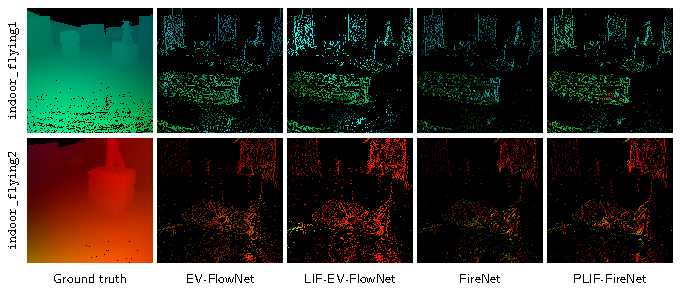
\includegraphics[width=0.95\textwidth]{04_chapters/NeurIPS21/figures/qualitative2.pdf}
	\caption{Qualitative evaluation of our best performing ANNs and SNNs on sequences from the MVSEC dataset \cite{zhu2018multivehicle}. The optical flow color-coding scheme can be found in \figref{fig:neurips_flowcode}.}
	\label{fig:neurips_qualitative}
\end{figure}

\subsection{Evaluation of the ANN and SNN architectures}\label{sec:neurips_annsnn}

Firstly, the quantitative results in \tabref{tab:neurips_flowevluation} confirm the validity of the proposed SSL framework for event-based optical flow estimation with recurrent networks. As shown, our base architectures EV-FlowNet and FireNet perform on par with the current state-of-the-art, even though these non-recurrent networks from literature encode explicit temporal information in their input event representations, and were trained on other very similar sequences from MVSEC \cite{zhu2018multivehicle} to prevent the input statistics from deviating from the training distribution during inference \cite{lee2020spikeflownet,zhu2018evflownet,zhu2019unsupervised}. Since we train on a very different dataset \cite{delmerico2019are}, this on-par performance also confirms the generalizability of our ANNs and SNNs to distinctly different scenes and distributions of optical flow vectors. This claim is further supported by qualitative results in \figref{fig:neurips_qualitative} and additional results in \secref{sec:neurips_appendix}.\newpage

Secondly, from the comparison between our base ANN architectures and their spiking counterparts without adaptation mechanisms (i.e., LIF-EV-FlowNet and LIF-FireNet), we can conclude that, although there is a general increase in the EPE and the percentage of outliers when going spiking, the proposed SNNs are still able to produce high quality event-based optical flow estimates. In fact, according to \tabref{tab:neurips_flowevluation}, the main drop in accuracy does not come from the incorporation of the spiking function (and the selection of $\text{aTan}'$ as surrogate gradient), but mainly from the use of vanilla convolutional recurrent layers instead of gated recurrent units. As shown, our spiking LIF architectures perform very close to their RNN and leaky counterparts, despite the latter being ANNs. This highlights the important need for more powerful convolutional recurrent units for SNNs, similar to ConvLSTMs \cite{shi2015convolutional} and ConvGRUs \cite{ballas2016delving} for ANNs, as this would narrow the performance gap between these two processing modalities according to our observations. Interestingly, a previous comparison of the performance of recurrent ANNs and SNNs for event-based classification \cite{he2020comparing} suggested similar improvements to SNN units.

\subsection{Impact of adaptive mechanisms for spiking neurons}\label{sec:neurips_adaptive}

Table \ref{tab:neurips_flowevluation} also allows us to draw conclusions about the effectiveness of the adaptive mechanisms for spiking neurons introduced in \secref{sec:neurips_neurons}. For both EV-FlowNet and FireNet, we observe that threshold adaptation based on postsynaptic activity (i.e., the ALIF model) performs worse compared to other models. While the ALIF model was shown to be effective for learning long temporal dependencies from relatively low-dimensional data as in \cite{bellec2018long,bellec2020solution,yin2021accurate}, the adaptation delay introduced by relying on a postsynaptic signal seems detrimental when working with fast-changing, high-dimensional event data. This is in line with suggestions by Paredes-Vall\'es \textit{et al.} in \cite{paredes-valles2020unsupervised}, who use presynaptic adaptation for this reason. Our own results with presynaptic adaptation (i.e., PLIF and XLIF models) are somewhat inconclusive. While PLIF performs better in the case of FireNet, this is not the case for EV-FlowNet. On the other hand, XLIF's performance is very similar to the LIF model for both FireNet and EV-FlowNet architectures. Based on these observations, we think that adaptivity based on presynaptic activity should be considered for further development. In this regard, the XLIF model has the advantage that it is able to generate activity (leading to gradient flow, and thus learning) even for very small inputs, whereas PLIF is incapable of this for a given threshold (because $P$ is always positive). A more detailed comparison of activity levels for the different variants is given in \secref{sec:neurips_appendix}, along with an approximation of the energy efficiency gains of SNNs compared to ANNs.

\subsection{Further lessons on training deep SNNs}\label{sec:neurips_lessons}

Multiple problems arise when training deep SNNs for a regression task that involves sparse data, as is done here. Regarding learning, we find that gradient vanishing poses the main issue. Even considering dense inputs/loss and a shallow (in timesteps or in layers) SNN, sufficient gradient flow is a result of wide enough (in our case, covering at least $\lvert U - \theta\rvert \leq \theta$) and properly scaled (i.e., $\leq 1$) surrogate gradients \cite{ledinauskas2020training,yin2021accurate,zenke2021remarkable}, and parameter initializations that lead to non-negligible amounts of spiking activity \cite{zenke2021remarkable}. Sparse data and deep networks make finding the proper settings more difficult, and for this reason, we have tried to increase the robustness of various of these hyperparameter settings.
First, we looked at the learning performance and gradient flow of networks with various surrogate gradient shapes and widths. Compared to the $\text{aTan}'$ surrogate specified in \secref{sec:neurips_neurons}, SuperSpike \cite{zenke2018superspike} with $\gamma = 10$ and $\gamma=100$ (both narrower) show little learning due to negligible gradient flow (see \secref{sec:neurips_appendix} for more details). One way of reducing the effect of a too narrow surrogate gradient would be to trigger spiking activity through regularization terms in the loss function, as done in, e.g., \cite{bellec2020solution,zenke2021remarkable}. These form a direct connection between loss and the neuron in question, bypassing most of the gradient vanishing that would happen in later layers. We tried the variant proposed in \cite{zenke2021remarkable}, which is aimed at achieving at least a certain fraction of neurons to be active at any given time. With this fraction set to $5\%$, we saw that for SuperSpike with $\gamma=10$ there was some learning happening, while for $\gamma=100$ there was no effect. Plots of the loss curves and gradient magnitudes are available in \secref{sec:neurips_appendix}. Of course, more research into these and other regularization methods is necessary. Alternatively, as done in \cite{ledinauskas2020training}, batch normalization (or other presynaptic normalization mechanisms) could be used to ensure proper activity and gradient flow.

Regarding the network output, there seems to be an intuitive gap between classification and regression tasks, with the latter requiring a higher resolution to be solved successfully. In our view, there are two aspects to this that might pose an issue to SNNs. First, given the single prediction layer that the here-presented SNNs have to go from binary to real-valued activations, one could expect a loss in output resolution compared to equivalent ANN architectures. Second, even for moderate activity levels, the outputs of a spiking layer can be much larger in magnitude than an equivalent ANN layer, even for comparable parameter initializations. Intuitive solutions to these shortcomings are (i) to increase the number of channels to increase the resolution, and (ii) to initialize the weights of the non-spiking prediction layer as to have a smaller magnitude. While increasing the number of output channels in $\mathcal{E}_5$ (LIF-FireNet, see \figref{fig:neurips_networks}) did not lead to significantly improved performance or learning speed, decreasing the initialization magnitude of the weights in layer $\mathcal{P}$ did. %As the loss curves in \appref{app:neurips_lessons} show, the improved initialization leads to faster convergence and less variability across neuron models and the selection of learnable parameters.

\begin{figure}[!b]
	\centering
	\captionsetup[subfigure]{justification=centering}
	\begin{subfigure}[b]{\textwidth}
		\includegraphics[width=1
		\textwidth]{04_chapters/NeurIPS21/figures/iwe.pdf}
		\caption{Sequence: poster\_6dof.}
	\end{subfigure}
	\begin{subfigure}[b]{\textwidth}
		\includegraphics[width=1
		\textwidth]{04_chapters/NeurIPS21/figures/iwe2.pdf}
		\caption{Sequence: shapes\_6dof.}
	\end{subfigure}
	\caption{Effect of scaling $\mathcal{L}_{\text{contrast}}$ for different optical flow vectors for two event partitions from the Event-Camera Dataset \cite{mueggler2017eventcamera}. Numbers on top indicate the maximum per-axis pixel displacement for each column.}
	\label{fig:neurips_loss}
\end{figure}

\newpage
\subsection{Additional experiments}\label{sec:neurips_appendix}

\subsubsection*{Convexity of the self-supervised loss function}\label{app:neurips_loss}

To evaluate the convexity of the self-supervised loss function for event-based optical flow estimation from \cite{zhu2019unsupervised} and the adaptation that we propose in this work, we conducted an experiment with two partitions of 40k events from the ECD dataset \cite{mueggler2017eventcamera}. In this experiment, for the selected partitions, we computed the value of \eqnref{eq:neurips_flow_loss} (with and without the scaling) for four sets of optical flow vectors given by:
\begin{align}
	\boldsymbol{u}_s(d) = \{(u:u=g(i, d), v:v&=g(j, d)), i\in\{0, 1, ..., 128\}, j\in\{0, 1, ..., 128\}\}\\
	g(x, d) &= \frac{2xd}{128}-d
\end{align}
where $d$ denotes the per-axis maximum displacement, which is drawn from the set $\smash{D=\{128, 256, 512, 1024\}}$. This is equivalent to performing a grid search for the lowest $\smash{\mathcal{L}_{\text{contrast}}}$ over an optical flow space ranging from $(-d, -d)$ to $(d, d)$ with 128 samples for each axis. \figref{fig:neurips_loss} highlights the main difference between the original and our adapted formulation. Although for the smaller values of $d$ the two normalized losses look qualitatively similar, for larger values it is possible to discern that the original $\mathcal{L}_{\text{contrast}}$ is not convex, and that its optimal solution is to throw events out of the image space during the warping process so they do not contribute to the computation of the loss. On the contrary, the scaling that we propose in \secref{sec:neurips_flow} fixes this issue, and results in a convex loss function for any value of $d$.

\subsubsection*{Self-supervised evaluation and additional qualitative results}\label{app:neurips_qual}

Apart from the quantitative and qualitative evaluation on the MVSEC dataset \cite{zhu2018multivehicle} included in \secref{sec:neurips_exp}, we also evaluate our architectures on the ECD \cite{mueggler2017eventcamera} and HQD \cite{stoffregen2020reducing} datasets, as in \cite{paredes-valles2021back,stoffregen2020reducing}. Since these datasets lack ground-truth data, we use the Flow Warp Loss (FWL$\uparrow$, higher is better) \cite{stoffregen2020reducing}, which measures the sharpness of the IWE relative to that of the original event partition using the variance as a measure of the contrast of the event images \cite{gallego2019focus}. In addition to FWL, we propose the Ratio of the Squared Average Timestamps (RSAT$\downarrow$, lower is better) as a novel, alternative metric to measure the quality of the optical flow without ground-truth data. Contrary to FWL, RSAT makes use of \eqnref{eq:neurips_scaling} to measure the contrast of the event images and is defined as:
\begin{equation}
	\text{RSAT} \doteq \frac{\mathcal{L}_{\text{contrast}}(t_{\text{ref}}^{\text{fw}}| \boldsymbol{u})}{\mathcal{L}_{\text{contrast}}(t_{\text{ref}}^{\text{fw}}|\boldsymbol{0})}
\end{equation}

\begin{wraptable}{r}{7cm}
	\vspace{5pt}
	\centering
	\resizebox{\linewidth}{!}{%
		{\renewcommand{\arraystretch}{1.1} 
			\begin{tabular}[b]{lccccc}
				\thickhline
				\thickhline
				& \multicolumn{2}{c}{ECD}&&\multicolumn{2}{c}{HQF}\\
				\cline{2-3}\cline{5-6}&FWL$\uparrow$&RSAT$\downarrow$&&FWL$\uparrow$&RSAT$\downarrow$ \\\thickhline
				EV-FlowNet & 1.31 & \textbf{0.94} && 1.37 & \textbf{0.92} \\
				RNN-EV-FlowNet & 1.36 & \underline{0.95} && 1.45 & \underline{0.93} \\
				Leaky-EV-FlowNet & 1.34 & \underline{0.95} && 1.39 & \underline{0.93} \\
				LIF-EV-FlowNet & 1.21 & \underline{0.95} && 1.24 & 0.94 \\
				ALIF-EV-FlowNet & 1.17 & 0.98 && 1.21 & 0.98 \\
				PLIF-EV-FlowNet & 1.24 & \underline{0.95} && 1.28 & \underline{0.93} \\
				XLIF-EV-FlowNet & 1.23 & \underline{0.95} && 1.25 & \underline{0.93} \\\hdashline
				FireNet & \textbf{1.43} & 0.99 && \textbf{1.57} & 0.99 \\
				RNN-FireNet & 1.34 & 0.99 && 1.42 & 0.99 \\
				Leaky-FireNet & \underline{1.40} & 0.99 && 1.52 & 0.99 \\
				LIF-FireNet & 1.28 & 0.99 && 1.34 & 1.00 \\
				ALIF-FireNet & 1.35 & 1.00 && \underline{1.49} & 1.00 \\
				PLIF-FireNet & 1.30 & 0.97 && 1.35 & 0.98 \\
				XLIF-FireNet & 1.29 & 0.99 && 1.39 & 0.99 \\
				\thickhline
				\thickhline
	\end{tabular}}}
	\captionof{table}{Quantitative evaluation on the ECD \cite{mueggler2017eventcamera} and HQF \cite{stoffregen2020reducing} datasets. Best in bold, runner up underlined.}
	\label{tab:neurips_flow}
\end{wraptable}

\noindent where $\text{RSAT}$$<$$1$ implies that the predicted optical flow is better than a baseline consisting of null vectors. Since both metrics are sensitive to the number of input events \cite{paredes-valles2020unsupervised}, we set $N$$=$$15$k events for all sequences in this evaluation. Quantitative results of this evaluation can be found in \tabref{tab:neurips_flow}, while qualitative results on these datasets are shown in \figref{fig:neurips_qualitative_add}.% The optical flow color-coding scheme is given in \figref{fig:neurips_colorcode}.

\begin{figure}[!t]
	\centering
	\includegraphics[width=\textwidth]{04_chapters/NeurIPS21/figures/qualitative_additional.pdf}
	\caption{Additional qualitative results of our best performing ANNs and SNNs on sequences from the ECD \cite{mueggler2017eventcamera} (top three) and HQF \cite{stoffregen2020reducing} (bottom three) datasets. The optical flow color-coding scheme can be found in \figref{fig:neurips_flowcode}.}
	\label{fig:neurips_qualitative_add}
\end{figure}

%\begin{figure}[!t]
%	\begin{minipage}{\textwidth}
%		\begin{minipage}[b]{0.275\textwidth}
%			\centering
%			\includegraphics[width=1
%			\textwidth]{04_chapters/NeurIPS21/figures/flow.png}
%			\captionof{figure}{Optical flow color-coding scheme. Direction is encoded in color hue, and speed in color brightness.}
%			\label{fig:neurips_colorcode}
%		\end{minipage}
%		\hfill
%		\begin{minipage}[b]{0.675\textwidth}
%			\centering
%			\resizebox{0.825\linewidth}{!}{%
%				{\renewcommand{\arraystretch}{1.1} 
%					\begin{tabular}[b]{lccccc}
%						\thickhline
%						\thickhline
%						& \multicolumn{2}{c}{ECD}&&\multicolumn{2}{c}{HQF}\\
%						\cline{2-3}\cline{5-6}&FWL&RSAT&&FWL&RSAT \\\thickhline
%						EV-FlowNet & 1.31 & 0.94 && 1.37 & 0.92 \\
%						RNN-EV-FlowNet & 1.36 & 0.95 && 1.45 & 0.93 \\
%						Leaky-EV-FlowNet & 1.34 & 0.95 && 1.39 & 0.93 \\
%						LIF-EV-FlowNet & 1.21 & 0.95 && 1.24 & 0.94 \\
%						ALIF-EV-FlowNet & 1.17 & 0.98 && 1.21 & 0.98 \\
%						PLIF-EV-FlowNet & 1.24 & 0.95 && 1.28 & 0.93 \\
%						XLIF-EV-FlowNet & 1.23 & 0.95 && 1.25 & 0.93 \\\hdashline
%						FireNet & 1.43 & 0.99 && 1.57 & 0.99 \\
%						RNN-FireNet & 1.34 & 0.99 && 1.42 & 0.99 \\
%						Leaky-FireNet & 1.40 & 0.99 && 1.52 & 0.99 \\
%						LIF-FireNet & 1.28 & 0.99 && 1.34 & 1.00 \\
%						ALIF-FireNet & 1.35 & 1.00 && 1.49 & 1.00 \\
%						PLIF-FireNet & 1.30 & 0.97 && 1.35 & 0.98 \\
%						XLIF-FireNet & 1.29 & 0.99 && 1.39 & 0.99 \\
%						\thickhline
%						\thickhline
%			\end{tabular}}}
%		\captionof{table}{Quantitative evaluation on the ECD \cite{mueggler2017event} and HQF \cite{stoffregen2020train} datasets. For each dataset, we report the mean FWL \cite{stoffregen2020train} (higher is better, $\uparrow$) and RSAT ($\downarrow$). Best in bold, runner up underlined.}
%		\label{tab:neurips_flow}
%		\end{minipage}
%	\end{minipage}
%\end{figure}

Apart from further confirming the generalizability of our architectures to other datasets and the on-par performance of our SNNs with respect to the recurrent ANNs (and thus to the state-of-the-art), results from this evaluation reveal the lack of robustness of the self-supervised FWL metric from Stoffregen and Scheerlinck \textit{et al.} \cite{stoffregen2020reducing} in capturing the quality of the learned event-based optical flow. As shown in \tabref{tab:neurips_flow}, FWL results do not correlate with the EPEs reported in \tabref{tab:neurips_flowevluation}. For instance, FireNet variants are characterized by higher values (thus better, according to \cite{stoffregen2020reducing}) than their computationally more powerful EV-FlowNet counterparts overall, while, according to \tabref{tab:neurips_flowevluation}, it should be the opposite. On the other hand, according to its correlation with the reported EPEs in \tabref{tab:neurips_flowevluation}, RSAT, which is based on our reformulation of the self-supervised loss function from \cite{zhu2019unsupervised}, is a more reliable metric to assess the quality of event-based optical flow without ground-truth data.

\begin{figure}[!t]
	\centering
	\includegraphics[trim=0 150 0 3, clip, width=0.85\textwidth]{04_chapters/NeurIPS21/figures/qualitative3.pdf}
	\caption{Qualitative results of FireNet and FireFlowNet variants on a sequence from MVSEC \cite{zhu2018multivehicle}. The optical flow color-coding scheme can be found in \figref{fig:neurips_flowcode}.}
	\label{fig:neurips_qualitative_recurrency}
\end{figure}

\subsubsection*{Ablation study on recurrent connections}\label{app:neurips_recurrency}

In this ablation study, we evaluate the importance of explicit recurrent connections for event-based optical flow estimation with ANNs and SNNs when using our input event representation (see \secref{sec:neurips_input}) and training settings (see \secref{sec:neurips_exp}). To do this, we use the base FireNet architecture and its leaky and LIF variants (as introduced \secref{sec:neurips_nets}), and compare their performance on MVSEC \cite{zhu2018multivehicle} to their non-recurrent counterparts. As in \cite{paredes-valles2021back}, the non-recurrent version of FireNet that we use, which substitutes the ConvGRUs with convolutional encoders, is further referred to as FireFlowNet. The qualitative and quantitative results for this ablation study are shown in \figref{fig:neurips_qualitative_recurrency} and \tabref{tab:neurips_flowablation}, respectively.

Firstly, from these results, we can conclude that stateless ANNs (such as FireFlowNet) are not capable of learning to estimate optical flow using our input event representation and training pipeline. This observation confirms the claim made in \secref{sec:neurips_input} about the fact that our event representation minimizes the amount of temporal information encoded in the input to the networks. Secondly, these results also confirm that, in order to successfully learn optical flow, the networks need to be able to build an internal (hidden) state through explicit recurrent connections and/or neural dynamics. As shown, the only architecture that is not able to learn optical flow is FireFlowNet. If this network is augmented with recurrent connections (i.e., FireNet), neural dynamics (i.e., Leaky-FireFlowNet, LIF-FireFlowNet), or both (i.e., Leaky-FireNet, LIF-FireNet), optical flow can be learned with our proposed pipeline and event representation. However, from the quantitative results in \tabref{tab:neurips_flowablation}, we can observe that learning optical flow through neural dynamics without explicit recurrent connections (i.e., Leaky-FireFlowNet, LIF-FireFlowNet), although possible, is quite complex and results in networks with lower accuracy. For this reason, we conclude that recurrent connections are an important driver for learning accurate event-based optical flow with our training pipeline, and hence, we use them in the ANNs and SNNs that we propose in this work.

%\begin{figure}[!b]
%	\centering
%	\includegraphics[width=0.65\textwidth]{04_chapters/NeurIPS21/figures/lcurves_recurr.pdf}
%	\caption{Training loss curves of FireNet and FireFlowNet variants.}
%	\label{fig:neurips_recurr}
%\end{figure}

%Additionally, we plotted the training loss curves for the various architectures in \figref{fig:neurips_recurr}. These do not paint the same picture as the quantitative evaluation results in \tabref{tab:neurips_flowablation}: for instance, the EPEs of Leaky-FireFlowNet are worse than those of FireNet, but their training losses suggest otherwise. This could be caused by different networks focusing on different parts of the loss: without recurrent connections, decreasing $\mathcal{L}_\text{contrast}$ may be more difficult, whereas focusing efforts on $\mathcal{L}_\text{smooth}$ might still allow for decreasing the overall loss $\mathcal{L}_\text{flow}$. While resulting in similar training losses, the latter approach does not lead (as much) to the actual learning of optical flow.

\begin{table*}[!t]
	\centering
	\resizebox{1\linewidth}{!}{%
		{\renewcommand{\arraystretch}{1.1} 
			\begin{tabular}{lccccccccccc}
				\thickhline
				\thickhline
				\multirow{2}{*}{${\text{dt}=1}$} & \multicolumn{2}{c}{outdoor\_day1}&& \multicolumn{2}{c}{indoor\_flying1} && \multicolumn{2}{c}{indoor\_flying2} && \multicolumn{2}{c}{indoor\_flying3}\\\cline{2-3}\cline{5-6}\cline{8-9}\cline{11-12}
				& EPE$\downarrow$ & $\%_{\text{Outlier}}$$\downarrow$&& EPE$\downarrow$ & $\%_{\text{Outlier}}$$\downarrow$&& EPE$\downarrow$ & $\%_{\text{Outlier}}$$\downarrow$&& EPE$\downarrow$ & $\%_{\text{Outlier}}$$\downarrow$\\\thickhline
				FireNet & \underline{0.55} & \textbf{0.35} && \textbf{0.89} & \textbf{1.93} && \textbf{1.62} & \textbf{14.65} && \textbf{1.35} & \textbf{10.64} \\
				Leaky-FireNet & \textbf{0.52} & 0.41 && \underline{0.90} & 2.66 && \underline{1.67} & \underline{16.09} && \underline{1.43} & 13.16\\
				LIF-FireNet & 0.57 & \underline{0.40} && 0.98 & \underline{2.48} && 1.77 & 16.40 && 1.50 & \underline{12.81} \\
				\hdashline
				FireFlowNet & 1.02 & 1.62 && 1.37 & 6.86 && 2.24 & 25.74 && 2.00 & 21.09 \\
				Leaky-FireFlowNet & 0.61 & 0.56 && 0.97 & 2.71 && 1.76 & 17.68 && 1.52 & 14.16 \\
				LIF-FireFlowNet & 0.84 & 1.15 && 1.22 & 5.55 && 2.06 & 22.25 && 1.80 & 18.13 \\
				\thickhline
				\multirow{2}{*}{${\text{dt}=4}$} & & && & && & && & \\
				& & && & && & && & \\\thickhline
				FireNet & \underline{2.04} & \underline{20.93} && \textbf{3.35} & \underline{42.50} && \textbf{5.71} & \underline{61.03} && \textbf{4.68} & \underline{53.42} \\
				Leaky-FireNet & \textbf{1.96} & \textbf{18.26} && \underline{3.42} & \textbf{42.03} && \underline{5.92} & \textbf{58.80} && \underline{4.98} & \textbf{52.57}\\
				LIF-FireNet & 2.12 & 21.00 && 3.72 & 48.27 && 6.27 & 64.16 && 5.23 & 58.43\\
				\hdashline
				FireFlowNet & 3.88 & 55.47 && 5.29 & 68.37 && 8.26 & 79.42 && 7.33 & 78.69 \\
				Leaky-FireFlowNet & 2.29 & 24.22 && 3.68 & 47.12 && 6.29 & 62.30 && 5.37 & 58.29 \\
				LIF-FireFlowNet & 3.24 & 43.08 && 4.67 & 60.34 && 7.54 & 74.68 && 6.54 & 71.45 \\
				\thickhline
				\thickhline
	\end{tabular}}}
\caption{Quantitative evaluation of FireNet and FireFlowNet variants on MVSEC \cite{zhu2018multivehicle}. Best in bold, runner up underlined.}
\label{tab:neurips_flowablation}
\end{table*}

\subsubsection*{Ablation study on learnable parameters for SNNs}\label{app:neurips_learnable}

Several works emphasize the importance of including neural parameters in the optimization \cite{fang2021incorporating,perez-nieves2021neural,yin2021accurate,zenke2021visualizing}, agreeing that including the various decays or leaks is beneficial for performance. Some also argue and show that learning thresholds adds little value \cite{fang2021incorporating,perez-nieves2021neural}, which makes intuitive sense given that the same effect can be achieved through scaling the synaptic weights. To confirm these observations, we perform an ablation study on the learning of per-channel leaks and thresholds for LIF-FireNet. All instances of a parameter are initialized to the same value, but can be adapted over time in the case of learning. 
%Initialization details can be found in \appref{app:neurips_init}. 
The results in \tabref{tab:neurips_ablation} suggest that, for our task, learning at least the leaks is beneficial for performance. However, despite these differences in EPE, the training loss curves for all variants, as shown in \figref{fig:neurips_ablation}, do not vary a lot. For this we can follow the same explanation as in the ablation study on recurrent connections: without the optimization of leaks, the network could focus on decreasing $\mathcal{L}_\text{smooth}$, which does not lead (as much) to the actual learning of optical flow.

Looking at the learned leaks also gives us insight into how information is integrated throughout the network. \figref{fig:neurips_leaks} shows the distribution of the parameter $a$, from which the membrane potential leaks are computed as $\smash{\alpha = \frac{1}{1 + \exp(-a)}}$, for the LIF-FireNet variants with learnable leaks. Initially, all $a = -4$; after learning, earlier layers mostly end up with faster leaks (lower $a$), while later layers end up with slower leaks (higher $a$). This intuitively makes sense: we want earlier layers to respond quickly to changing inputs, while we need later layers to (more slowly) integrate information over time and produce an optical flow estimate.

\begin{figure}[!t]
	\begin{minipage}{\textwidth}
		\begin{minipage}[t]{0.515\textwidth}
			\centering
			\includegraphics[width=1\textwidth]{04_chapters/NeurIPS21/figures/lcurves_ablation.pdf}
			\captionof{figure}{Training loss curves for LIF-FireNet variants with different sets of learnable parameters.}
			\label{fig:neurips_ablation}
		\end{minipage}
		\hfill
		\begin{minipage}[t]{0.45\textwidth}
			\centering
			\centering
			\vspace{-100pt}
			\resizebox{1\linewidth}{!}{%
				{\renewcommand{\arraystretch}{1.1} 
					\begin{tabular}{lcccc}
						\thickhline
						\thickhline
						Learnable thresholds & & X & & X\\
						Learnable leaks & & & X & X\\\thickhline
						outdoor\_day1 & 0.65 & 0.68 & \textbf{0.57} & \underline{0.58} \\
						indoor\_flying1 & 1.14 & 1.04 & \underline{0.97} & \textbf{0.96} \\
						indoor\_flying2 & 1.88 & 1.89 & \textbf{1.70} & \underline{1.82} \\
						indoor\_flying3 & 1.62 & 1.61 & \textbf{1.45} & \underline{1.52} \\
						\thickhline
						\thickhline
%						\vspace{50pt}
			\end{tabular}}}
		\captionof{table}{Ablation study on learnable parameters for SNNs on MVSEC \cite{zhu2018multivehicle} using variants of LIF-FireNet. We report the EPE$\downarrow$ for $\text{dt}=1$. Best in bold, runner up underlined.}
		\label{tab:neurips_ablation}
		\end{minipage}
	\end{minipage}
\end{figure}

\begin{figure}[!t]
	\captionsetup[subfigure]{justification=centering}
	\centering
	\begin{subfigure}[b]{0.49\textwidth}
		\centering
		\includegraphics[width=1\textwidth]{04_chapters/NeurIPS21/figures/ablation_leaks_onlyleak.pdf}
		\caption{Variant with learnable leaks.}
	\end{subfigure}
	\hfill
	\begin{subfigure}[b]{0.49\textwidth}
		\centering
		\includegraphics[width=1\textwidth]{04_chapters/NeurIPS21/figures/ablation_leaks_both.pdf}
		\caption{Variant with learnable leaks and thresholds.}
	\end{subfigure}
	\caption{LIF-FireNet distribution of learned leaks $\alpha = \frac{1}{1 + \exp(-a)}$, initialized at $a = -4$.}
	\label{fig:neurips_leaks}
\end{figure}

%\subsubsection*{Training loss curves of adaptive SNNs}\label{app:neurips_learning}
%
%To support the conclusions derived in \secref{sec:neurips_adaptive}, \figref{fig:neurips_adapt} presents the training loss curves for our EV-FlowNet and FireNet spiking architectures with the different adaptive mechanisms introduced in \secref{sec:neurips_neurons}. As shown, while the curves for presynaptic adaptation (i.e., the PLIF and XLIF neuron models) are very similar to that of the LIF model, the loss curve of the ALIF model suggests the unsuitableness of postsynaptic adaptation when working with event data for optical flow estimation.
%
%\begin{figure}[!h]
%	\centering
%	\begin{subfigure}[b]{0.49\textwidth}
%		\centering
%		\includegraphics[width=1\textwidth]{04_chapters/NeurIPS21/figures/lcurves_evflownet.pdf}
%		\caption{EV-FlowNet variants.}
%	\end{subfigure}
%	\hfill
%	\begin{subfigure}[b]{0.49\textwidth}
%		\centering
%		\includegraphics[width=1\textwidth]{04_chapters/NeurIPS21/figures/lcurves_adapt.pdf}
%		\caption{FireNet variants.}
%	\end{subfigure}
%	\caption{Training loss curves of our SNNs with different adaptive mechanisms.}
%	\label{fig:neurips_adapt}
%\end{figure}

%\subsubsection*{Hyperparameter and initialization details}\label{app:neurips_init}
%
%Weights and biases of ANN modules follow the default \texttt{Conv2d} PyTorch initialization $\smash{\mathcal{U}(-1/p, 1/p)}$, with $\smash{p = \sqrt{c_\text{in} \cdot k_1 \cdot k_2}}$, $c_\text{in}$ the number of input channels and $\smash{\{k_1, k_2\}}$ the kernel sizes. For the SNN modules, we take $\smash{p = \sqrt{c_\text{in}}}$ for the weights to ensure enough activity, and include no biases. In the case of SNNs, we also changed the weight initialization of the prediction layer $\mathcal{P}$ to $\smash{\mathcal{U}(-0.01, 0.01)}$ in order to improve learning stability, as explained in \appref{app:neurips_lessons}. The $\text{aTan}'$ surrogate gradient has width $\gamma=10$; also see \appref{app:neurips_lessons} for a visualization.
%
%\tabref{tab:neurips_init} gives the leak and threshold parameters of the SNNs for the performed experiments. Membrane leak $\alpha$, threshold leak $\eta$, and trace addition/leak $\rho_{\{0, 1\}}$ are clamped through a sigmoid function, e.g., $\smash{\alpha = \frac{1}{1 + \exp(-a)}}$, to prevent instability \cite{fangIncorporatingLearnableMembrane2021}. For $\alpha$, $\eta$ and $\rho_{\{0,1\}}$ the (learnable) parameters in the sigmoid function are $a$, $n$ and $p_{\{0,1\}}$, respectively. Threshold $\theta$ and the parameters of the adaptive threshold $\beta_{\{0, 1\}}$ are clamped to $[0.01, \rightarrow)$, $[0.01, \rightarrow)$ and $[0, \rightarrow)$, respectively.
%
%\begin{table}[!h]
%	\centering
%	\caption{SNN parameter initializations.}
%	\vspace{7pt}
%	\label{tab:neurips_init}
%	{\renewcommand{\arraystretch}{1.3} 
%		\begin{tabular}{lcc}
%			\thickhline
%			\thickhline
%			& \multicolumn{2}{c}{Section / Appendix}                         \\ \cline{2-3}
%			& \multicolumn{1}{c}{\ref{sec:neurips_annsnn}-\ref{sec:neurips_lessons}, \ref{app:neurips_qual}, \ref{app:neurips_recurrency} and \ref{app:neurips_lessons}} & \multicolumn{1}{c}{\ref{app:neurips_learnable}} \\
%			\thickhline
%			$a$       & $\mathcal{N}(-4, 0.1)$               & $-4$                  \\
%			$n$       & $\mathcal{N}(-2, 0.1)$               & -                      \\
%			$p_0$     & $\mathcal{N}(-2, 0.1)$               & -                    \\
%			$p_1$     & $\mathcal{N}(-2, 0.1)$               & -                       \\
%			$\theta$  & $\mathcal{N}(0.8, 0.1)$              & $0.8$                 \\
%			$\beta_0$ & $\mathcal{N}(0.3, 0.1)$              & -                      \\
%			$\beta_1$ & $\mathcal{N}(1, 0.1)$                & -                     \\
%			\thickhline
%			\thickhline
%	\end{tabular}}
%\end{table}

\subsubsection*{Details on further lessons}\label{app:neurips_lessons}

We looked at the effect of surrogate gradient width on learning performance by trying out three variants on LIF-FireNet: $\text{aTan}'$ with $\gamma=10$ (default), and SuperSpike \cite{zenke2018superspike} with $\gamma \in \{10, 100\}$. %; see \figref{fig:neurips_surrogate} for a comparison of their shapes. 
The resulting loss curves are plotted in \figref{fig:neurips_loss_actregul}. The width of $\text{aTan}'$-10 is such that there is sufficient gradient flow for learning; this is less so for SuperSpike-10, and not at all for SuperSpike-100. The plots of per-layer mean gradient magnitude in \figref{fig:neurips_grad_actregul} confirm this: SuperSpike-10 only shows non-negligible gradient flow for the last two layers, while the mean gradients for SuperSpike-100 are practically zero.

%\begin{figure}[!h]
%	\centering
%	\begin{subfigure}[b]{0.59\textwidth}
%		\centering
%		\includegraphics[width=\textwidth]{04_chapters/NeurIPS21/figures/lcurves_actregul.pdf}
%		\caption{Training loss curves belonging to LIF-FireNet.}
%		\label{fig:neurips_loss_actregul}
%	\end{subfigure}
%	\hfill
%	\begin{subfigure}[b]{0.39\textwidth}
%		\centering
%		\includegraphics[width=\textwidth]{04_chapters/NeurIPS21/figures/surrogates.pdf}
%		\caption{Surrogate gradients.}
%		\label{fig:neurips_surrogate}
%	\end{subfigure}
%	\caption{Impact of the choice of surrogate gradient $\sigma'$ and activity regularization $\mathcal{L}_\text{act}$. $\text{aTan}'$-10 denotes $\smash{\sigma'(x) = 1/(1 + 10x^2)}$, where $x = U - \theta$; SuperSpike-$\gamma$ \cite{zenkeSuperSpikeSupervisedLearning2018} denotes $\smash{\sigma'(x) = 1/(1 + \gamma \lvert x\rvert)^2}$, with $\gamma \in \{10, 100\}$.}
%\end{figure}

%\begin{figure}[!t]
%	\centering
%	\includegraphics[width=0.6\textwidth]{04_chapters/NeurIPS21/figures/lcurves_winit.pdf}
%	\caption{Mean and inter-quartile range (shaded area) of training loss curves belonging to LIF-FireNet variants with the PyTorch default weight initialization based on incoming channels and kernel size, or our initialization $\mathcal{U}(-0.01, 0.01)$, which gives much smaller weights.}
%	\label{fig:neurips_winit}
%\end{figure}

As mentioned in \secref{sec:neurips_lessons}, one possible way of mitigating gradient vanishing would be to connect each layer to the loss directly, through, e.g., a regularization term on minimum activity as in \cite{zenke2021remarkable}:
\begin{equation}
	\label{eq:neurips_actloss}
	\mathcal{L}_\text{act} = \sum_l^L \max(0, f_\text{desired} - f_\text{actual})^2
\end{equation}

\begin{figure}[!t]
	\centering
	\includegraphics[width=0.95\textwidth]{04_chapters/NeurIPS21/figures/gradients.pdf}
	\caption{Per-layer mean of absolute gradient values during training of LIF-FireNet with various surrogate gradients, and activity regularization $\mathcal{L}_\text{act}$. $\text{aTan}'$-10 denotes $\smash{\sigma'(x) = 1/(1 + 10x^2)}$, where $x = U - \theta$; SuperSpike-$\gamma$ \cite{zenke2018superspike} denotes $\smash{\sigma'(x) = 1/(1 + \gamma \lvert x\rvert)^2}$, with $\gamma \in \{10, 100\}$. Data is smoothed with a 1000-step moving average and a stride of 100.}
	\label{fig:neurips_grad_actregul}
\end{figure}

\begin{figure}[!t]
	\centering
	\includegraphics[width=0.65\linewidth]{04_chapters/NeurIPS21/figures/lcurves_actregul.pdf}
	\caption{Impact of the choice of surrogate gradient $\sigma'$ and activity regularization $\mathcal{L}_\text{act}$. $\text{aTan}'$-10 denotes $\smash{\sigma'(x) = 1/(1 + 10x^2)}$, where $x = U - \theta$; SuperSpike-$\gamma$ \cite{zenke2018superspike} denotes $\smash{\sigma'(x) = 1/(1 + \gamma \lvert x\rvert)^2}$, with $\gamma \in \{10, 100\}$. Training loss curves belonging to LIF-FireNet.}
	\label{fig:neurips_loss_actregul}
\end{figure}

\noindent with $L$ being all the spiking layers, $f_\text{desired}$ the desired per-timestep fraction of active neurons, and $f_\text{actual}$ the actual per-timestep fraction of active neurons. By taking the maximum, we ensure that $\mathcal{L}_\text{act}$ goes to zero as soon as the activity is above the desired level. The effect of adding activity regularization with $f_\text{desired} = 0.05$ can be observed in \figref{fig:neurips_loss_actregul}. While the direct connection between each layer and the loss is able to start learning for SuperSpike-10, it has little effect for SuperSpike-100. The bottom row of \figref{fig:neurips_grad_actregul} shows that the gradient flow for SuperSpike-10 becomes non-negligible for earlier layers after step 40,000 or so; for SuperSpike-100, the gradients have increased significantly, but are still not enough to allow learning. 
These results are in line with the recent SNN literature, which shows that SuperSpike-100 can enable learning for shallow networks \cite{perez-nieves2021neural,zenke2021remarkable}, but that it degrades performance as the number of layers increases beyond four \cite{ledinauskas2020training}, and that tuning of the surrogate width is necessary. Note that \cite{ledinauskas2020training} also demonstrates learning with SuperSpike-10 for deeper networks, but this probably works because they use batch normalization.

%Additionally, we tried different weight initializations for the prediction layer $\mathcal{P}$, based on the observation that SNNs may need smaller weights than comparable ANNs to get to similar outputs. We performed training runs with the \{LIF, ALIF, PLIF, XLIF\}-FireNet variants (see \tabref{tab:neurips_flowevluation}) and the LIF-FireNet parameter ablations (\appref{app:neurips_learnable}) with (i) $\smash{\mathcal{U}(-1/\sqrt{32}, 1/\sqrt{32})}$ (default PyTorch initialization), and (ii) $\smash{\mathcal{U}(-0.01, 0.01)}$, which gives weights approximately 18x smaller. \figref{fig:neurips_winit} shows the inter-quartile range (IQR) and mean for both variants.
%
%Clearly, $\smash{\mathcal{U}(-0.01, 0.01)}$ improves convergence speed and decreases variability. In fact, ALIF-FireNet with $\smash{\mathcal{U}(-1/\sqrt{32}, 1/\sqrt{32})}$ failed to converge at all, hence the mean deviating from the IQR. This was not a problem with the smaller weight initialization.

\begin{figure}[!t]
	\centering
	\begin{subfigure}[t]{0.48\textwidth}
		\centering
		\includegraphics[width=0.96\textwidth]{04_chapters/NeurIPS21/figures/activity_aee.pdf}
		\caption{EPE against mean activity (over all spiking layers).}
		\label{fig:neurips_act_EPE}
	\end{subfigure}
	\hfill
	\begin{subfigure}[t]{0.48\textwidth}
		\centering
		\includegraphics[width=\textwidth]{04_chapters/NeurIPS21/figures/activity_flow.pdf}
		\caption{Mean (normalized) optical flow magnitude (over all pixels that have at least one event) against mean activity (over all spiking layers). 
			%		The activity of the input $\boldsymbol{\varepsilon}^{\text{inp}}_k$ is identical for all networks, but is here plotted against the LIF-FireNet output.
		}
		\label{fig:neurips_act_flow}
	\end{subfigure}
	\caption{Recorded activity (fraction of nonzero values) of spiking FireNet variants during (a) indoor\_flying1 of MVSEC \cite{zhu2018multivehicle} with $\text{dt} = 1$ and (b) boxes\_6dof of the ECD dataset \cite{mueggler2017eventcamera} with $N=15$k events. Each marker represents one timestep.}
	\label{fig:neurips_allact}
\end{figure}

\subsubsection*{Comparison of activity levels for adaptive SNNs}\label{app:neurips_activity}

SNNs implemented in neuromorphic hardware consume less energy as their activity decreases \cite{davies2021advancing}, which makes it important to investigate how activity levels vary across spiking neuron models, and how they correlate with the outputs of the network: because spiking layers emit only binary spikes, in some cases more spikes would be needed for output values larger in magnitude. We recorded the activity (fraction of nonzero values) and EPE of the \{LIF, ALIF, PLIF, XLIF\}-FireNet variants during the indoor\_flying1 sequence of MVSEC \cite{zhu2018multivehicle} with $\text{dt} = 1$, as well as the mean normalized output optical flow magnitude during the boxes\_6dof sequence of the ECD dataset \cite{mueggler2017eventcamera} with $N=15$k input events. \figref{fig:neurips_allact} shows the results. One observation we can make from \figref{fig:neurips_act_EPE} is that the neuron models with an adaptive threshold (ALIF, XLIF) are more active than those without, while achieving similar EPEs. While this excessive spiking could be the result of initializing the base threshold $\beta_0$ too low, the similarity in EPE certainly suggests that these models spike too much for the performance they achieve, and that there is a certain redundancy in their activity.

Looking at \figref{fig:neurips_act_flow}, we again observe that the models with adaptive threshold are more active than those without. On the other hand, it seems that ALIF and XLIF are more consistent in their activity across the range of outputs (narrower, more vertically oriented clusters). Looking at the clusters of LIF and PLIF, we can see that they both have roughly the same shape, but the latter's average output is larger in magnitude. This indicates that presynaptic and postsynaptic adaptive mechanisms can both serve a purpose: the former helps in increasing the absolute output range, while the latter helps in keeping activity (and therefore energy consumption) constant across this range. This makes the XLIF model especially interesting to investigate further in future work.

To approximate the efficiency gains of SNNs running on neuromorphic hardware and compare it with equivalent ANN implementations, we can look at the number of accumulate (AC) and multiply-and-accumulate (MAC) operations of each, as is also done in \cite{yin2021accurate}. Using energy numbers for ACs and MACs from \cite{horowitz201411}, this gives us a very rough 25x increase in energy efficiency of SNNs compared to ANNs, assuming that (i) floating-point MAC operations cost five times as much energy as floating point AC operations; (ii) SNNs only make use of AC operations, while ANNs only make use of MAC operations; (iii) the average activity level of the SNN is 20\%, as in \figref{fig:neurips_act_EPE}. However, as rightly pointed out in \cite{davies2021advancing} (which contains a more elaborate quantification of efficiency gains of SNNs running on the Loihi neuromorphic processor), the comparison using AC and MAC operations for respectively SNNs and ANNs may not be a fair one for all tasks, considering, e.g., overhead in neuromorphic chips and the optimization of MACs in ANN accelerators.

\section{Conclusion}

In this chapter, we presented the first set of deep SNNs to successfully solve the real-world, large-scale problem of event-based optical flow estimation. To achieve this, we first reformulated the state-of-the-art training pipeline for ANNs to considerably shorten the time windows presented to the networks, approximating the way in which SNNs would receive spikes directly from the event camera. Additionally, we reformulated the state-of-the-art self-supervised loss function to improve its convexity. Prior to their training with this framework, we augmented several ANN architectures from literature with explicit and/or implicit recurrency, besides the addition of the spiking behavior. Extensive quantitative and qualitative evaluations were conducted on multiple datasets. Results confirm not only the validity of our training pipeline, but also the on-par performance of the proposed set of recurrent ANNs and SNNs with the self-supervised state-of-the-art. To the best of our knowledge, and especially due to the addition of explicit recurrent connections, the proposed SNNs correspond to the most complex spiking networks in the computer vision literature, architecturally speaking. For the SNNs, we also conducted several additional studies and (i) concluded that parameter initialization and the width of the surrogate gradient have a significant impact on learning: smaller weights in the prediction layer speed up convergence, while a too narrow surrogate gradient prevents learning altogether; and (ii) observed that adaptive mechanisms based on presynaptic activity outperform those based on postsynaptic activity, and perform similarly or better than the baseline without adaptation. Overall, we believe this chapter sets the groundwork for future research on neuromorphic processing for not only the event-based structure-from-motion problem, but also for other, similarly complex computer vision applications. For example, our results suggest the need for more powerful recurrent units for SNNs. %On another note, future work should also focus on the implementation of these deep SNNs on neuromorphic hardware, as it is there where these architectures excel due to the power efficiency that their sparse and asynchronous nature brings.

\section*{Supplementary material}
\vspace{10pt}
%\begin{itemize}
%	\setlength\itemsep{0.5em}
%	\item Video summary: \url{https://youtu.be/T7-9GGYnuZ4}
%	\item Project code: \url{https://github.com/tudelft/event_flow}
%\end{itemize}

\newlist{mylist_neurips}{itemize}{1}
\setlist[mylist_neurips]{label=\hspace{0pt}}
% \newcommand\itemoneneurips{\item \qrcode[height=0.4in]{https://youtu.be/T7-9GGYnuZ4}}
% \newcommand\itemtwoneurips{\item \qrcode[height=0.4in]{https://github.com/tudelft/event_flow}}
\newcommand\itemtwoneurips{\item \qrcode[height=0.4in]{https://mavlab.tudelft.nl/event_flow}}

\begin{mylist_neurips}[leftmargin=*, align=left, leftmargin=2em, itemindent=0pt, labelsep=0pt, labelwidth=2em]
	% \itemoneneurips\quad Video summary of the approach: \url{https://youtu.be/T7-9GGYnuZ4}
	\itemtwoneurips\quad Project page: \url{https://mavlab.tudelft.nl/event_flow}
\end{mylist_neurips}
	\chapter{Fully Neuromorphic Vision and Control for Autonomous Drone Flight}
\label{cha:sr}

{\it
Fede still had this at the non-final version, so there are quite some changes.
}

\blfootnote{The contents of this chapter have been published in:\\
	\vspace{-10pt}\begin{blockquote}
	F.\ Paredes-Vall\'es$^\dagger$, \textbf{J.\ J.\ Hagenaars}$^\dagger$, J.\ D.\ Dupeyroux$^\dagger$, S.\ Stroobants, Y.\ Xu, G.\ C.\ H.\ E.\ de Croon, \emph{Fully neuromorphic vision and control for autonomous drone flight}, Science Robotics, 2023.
\end{blockquote}%\vspace{-10pt}
Although not covered in this dissertation, this chapter also builds on the following publications:\\
\vspace{-10pt}\begin{blockquote}
	J.\ D.\ Dupeyroux, \textbf{J.\ J.\ Hagenaars}, F.\ Paredes-Vall\'es, G.\ C.\ H.\ E.\ de Croon, \emph{Neuromorphic control for optic-flow-based landing of MAVs using the Loihi processor}, IEEE International Conference on Robotics and Automation (ICRA), 2021.\\
	\textbf{J.\ J.\ Hagenaars}, F.\ Paredes-Vall\'es, G.\ C.\ H.\ E.\ de Croon, \emph{Evolved neuromorphic control for high speed divergence-based landings of MAVs}, IEEE Robotics and Automation Letters (RA-L), 2020.
\end{blockquote}%\vspace{-10pt}
{\scriptsize$\dagger$~~Equal contribution.}\\
$\text{}$\\
\textbf{Contribution:} The research in this chapter was a collaborative effort with multiple researchers, all from the Micro Air Vehicle Laboratory (Delft University of Technology). We all contributed equally to the conception of the study, to performing the experiments, and to the analysis of the results. My main contribution lay in the design and implementation of the control pipeline. This involved training neural control in simulation, designing the interface with the vision-based state estimation, and ensuring a successful sim-to-real transfer.
}

\newpage
\thispagestyle{empty}
\phantom{blabla}
\newpage

\section{Introduction}

\dropcap{O}ver the past decade, deep artificial neural networks (ANNs) have revolutionized the field of artificial intelligence. Among the successes has been the substantial improvement of visual processing, to an extent that computer vision can now outperform humans on specific tasks \cite{ciresan2011committee}. Also the field of robotics has benefited from this development, with deep ANNs achieving state-of-the-art accuracy in tasks such as stereo vision \cite{cheng2020hierarchicala,gu2020cascadea}, optical flow estimation \cite{ilg2017flowneta,sun2018pwcnet,teed2020rafta}, segmentation \cite{yuan2021segmentation,liu2022swina}, object detection \cite{girshick2015fasta,redmon2018yolov3a,xu2021endtoend}, and monocular depth estimation \cite{garg2016unsuperviseda,godard2017unsuperviseda,yuan2022newa}.
However, this high accuracy typically relies on substantial neural network sizes that require quite heavy and power-hungry processing hardware (tens of watts, hundreds of grams~\cite{nvidia}). This limits the number of tasks that can be performed by larger (ground) robots, and even prevents deployment on smaller robots with highly stringent resource constraints, like small flying drones. 

Neuromorphic hardware may provide a solution to this problem, since it mimics the energy-efficient, sparse and asynchronous nature of sensing and processing in biological brains~\cite{indiveri2000neuromorphica,sandamirskaya2022neuromorphic}. For example, the pixels in neuromorphic, event-based cameras only transmit information on brightness changes \cite{gallego2020eventbased}. Since typically only a fraction of the pixels change in brightness substantially, this leads to sparse vision inputs with subsequent events that are in the order of a microsecond apart. The asynchronous and sparse nature of visual inputs from event-based cameras represents a paradigm shift compared to traditional, frame-based computer vision. Ideally, processing would exploit these properties for quicker, more energy-efficient processing. However, currently, learning-based approaches to event-based vision involve accumulating events over a substantial amount of time, creating an ``event window'' that represents extended temporal information. This window is then processed similarly to a traditional image frame with an ANN \cite{zhu2018evflownet,zhu2019unsuperviseda,gehrig2021eraft,paredes-valles2021back}.
Although there is work that employs much shorter event windows \cite{paredes-valles2020unsupervised,hagenaars2021selfsupervised, paredes2023taming}, latency could be further reduced by processing events asynchronously as they come in. This could be performed by neuromorphic processors designed for implementing spiking neural networks (SNNs) \cite{maass1997networksa,gruning2014spikinga}. These networks have temporal dynamics more similar to biological neurons. In particular, the neurons have a membrane voltage that integrates incoming inputs and causes a spike when it exceeds a threshold. The binary nature of spikes allows for more energy-efficient processing than the floating point arithmetic in traditional ANNs \cite{davies2021advancing,ottati2023spikea}. The energy gain is further improved by reducing the spiking activity as much as possible, as is also a main property of biological brains \cite{sterling2015principlesa}. Coupling neuromorphic vision to neuromorphic processing promises low-energy and low-latency visual sensing and acting, as exhibited by agile animals such as flying insects \cite{muijres2014fliesa}.

However, in order to achieve these properties, several challenges have to be overcome related to present-day neuromorphic sensing and processing. For example, training is currently still much more difficult for SNNs than for ANNs \cite{pfeiffer2018deepa,tavanaei2019deepa}, mostly due to their sparse, binary, and asynchronous nature. The most well-known difficulty of SNN learning is the non-differentiability of the spiking activation function, which prevents naive application of backpropagation. Currently, this is tackled rather successfully with the help of surrogate gradients \cite{neftci2019surrogatea,zenke2021remarkable}, although longer sequences (as would be the case for event-by-event processing) can still lead to gradient vanishing. Moreover, although the richer neural dynamics can potentially represent more complex temporal functions, they are also harder to shape; and neural activity may saturate or dwindle during training, preventing further learning. The causes for this are hard to analyze, as there are many parameters that can play a role. Depending on the model, the relevant parameters may range from neural leaks and thresholds to recurrent weights and time constants for synaptic traces. A solution may lie in learning these parameters \cite{chowdhury2021understanding,fang2021incorporating}, but this further increases the dimensionality of the learning problem. Finally, when targeting a robotics application, SNN training and deployment is further complicated by the restrictions of existing embedded neuromorphic processing platforms. These restrictions were recently highlighted in a study on neuromorphic route learning \cite{zhu2023neuromorphic}, and include hardware and software challenges such as interfacing with neuromorphic cameras, the limitations of available neural models and\textemdash importantly\textemdash the still rather limited numbers of available neurons and synapses. To illustrate this latter point, the ROLLS chip~\cite{qiao2015reconfigurable} accommodates 256 spiking neurons, the Intel Kapoho Bay (featuring two Loihi chips \cite{davies2018loihi} in a USB stick form factor) features 262,100 neurons \cite{vitale2021eventdriven}, and the SpiNNaker version in \cite{galluppi2014eventbased} has 768,000 neurons. Although these chips differ in many more aspects than only the  number of neurons, this small sample already shows that current state-of-the-art SNNs cannot be easily embedded on robots. SNNs that have recently been trained on visually complex tasks such as optical flow determination \cite{paredes-valles2020unsupervised,hagenaars2021selfsupervised} still feature far too large network sizes for implementation on current neuromorphic processing hardware for embedded systems. The smallest size SNN in these studies is LIF-FireFlowNet (Leaky-Integrate and Fire) for optical flow estimation \cite{hagenaars2021selfsupervised}, which still has 3.7 million neurons (at an input resolution of 128$\times$128 pixels).

As a consequence, pioneering work in this area has been limited in complexity. Very early work involved the evolution of spiking neural network connectivity to map the 16 visual brightness inputs of a wheeled Kephera robot to its two motor outputs \cite{floreano2001evolution}. The evolved SNN, simulated in software, allowed the robot to avoid the walls in a black-and-white-striped environment. Most work exploring SNNs for robotic vision focuses on simulation. For example, in \cite{bing2018enda}, the events from a simulated event-based camera with 128$\times$128 pixels are accumulated into frames, compressing them over time into 8$\times$4 Poisson input neurons. These inputs, which capture the clear white lines of the road border, are then directly mapped to two output neurons for staying in the center of the road with the help of reward-modulated spike-time-dependent plasticity  learning. Robotic examples of in-hardware neuromorphic processing for vision are more rare. An early example is the one in \cite{galluppi2014eventbased}, in which an event-based camera with 128$\times$128 pixels is connected to a SpiNNaker neuromorphic processor to allow a driving robot to differentiate between two lights flashing at different frequencies with a 128-neuron winner-takes-all network. In \cite{milde2017obstacle} a spiking neural network is designed for following a light target in the top half of the field of view, while avoiding regions with many events in the bottom half of the field of view. This network is successfully implemented in the ROLLS neuromorphic chip~\cite{qiao2015reconfigurable} and tested in an office environment. Recent years have seen an increasing focus on flying robots (drones), because they need to react quickly while being extremely restricted in terms of size, weight, and power (SWaP). In \cite{vitale2021eventdriven}, an SNN is implemented on a bench-fixed dual-rotor to align the roll angle with a black-and-white disk located in front of the camera. The SNN involved both a visual Hough transform \cite{ballard1981generalizinga} for finding the line, and a proportional-derivative (PD) controller for generating the propeller commands. Finally, in \cite{dupeyroux2021neuromorphica}, an SNN was first evolved in simulation and then implemented in Loihi for vision-based landing of a flying drone. This control network only consisted of 35 neurons since the visual processing was still performed with conventional, frame-based computer vision methods. Additionally, it is worth noting that only the vertical motion of the drone was controlled with the SNN; its lateral position was controlled using traditional control algorithms and an external motion capture system. The current work represents a step up in complexity by performing three-dimensional visual ego-motion estimation and control of a flying drone with a fully neuromorphic vision-to-control pipeline.

In this chapter, we present a fully neuromorphic vision-to-control pipeline for controlling a flying drone, demonstrating the potential of neuromorphic hardware. The presented pipeline consists of a spiking neural network that is trained to accept raw event-camera data and output low-level control actions for performing autonomous vision-based ego-motion estimation and control at approximately 200 Hz. A core property of our learning setup is that it splits vision and control, which provides two major advantages. First, it helps to prevent the reality gap on the camera event input side, as the vision part is trained based on the raw events from the actual event camera on the drone. We use self-supervised learning, since this foregoes the need for ground truth measurements that are difficult to obtain for event-based vision. Second, as the output of the vision part is an ego-motion estimate, we can learn the control in a simple and extremely fast simulator. This allows us to evade the high-frequency generation of visually realistic images for event generation \cite{rebecq2018esim}, something that would lead to excessive training times in an end-to-end learning setup. 

\begin{figure*}[!t]
	\centering
	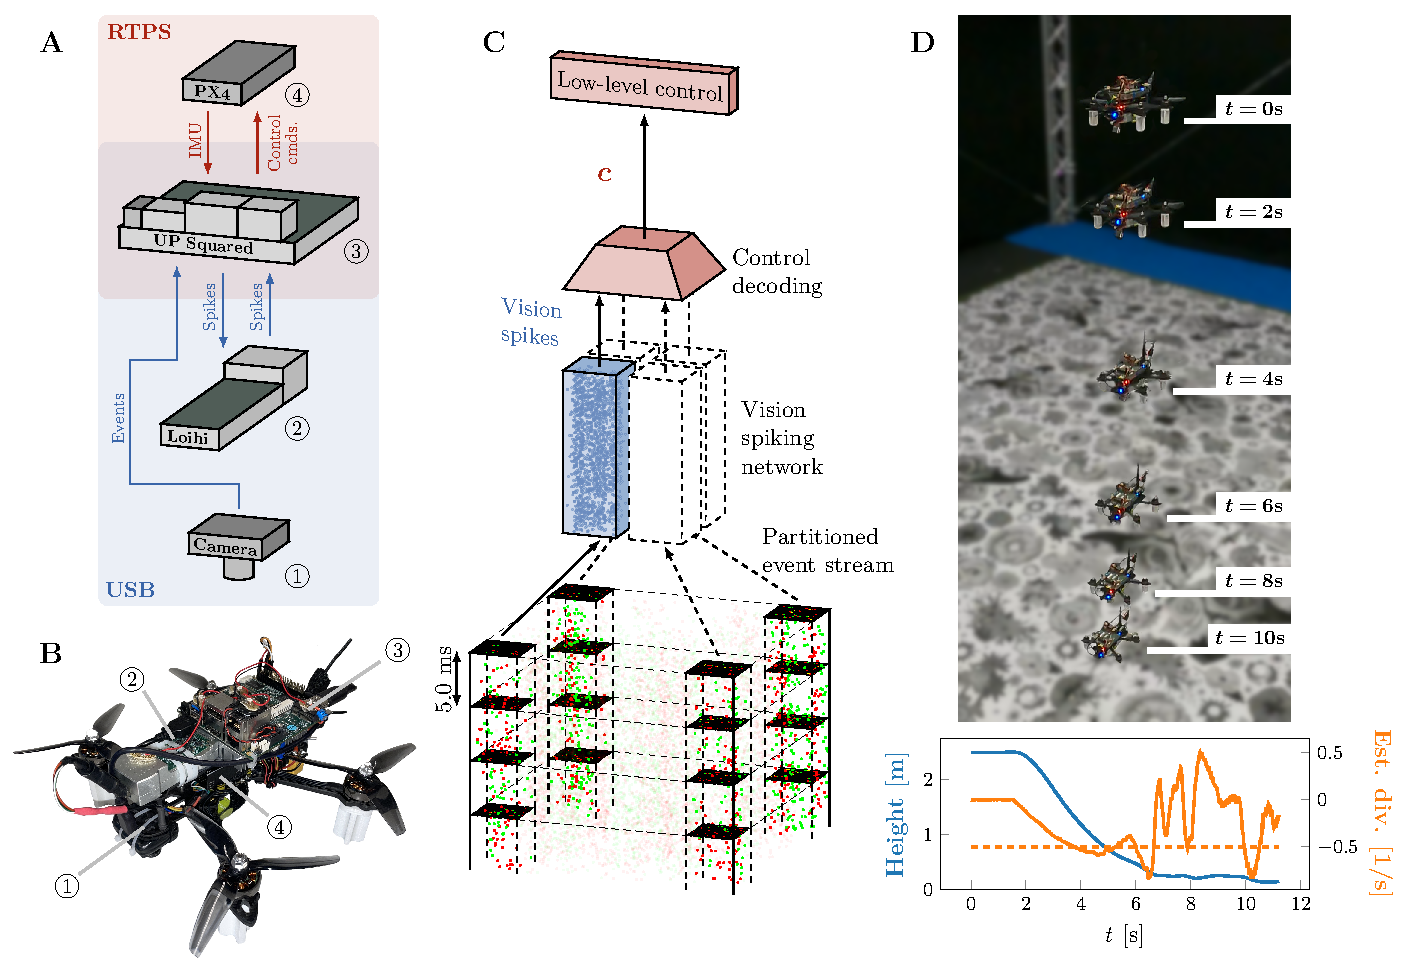
\includegraphics[width=\textwidth]{04_chapters/SR23/figures/fig1-pipeline.pdf}
	\caption{Overview of the proposed system. (\textit{A}) Hardware overview showing the communication between event-camera, neuromorphic processor, single-board computer and flight controller. RTPS (real-time publish-subscribe) and USB refer to the used communication protocols. (\textit{B}) Quadrotor used in this work (total weight 994 g, tip-to-tip diameter 35 cm). (\textit{C}) Pipeline overview showing events as input, processing by the vision network and decoding into a control command. (\textit{D}) Demonstration of the system for an optical flow constant divergence landing.} \label{fig:sr_pipeline}
\end{figure*}

\subsection*{A fully neuromorphic solution to vision-based navigation}

The fully neuromorphic vision-to-control pipeline, illustrated in \figref{fig:sr_pipeline}C, was implemented on the Loihi neuromorphic processor~\cite{davies2018loihi} and used on board a small flying robot (see \figref{fig:sr_pipeline}B) for vision-based navigation. A schematic of the hardware setup employed is shown in \figref{fig:sr_pipeline}A. The system successfully followed ego-motion setpoints (target values) in a fully autonomous fashion, without any external aids such as a positioning system. \figref{fig:sr_pipeline}D shows an example of a landing experiment with our neuromorphic pipeline in the control loop of the drone.
The figure shows the smoothly decreasing height of the drone above the ground (blue line), and the estimated optical flow divergence (orange line), which is the vertical component of the velocity vector divided by this height. The divergence curve is typical of an optical flow divergence landing, first approaching the setpoint -0.5~1/s and then becoming more oscillatory when getting very close to the ground~\cite{decroon2016monocular}.

As mentioned, the main challenge of deploying such a pipeline on embedded neuromorphic hardware is that, due to the preliminary state of this technology, one has to work within very tight limits regarding the available computational resources. In this project, several design decisions were made to adapt to these limitations. Firstly, the vision processing pipeline assumes that the event-based camera on the drone, the DVS 240~\cite{brandli2014240a}, looks down at a static, texture-rich, flat surface. Knowing the structure of the visual scene in advance simplifies the estimation of the ego-motion of the camera (and hence of the drone) with the help of optical flow information, as in \cite{decroon2013opticflow,decroon2016monocular,pijnackerhordijk2018vertical,hagenaars2020evolveda,dupeyroux2021neuromorphica}. Optical flow, or the apparent motion of scene points in the image space, can be estimated from the output of an event-based camera with a wide variety of methods, ranging from sparse feature-tracking algorithms \cite{benosman2012asynchronousa} to dense (per-pixel) machine learning models \cite{zhu2018evflownet,gehrig2021eraft,hagenaars2021selfsupervised}. In the search for an efficient and high-bandwidth vision pipeline that achieves the desired 200~Hz operating frequency, the second design decision was to reduce the spatial resolution of the event-based vision data by only processing information from the image corner regions of interest (ROIs) rather than the entire image space, and to limit the number of events to 90 per ROI. More specifically, as depicted in \figreftwo{fig:pipeline}{C}{fig:vision}{A}, we propose the use of a small spiking neural network that is applied independently at each ROI, with each ROI being 16$\times$16 pixels in size after a nearest-neighbor downsampling operation. Each network consists of 7,200 neurons and 506,400 synapses distributed over five spiking layers: one input layer, three self-recurrent encoders, and a pooling layer. Its parameters (weights, thresholds, and leaks) are identical for the four ROIs, and it estimates the optical flow, in pixels per millisecond, of the corresponding ROI.
Because of the static and planar scene assumption, the apparent motion of the scene points at the four corner ROIs encodes non-metric information about the velocity of the camera (divided by the distance to the surface along the optical axis) and its rotational rates in a linear manner \cite{baker2006parameterizing}.

\begin{figure*}[!t]
	\centering
	\includegraphics[width=\textwidth]{04_chapters/SR23/figures/fig2-vision.pdf}
	\caption{Overview of the spiking vision network. Running at approx. 200~Hz, events are accumulated (max.\ 90 events per corner ROI) and then fed through the vision network consisting of three encoders (kernel size $3\times3$, stride 2) and a spiking pooling layer. Spikes are decoded into two floats representing flow for that corner ROI. This network is replicated to the three other ROIs, in order to end up with four ROI optical flows vectors. During training, these are used in a homography transformation to derive dense flow, which is then used for the self-supervised loss. The full network is running on the neuromorphic processor during real-world flight tests.}
	\label{fig:sr_vision}
\end{figure*}

Based on this information, the robot performs ego-motion control. To keep the pipeline fully neuromorphic (minimum required processing happening outside of Loihi) and performant (sending more spikes to Loihi decreases execution frequency), we trained a linear controller in simulation, and merged it with the decoding of the spikes coming from the vision network (representing optical flow). In other words, the linear controller takes vision spikes, a user-given ego-motion setpoint, and attitude of the drone and maps these linearly to thrust and attitude control commands. Although opting for a linear controller allows for a fully neuromorphic vision-to-control pipeline, it also means we had to make some assumptions. For instance, angles in pitch and roll should be small, and the optical flow variables taken as input should be derotated in pitch and roll \cite{decroon2013opticflow,longuet-higgins1980interpretation}. Furthermore, we should keep in mind that a linear controller will be unable to compensate for any drift or steady-state offset through integration (as could be done by a common proportional integral derivative or PID controller). We show that, despite all this, we can successfully control a flying drone to perform certain ego-motion maneuvers.

We split the training of our vision-to-control pipeline into two separate frameworks. On the one hand, the vision part of the pipeline, in charge of mapping input events to optical flow, was trained in a self-supervised fashion using the contrast maximization framework \cite{gallego2018unifying,gallego2019focusa}. The idea behind this approach is that, by compensating for the spatiotemporal misalignments among the events triggered by a moving edge (event deblurring), one can retrieve accurate optical flow information. In this work, we used the formulation proposed in \cite{hagenaars2021selfsupervised} and shown in \figref{fig:vision}. Corner ROI events within non-overlapping temporal windows of five milliseconds are processed sequentially by our spiking networks, which provide optical flow estimates at every timestep. Only during training, we have used the motion information of the four corner ROIs to parameterize a homography transformation that, under the assumption of static planar surface, allowed us to retrieve dense optical flow, as in \cite{baker2006parameterizing, detone2016deep, nguyen2018unsupervised, sanket2020evdodgeneta}. Following \cite{hagenaars2021selfsupervised}, we have accumulated event and optical flow tuples over multiple timesteps for contrast maximization to be a robust self-supervisory signal, and only computed the deblurring loss function and performed a backward pass through the networks (using backpropagation through time) once 25 milliseconds of event data were processed. To cope with the non-differentiable spiking function of our neurons, we have used surrogate gradients \cite{neftci2019surrogatea}.

On the other hand, the control part of the network, consisting of a linear mapping from the motion of the four corner ROIs to thrust and attitude control commands, was trained in a drone simulator using an evolutionary algorithm. Evolutionary algorithms work by evaluating all the individuals in a population, where the best-performing (or fittest) individuals are varied upon to form the population of the next generation. Over generations, the individuals will get an increasingly high fitness, which in our case means that they became better at ego-motion control. \figref{fig:control} gives an overview of the simulator setup as was used in evolution. To avoid the need to incorporate an event-based vision pipeline in simulation, we used the ground-truth state of the simulated drone to generate the expected flows per corner ROI using the continuous homography transform~\cite{ma2004invitation}, and used these to construct the unscaled velocity (velocity divided by height above ground) and yaw rate estimates that make up the visual observables of the camera's ego-motion. The velocity was divided by height, as optical flow vectors capture the ratio of velocity and distance~\cite{longuet-higgins1980interpretation,decroon2013opticflow}. The inputs to the linear control mapping were then these visual observables, absolute roll and pitch (from the drone's inertial measurement unit or IMU) and a desired setpoint for the visual observables. The outputs of the controller (desired collective thrust, pitch and roll angles and yaw rate) were subsequently applied to the simulated drone model in order to control it. During evolution, the fitness of a controller was determined based on the accumulated visual observable error in an evaluation. We evaluated each of the individuals in the population on a set of (repeated) ego-motion setpoints representing horizontal and vertical flight, created offspring through random mutations, and selected the best individuals for the next generation. The trained controller was transferred directly to the real robot, without any retraining.


\begin{figure*}[!t]
	\centering
	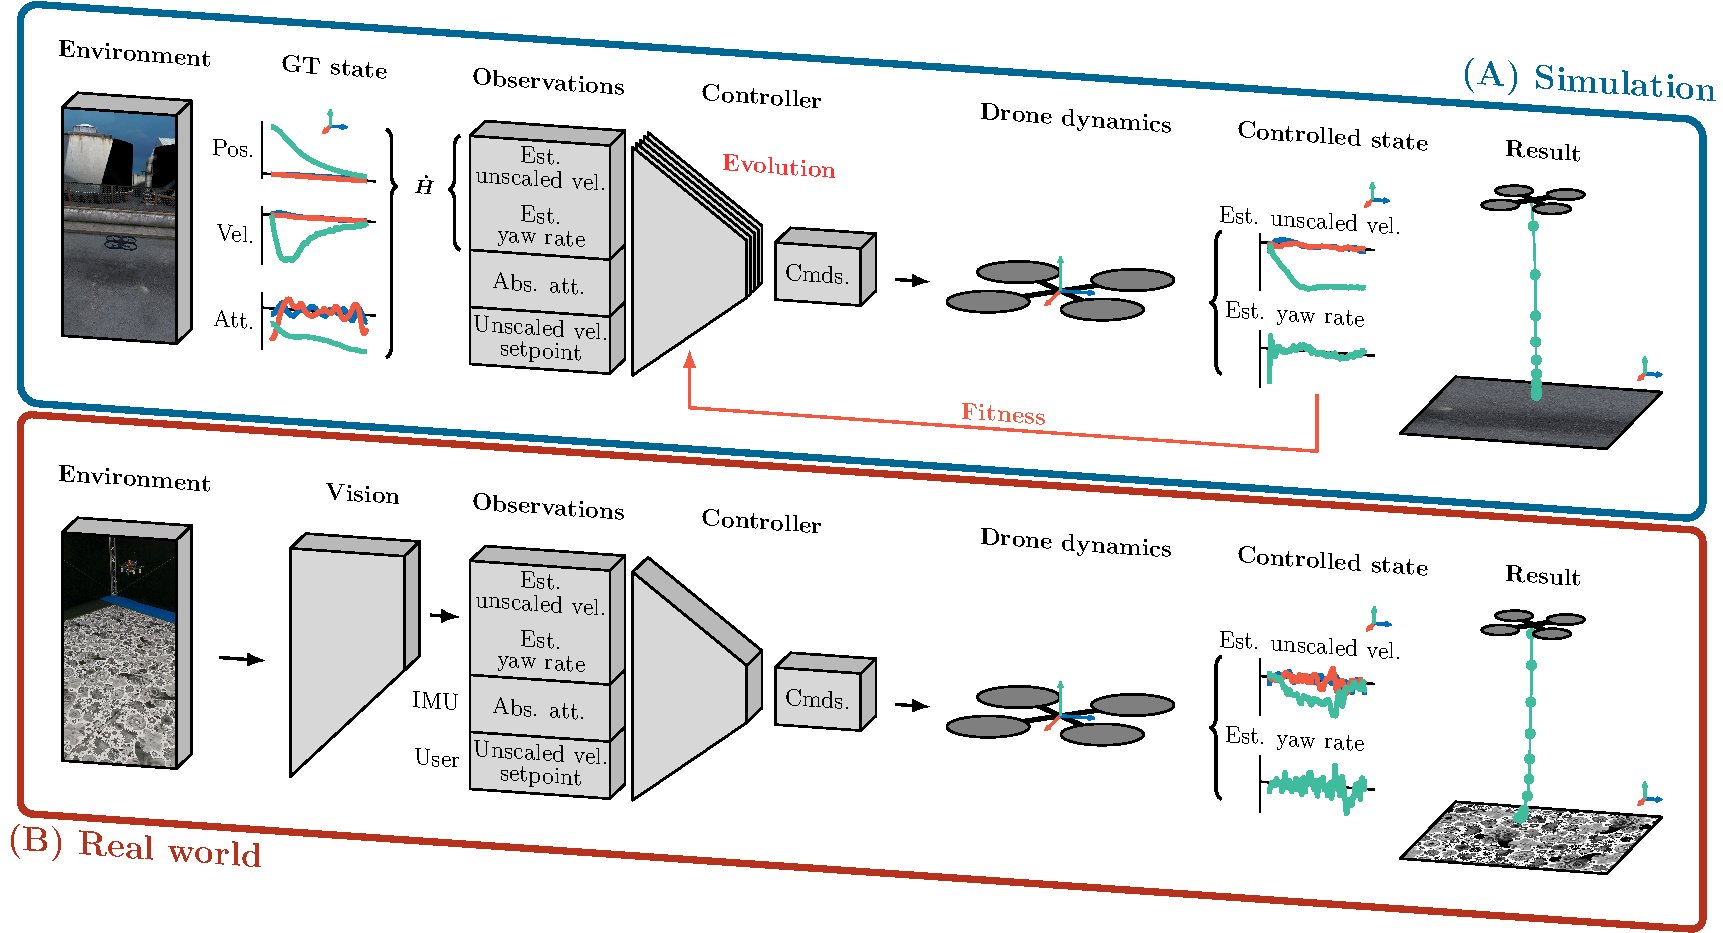
\includegraphics[width=0.975\textwidth]{04_chapters/SR23/figures/fig3-control.pdf}
	\caption{Overview of the control pipeline for simulation and real-world tests. During training in simulation, we construct visual observables (scaled velocities and yaw rate) from ground-truth using the continuous homography transform. The control decoding takes these observables together with roll and pitch and a setpoint to output commands, which control the drone dynamics. We train the controller using evolution based on a fitness signal that quantifies how well the controller can follow setpoints for horizontal and vertical flight. In the real world, we receive flows of the corner ROIs from the vision network, transform these to control commands in a single matrix multiplication, and send these commands to the autopilot.}
	\label{fig:sr_control}
\end{figure*}

\section{Method}

Here, we explain the main components of the proposed fully neuromorphic vision-to-control pipeline, starting with the neuron model of our SNN and how this is trained in a self-supervised fashion using real event camera data. Next, we describe how the vision-based state estimate can be used for navigation, and how we train a controller on top of it. Finally, we discuss the real-world tests and hardware and the performed energy benchmarks.

\subsection{Simulating the on-chip spiking neuron model}

In this study, we utilize a spiking neuron model based on the current-based leaky-integrate-and-fire (CUBA-LIF) neuron, whose membrane potential $U$ and synaptic input current $I$ at timestep $t$ can be written as:
\begin{align}
    U^{t}_{i} &= \tau_U (1 - S^{t-1}_{i}) U^{t-1}_{i} + I^{t}_{i} \\
    I^{t}_{i} &= \tau_I I^{t-1}_{i} + \sum_j w_{ij}^{\text{ff}} S_j^{t} + w_{ii}^{\text{rec}} S_i^{t-1}
\end{align}
where $j$ and $i$ denote presynaptic (input) and postsynaptic (output) neurons within a layer, $S \in \{0, 1\}$ a neuron spike, and $w^{\text{ff}}$ and $w^{\text{rec}}$ feedforward and self-recurrent connections (if any), respectively. The decays (or leaks) of the two internal state variables of this neuron model are learned, and are denoted by $\tau_U$ and $\tau_I$. A neuron fires an output spike if the membrane potential exceeds a threshold $\theta$, which is also learned. The firing of a spike triggers a hard reset of the membrane potential. Note that, in this work, all neurons within a layer share the same decays and firing threshold.

Neurons on the Loihi neuromorphic processor also follow the CUBA-LIF model \cite{davies2018loihi}, however, several considerations must be taken into account to accurately simulate these on-chip neurons. Firstly, the two states variables are quantized in the integer domain. Hence, the parameters associated with these variables are also quantized in the same way: $w\in[-256\ ..\ 256 - \Delta w]$ with $\Delta w$ being the quantization step for the synaptic weights, $\tau_{\{U,I\}}\in[0\ ..\ 4096]$ for the decays, and $\theta\in[0\ ..\ 131071]$ for the threshold. We follow this quantization scheme with $\Delta w=8$ (6-bit weights) in the simulation and training of our neural networks. Secondly, to emulate the arithmetic left (bit) shift operations carried out by the processor when updating the neuron states, we perform a rounding towards zero operation after the application of the decays. Taking these aspects into consideration, we obtain a matching score of 100\% between the simulated and the on-chip spiking neurons. We use quantization-aware training (quantized forward pass, floating-point backward pass) to minimize the performance loss of our SNN when deployed on Loihi.

As surrogate gradient for the spiking function $\sigma$, we opt for the derivative of the inverse tangent~\cite{fang2021incorporating}:
\begin{align}
    \sigma'(x) &= \text{aTan}' = 1/(1 + \gamma x^2) \\
    x &= u - \theta
\end{align}
with $\gamma=10$ being the surrogate width.

\subsection{Four-point parametrization to estimate homography}

Assuming that $\tilde{\boldsymbol{x}}=\left[\boldsymbol{x}^T, 1\right]^T$ and $\tilde{\boldsymbol{x}}'=\left[\boldsymbol{x}'\,^T, 1\right]^T$ are two undistorted corresponding points from a planar scene with pixel array coordinates $\boldsymbol{x}= [x,y]^T$ and $\boldsymbol{x}'= [x',y']^T$ expressed in homogeneous coordinates and captured by a pinhole camera at different time instances, a planar homography transformation is a linear projective transformation that maps $\tilde{\boldsymbol{x}}\leftrightarrow\tilde{\boldsymbol{x}}'$ such that:
\begin{align}\label{eq:homo}
    \lambda 
    \begin{bmatrix}
    x'\\
    y'\\
    1
    \end{bmatrix}
    =
    \boldsymbol{H}
    \begin{bmatrix}
    x\\
    y\\
    1
    \end{bmatrix};\quad \text{with } \boldsymbol{H}=
    \begin{bmatrix}
    h_{11} & h_{12} & h_{13}\\
    h_{21} & h_{22} & h_{23}\\
    h_{31} & h_{32} & h_{33}
    \end{bmatrix}
\end{align}
where $\boldsymbol{H}$ is a 3x3 non-singular matrix, further referred to as the homography matrix, which is characterized by eight degrees of freedom and is defined up to a scale factor $\lambda$, and from which we obtain the normalized form by setting $h_{33}=1$. 

From \eqnref{eq:sr_homo}, we can formulate a system of linear equations for the $k$-th point correspondence:
\begin{align}
    \boldsymbol{A}_k \boldsymbol{h} &= \boldsymbol{b}_k \\
    \boldsymbol{A}_k &=  
    \begin{bmatrix}
    x & y & 1 & 0 & 0 & 0 & -x'x & -x'y \\
    0 & 0 & 0 & x & y & 1 & -y'x & -y'y\\
    \end{bmatrix}\label{eq:4}\\
    \boldsymbol{h} &= 
    \begin{bmatrix}
    h_{11} & h_{12} & h_{13} & h_{21} & h_{22} & h_{23} & h_{31} & h_{32}
    \end{bmatrix}^T\\
    \boldsymbol{b}_k &=
    \begin{bmatrix}
    x' & y'
    \end{bmatrix}^T\label{eq:6}
\end{align}
As shown in \figref{fig:vision}A, our vision network predicts the displacement of the corner ROI pixels in a certain time window. Using this information, we can solve for the components of the homography matrix through:
\begin{equation}
    \boldsymbol{h}=\boldsymbol{A}^{-1}\boldsymbol{b}
\end{equation}
with $\boldsymbol{A}$ and $\boldsymbol{b}$ being the result of the concatenation of the individual $\boldsymbol{A}_k$ and $\boldsymbol{b}_k$ of each point correspondence $\forall\, k\in\{\mathrm{TL},\mathrm{TR},\mathrm{BR},\mathrm{BL}\}$, resulting in a determined system of equations. This approach is referred to as the four-point parametrization of the homography transformation \cite{baker2006parameterizing}, and it has proved to be successful in the event-camera literature for robotics applications \cite{sanket2020evdodgeneta, ozawa2022accuracya}.

Once the homography matrix is estimated, we can estimate a dense (per-pixel) optical flow map as follows:
\begin{align}\label{eq:flow}
    \boldsymbol{u}(\boldsymbol{x}, \boldsymbol{H})=
    \begin{bmatrix}
    u(\boldsymbol{x}, \boldsymbol{H})\\
    v(\boldsymbol{x}, \boldsymbol{H})
    \end{bmatrix}
    =
    \left(\boldsymbol{H}
    \begin{bmatrix}
    x\\
    y\\
    1
    \end{bmatrix}
    \right)_\mathrm{Eucl}
    - 
    \begin{bmatrix}
    x\\
    y
    \end{bmatrix}
\end{align}
which encodes the displacement of pixel $\boldsymbol{x}$ in the time window of $\boldsymbol{H}$. $(\cdot)_\mathrm{Eucl}$ indicates the conversion from homogeneous to Euclidean coordinates.

\subsection{Self-supervised learning of event-based optical flow}

To train our spiking architecture to estimate the displacement of the pixels of the four corner ROIs in a self-supervised fashion, we use the contrast maximization framework for motion compensation \cite{gallego2018unifying, gallego2019focusa}. Assuming constant illumination, accurate optical flow information is encoded in the spatiotemporal misalignments among the events triggered by a moving edge (blur). To retrieve it, one has to learn to compensate for this motion (deblur the event partition) by transporting the events through space and time. Once we get a per-pixel optical flow estimate $\boldsymbol{u}(\boldsymbol{x}, \boldsymbol{H})$ from \eqnref{eq:flow}, we can propagate the events to a reference time $t_{\text{ref}}$ through the following linear motion model:
\begin{equation}\label{eqn:motionmodel}
    \boldsymbol{x}'_i=\boldsymbol{x}_i + (t_{\text{ref}} - t_i)\boldsymbol{
    u}(\boldsymbol{x}_i, \boldsymbol{H})
\end{equation}
where $t$ and $t_\text{ref}$ are normalized relative to the time window between $\boldsymbol{x}$ and $\boldsymbol{x}'$. The result of aggregating the propagated events is the image of warped events (IWE) at $t_{\text{ref}}$, and it having a high contrast indicates good motion compensation/deblurring. 

As loss function, we use the reformulation from \cite{hagenaars2021selfsupervised} of the focus objective function based on the per-pixel and per-polarity average timestamp of the IWE \cite{mitrokhin2018eventbased, zhu2019unsuperviseda}. The lower this metric, the better the event deblurring and hence the more accurate the estimated optical flow. We generate an image of the per-pixel average timestamp for each polarity $p'$ via bilinear interpolation:
\begin{align}\label{eqn:timeimage}
    \begin{aligned}
        T_{p'}(\boldsymbol{x}{;}\boldsymbol{u} |t_{\text{ref}}) &= \frac{\sum_{j} \kappa(x - x'_{j})\kappa(y - y'_{j})t_{j}}{\sum_{j} \kappa(x - x'_{j})\kappa(y - y'_{j})+\epsilon}\\\kappa(a) &= \max(0, 1-|a|)\\
        j = \{i \mid p_{i}=&\ p'\}, \hspace{15pt}p'\in\{+,-\}, \hspace{15pt} \epsilon\approx 0
    \end{aligned}
\end{align}

Following \cite{hagenaars2021selfsupervised}, we first scale the sum of the squared temporal images resulting from the warping process with the number of pixels with at least one warped event:
\begin{equation}\label{eq:scaling}
    \mathcal{L}_{\text{contrast}}(t_{\text{ref}}) = \frac{\sum_{\boldsymbol{x}} T_{+}(\boldsymbol{x}{;}\boldsymbol{u} |t_{\text{ref}})^2 + T_{-}(\boldsymbol{x}{;}\boldsymbol{u} |t_{\text{ref}})^2}{\sum_{\boldsymbol{x}}\left[n(\boldsymbol{x}') > 0\right] + \epsilon}
\end{equation}
where $n(\boldsymbol{x}')$ denotes a per-pixel event count of the IWE.

As in \cite{zhu2019unsuperviseda, paredes-valles2021back, hagenaars2021selfsupervised}, we perform the warping process both in a forward ($t_{\text{ref}}^{\text{fw}}$) and in a backward fashion ($t_{\text{ref}}^{\text{bw}}$) to prevent temporal scaling issues during backpropagation. The total loss used to train our event-based optical flow networks is then given by:
\begin{align}\label{eq:flow_loss}
\mathcal{L}_{\text{contrast}} &= \mathcal{L}_{\text{contrast}}(t_{\text{ref}}^{\text{fw}}) + \mathcal{L}_{\text{contrast}}(t_{\text{ref}}^{\text{bw}})\\
\mathcal{L}_{\text{flow}} &= \mathcal{L}_{\text{contrast}} + \lambda_{\mathcal{L}} \mathcal{L}_{\text{smooth}}\label{eq:final_loss}
\end{align}
where $\mathcal{L}_{\text{smooth}}$ is a Charbonnier smoothness prior \cite{charbonnier1994two} applied in the temporal domain to subsequent per-corner-ROI optical flow estimates, while $\lambda_{\mathcal{L}}$ is a scalar balancing the effect of the two losses. We empirically set this weight to $\lambda_{\mathcal{L}}=0.1$.

As discussed in \cite{hagenaars2021selfsupervised, paredes2023taming}, there has to be enough linear blur in the accumulated input event partition for this loss function to be a robust supervisory signal \cite{gallego2019focusa, stoffregen2019eventa}. Since we process the event stream sequentially, with only a few events being considered at each forward pass, we define the so-called training partition:
\begin{equation}
    \boldsymbol{\varepsilon}^{\text{train}}_{k\rightarrow k+K}\doteq\{(\boldsymbol{\varepsilon}^{\text{inp}}_{i}, \boldsymbol{u}_i)\}_{i=k}^{K}
\end{equation}
which is a buffer that gets populated every forward pass with the input events and their corresponding optical flow estimates. This is illustrated in \figref{fig:vision}A. At training time, we perform a backward pass with the content of the buffer using backpropagation through time once it contains five successive event-flow tuples (25 milliseconds of event data), after which we update the model parameters, detach its states from the computational graph, and clear the buffer. Note that the selection of input and training partition lengths represents deliberate design choices~\cite{valerdi2023insights}, made in alignment with our target execution frequency of 200 Hz, the fact that we do not have direct connectivity between the event camera and the neuromorphic processor, and the statistical attributes of our dataset. We use a batch size of 16 and train until convergence with the Adam optimizer \cite{kingma2017adam} and a learning rate of $1\mathrm{e}{}$-$4$. We validate the quality of the estimated optical flow against the ground-truth optical flow using the average endpoint error (EPE) metric, which is defined as the Euclidean distance between predicted and ground-truth flow values averaged over all pixels in the image:
\begin{equation}
    \mathrm{EPE} = \frac{1}{N}\sum_{i\,\in\,I}^N \lVert \boldsymbol{u}_i - \boldsymbol{u}_i^\mathrm{GT} \rVert
\end{equation}
where $I$ is the set of $N$ pixels in the image, and $u^\mathrm{GT}$ is the ground-truth flow.

\subsection{From a vision-based state estimate to control}

The corner ROI flows $\left[\boldsymbol{u}_\mathrm{TL}^T,\boldsymbol{u}_\mathrm{TR}^T,\boldsymbol{u}_\mathrm{BR}^T,\boldsymbol{u}_\mathrm{BL}^T\right]^T \in \mathbb{R}^{8\times 1}$ resulting from the vision-based state estimation can be used to control the drone. More specifically, we can transform the flows to visual observable estimates~\cite{decroon2013opticflow}, consisting of unscaled velocities $\boldsymbol{\hat{\nu}}^\mathcal{C} \in \mathbb{R}^{3\times 1}$ and yaw rate $\hat{\omega}^\mathcal{C}_z$ in the camera frame $\mathcal{C}$, as follows~\cite{longuet-higgins1980interpretation}:
\begin{align}
    \boldsymbol{u} &=
    \begin{bmatrix}
        -1 & 0 & x & x \\
        0 & -1 & y & -y
    \end{bmatrix}
    \begin{bmatrix}
        \boldsymbol{\nu}^\mathcal{C}\\
        \omega_z^\mathcal{C}
    \end{bmatrix}
    \label{eq:visobs}
\end{align}
where $\boldsymbol{u}$ is the optical flow of a world point with pixel array coordinate $\boldsymbol{x} = [x,y]^T$, and where it is assumed that the scene is static and planar, angles in pitch and roll are small and optical flow is derotated in pitch and roll (meaning the observed flow is only due to translation and yawing). Concatenating \eqnref{eq:visobs} for all four corners of the field of view ($\boldsymbol{u}_k, \boldsymbol{x}_k\, \forall\, k\in\{\mathrm{TL},\mathrm{TR},\mathrm{BR},\mathrm{BL}\}$) allows us to do a least-squares estimation of the unscaled velocities $\boldsymbol{\hat{\nu}}^\mathcal{C}$ and the yaw rate $\hat{\omega}^\mathcal{C}_z$, which can then be transformed to the body frame $\mathcal{B}$. To perform control, we can let a user select visual observable setpoints $\boldsymbol{\nu}_{\mathrm{sp}}^\mathcal{B}$ and $\omega_{z,\mathrm{sp}}^\mathcal{B}$, and use a trained or manually tuned controller to minimize the difference between the estimated visual observables and their setpoints.

\begin{figure}[!t]
	\centering
	\includegraphics[width=\linewidth]{04_chapters/SR23/figures/fig7-merging.pdf}
%	\includegraphics[trim=40 400 0 0, clip, width=0.54\linewidth]{04_chapters/SR23/pdf/fig7-merging.png}
%	\includegraphics[trim=100 0 100 400, clip, width=0.425\linewidth]{04_chapters/SR23/pdf/fig7-merging.png}
	\caption{Merging linear transformations. (\textit{A}) We go directly from output spikes $\boldsymbol{s}$ of the vision network to control commands $\boldsymbol{c}$ in a single linear decoding by multiplying the involved linear transformation matrices. (\textit{B}) The same principle can be applied to connect two separately trained spiking networks in a spiking manner, from spikes $\boldsymbol{s}$ to currents $\boldsymbol{c}$, suitable for neuromorphic hardware.}
	\label{fig:sr_merge}
\end{figure}

Because \eqnref{eq:sr_visobs} is a linear transformation, it can be ``merged'' with other transformations if these are also linear. This holds for the decoding from spikes to corner ROI flows in the vision SNN, meaning that we can use a single linear transformation from spikes to control commands if we use a linear controller. In a similar fashion, we can use this idea to connect separately trained SNNs, merging their linear decodings and encodings. If both are implemented on neuromorphic hardware, this would mean that no off-chip transfer is necessary. \figref{fig:sr_merge} illustrates these concepts.

\subsection{Training control in simulation}

We perform control by linearly transforming the visual observable estimates $\boldsymbol{\hat\nu}^\mathcal{B} \in \mathbb{R}^{3\times 1}$ and $\hat\omega_z^\mathcal{B}$, the drone's absolute roll $\lvert\phi\rvert$ and pitch $\lvert\theta\rvert$ and the unscaled velocity setpoint $\boldsymbol{\nu}^\mathcal{B}_{\mathrm{sp}} \in \mathbb{R}^{3\times1}$ to a control command $\boldsymbol{c} \in \mathbb{R}^{4\times 1}$, which consists of an upward, mass-normalized collective thrust offset from hover $\bar{f}_{0,c}$ in the body frame $\mathcal{B}$, a roll angle $\phi_c$ and pitch angle $\theta_c$, and a yaw rate $\omega^\mathcal{B}_{z,c}$, in order to reach a certain setpoint of unscaled velocities $\boldsymbol{\nu}_{\mathrm{sp}}^\mathcal{B}$ and yaw rate $\omega_{z,\mathrm{sp}}^\mathcal{B}$ (always 0).

The control part is trained separately from the vision part because of the cost of accurately simulating event-based camera inputs (this needs subpixel displacements between frames, hence high frame rate for fast motion). Simulation is done with a modified version of the drone simulator Flightmare \cite{song2020flightmare}. To mimic the output of the vision-based state estimation network, we first compute the ground-truth continuous homography \cite{ma2004invitation,zhong2020direct} from the state of the drone:
\begin{align}
    \boldsymbol{\dot{H}} &= \boldsymbol{K} \left( [\boldsymbol{\omega}^\mathcal{C}]_\times + \frac{1}{p^\mathcal{WC}_z}\boldsymbol{v}^\mathcal{C}(\boldsymbol{e}^\mathcal{W}_{-z})^T \right) \boldsymbol{K}^{-1}
\end{align}
where $\boldsymbol{\dot{H}}$ is the continuous homography, $\boldsymbol{K}$ is the camera intrinsic matrix, $[\boldsymbol{\omega}^\mathcal{C}]_\times \in \mathbb{R}^{3\times 3}$ is a skew-symmetric matrix representing infinitesimal rotations, $p_z^\mathcal{WC}$ is the Z-component of the position vector from the world frame $\mathcal{W}$ to the camera frame $\mathcal{C}$ (representing perpendicular distance from the ground plane to the camera), $\boldsymbol{v}^\mathcal{C}$ is the velocity of the camera, and $\boldsymbol{e}_{-z}^\mathcal{W}$ is the unit vector in the negative Z-direction of the world frame. To obtain angular rates and velocities in the camera frame, we use the camera extrinsics, consisting of a rotation $\boldsymbol{R}^\mathcal{CB}$ and a translation $\boldsymbol{T}^\mathcal{CB}$:
\begin{align}
    \boldsymbol{\omega}^\mathcal{C} &= \boldsymbol{R}^\mathcal{CB} \boldsymbol{\omega}^\mathcal{B}\label{eq:wc} \\
    \boldsymbol{v}^\mathcal{C} &= \boldsymbol{R}^\mathcal{CB} \left( \boldsymbol{v}^\mathcal{B} + [\boldsymbol{\omega}^\mathcal{B}]_\times \boldsymbol{T}^\mathcal{CB} \right)\label{eq:vc}
\end{align}
where the right-hand sides of \eqnreftwo{eq:wc}{eq:vc} are known from the simulator. Next, we use the continuous homography to get the flow of the four corners~\cite{ma2004invitation,zhong2020direct}:
\begin{align}
    \boldsymbol{u}_k &= \left(-\left(\boldsymbol{1} - \tilde{\boldsymbol{x}}_k(\boldsymbol{e}^\mathcal{W}_{-z})^T\right)\boldsymbol{\dot{H}}\tilde{\boldsymbol{x}}_k\right)_\mathrm{Eucl}
\end{align}
where $\boldsymbol{u}_k$ is the flow in Euclidean coordinates, $\boldsymbol{1}$ is the identity matrix, and $\tilde{\boldsymbol{x}}_k = [x_k,y_k,1]^T$ is the projection of the world points in the corners of the field of view onto the pixel array in homogeneous coordinates (so, $\tilde{\boldsymbol{x}}_{\mathrm{BL}} = [0,180,1]^T$ and $\tilde{\boldsymbol{x}}_{\mathrm{TR}}=[180,0,1]^T$, note the difference with respect to \eqnref{eq:visobs}). We add $\mathcal{N}(0, 0.025)$ noise to the flows $\boldsymbol{u}_k$ (based on a characterization of the vision SNN). \eqnref{eq:visobs} is subsequently used to go from flows of the corner ROIs to visual observables in the camera frame, which is then transformed back to the body frame for control. Note that relating camera motion to the motion of points in the image (flow) can equivalently be done with the image Jacobian or feature sensitivity matrix~\cite{corke2011robotics}.

We use a mutation-only evolutionary algorithm with a population size of 100 to evolve the weights of the linear controller matrix $\in \mathbb{R}^{4\times 9}$, whose initial values are drawn from $\mathcal{U}(-0.1, 0.1)$. More specifically, we generate offspring by adding mutations drawn from $\mathcal{N}(0, 0.001)$ to all parameters of each parent and then evaluate the fitness of both parents and offspring. The next generation is comprised of the best 100 individuals, and we repeat this process until convergence (approx. 25k generations). We use Flightmare to assess fitness at flying various visual observable setpoints: every individual is evaluated across a set of 16 setpoints, with each unscaled velocity setpoint $\boldsymbol{\nu}^\mathcal{B}_{\mathrm{sp}}$ having at most one nonzero element $\in \{\pm0.2,\pm0.5,\pm1.0\}$~1/s, skipping the positive setpoints for the Z-direction, and including hover. The yaw rate setpoint is set to $\omega_{z,\mathrm{sp}}^\mathcal{B}=0$ for all. Each setpoint is repeated ten times, meaning a total of 160 evaluations per individual. Fitness $F$ is computed as:
\begin{align}
    F &= \frac{1}{N_\mathrm{eval}} \sum_{i \in N_\mathrm{eval}} \sum_{j \in N_{\mathrm{steps}}} \boldsymbol{w} \cdot \left( \boldsymbol{\nu}^\mathcal{B}_{\mathrm{sp},i} -
    \begin{bmatrix}
        \hat{\nu}_x^\mathcal{B}\\
        \hat{\nu}_y^\mathcal{B}\\
        \nu_z^\mathcal{W}
    \end{bmatrix}_j\,
    \right)^2 + \left(\hat{\omega}_z^\mathcal{B}\right)^2
\end{align}
Here, $N_{\mathrm{eval}}$ is the number of evaluations, $N_\mathrm{steps}=1000$ is the number of steps per evaluation, and $\boldsymbol{w}=[1, 1, w_z]^T$ is a vector weighing the fitness for different axes, where we set $w_z=10$ for setpoints where $\nu^\mathcal{B}_{z,\mathrm{sp}}=0$. Note that, for the Z-direction, we use the ground-truth unscaled velocity in the world frame $\nu_z^\mathcal{W}$ instead of the one in the body frame, as the latter is zero in the case of the drone ascending or descending at a slope equal to its attitude, and would hence go unpunished, leading to extra vertical drift. Furthermore, if the simulated drone goes out of bounds or crashes before the end of an evaluation, it will be reset without any additional fitness penalty.

We use domain randomization~\cite{tobin2017domain} to obtain a more robust controller and reduce the reality gap: for each of the ten repeats, a random constant bias $\mathcal{U}(-0.001, 0.001)$~rad is added to the absolute pitch and roll received by the control layer. This bias is shared among the population to keep things fair. Furthermore, for each of the 160 evaluations per individual, we randomly vary the initial position $\boldsymbol{p}^\mathcal{WB} = [0,0,2]^T + \mathcal{U}^{3\times1}(-1, 1)$ m (except for horizontal flight, where we fix $p^\mathcal{WB}_{z}$ to 1.5~m, due to the linear nature of the controller we have here, as explained later), initial velocity $\boldsymbol{v}^\mathcal{WB} \sim \mathcal{U}^{3\times1}(-0.02, 0.02)$~m/s, initial attitude quaternion $\boldsymbol{q}^\mathcal{WB} \sim \mathcal{U}^{4\times1}(-0.02, 0.02)$ (normalized), and initial angular rates $\boldsymbol{\omega}^\mathcal{B} \sim \mathcal{U}^{3\times1}(-0.02, 0.02)$~rad/s.

We modify Flightmare to include drag $\boldsymbol{f}_\mathrm{drag}$ occurring as a result of translational motion, and we take it to be acting in the so-called ``flat-body'' frame $\mathcal{B'}$, which is the body frame rotated by the roll and pitch of the drone, such that the Z-axis is aligned with the world Z-axis. Following~\cite{dewagter2022sensing}, we use a drag model that is linear with respect to velocity in X and Y, but using a drag coefficient $k_{v,x}=k_{v,y}=0.5$. This results in the following:
\begin{align}
    \boldsymbol{f}_\mathrm{drag}^\mathcal{B} &= -\boldsymbol{R}^\mathcal{BB'}
    \left(
    \begin{bmatrix}
        k_{v,x} \\
        k_{v,y} \\
        0
    \end{bmatrix}
    \circ \boldsymbol{R}^\mathcal{B'B}\boldsymbol{v}^\mathcal{B}
    \right)
\end{align}

The outputs of the linear controller $\boldsymbol{c}\in \mathbb{R}^{4\times1}$ are clamped to $[-1,1]$ and fed to different parts of the cascaded low-level (thrust, attitude and rate) controllers. To accommodate some of the shortcomings of the linear controller, we compensate thrust for the attitude of the drone.

All dynamics equations are integrated with 4$^{\mathrm{th}}$-order Runge-Kutta with a timestep of 2.5~ms. The frequency of the simulation is 50~Hz. %All remaining details can be found in the Supplementary Methods.

% \subsection{From simulation to the real world}

% We achieve successful sim-to-real transfer through several strategies. One is domain randomization~\cite{tobin2017domain}, which we do by adding noise to the observed flows, through a random bias on the attitude estimate, and by varying the initial conditions of the simulated quadrotor. Another is abstraction~\cite{scheper2017abstraction}, which we do by making use of low-level controllers to go from thrust and attitude to rotor speeds and by calibrating the attitude and hover thrust biases before each flight to make sure they are small/zero (as in the simulator). Finally, we smooth (low-pass filter) and scale the computed visual observables and tune the gains scaling the control layer outputs in the real world.

% \eqnref{eq:visobs} is used to transform the flows of the corner ROIs coming from the vision network into visual observables (unscaled velocities $\boldsymbol{\hat{\nu}}^\mathcal{B}$ and yaw rate $\hat{\omega}^\mathcal{B}_z$), absolute roll $\lvert\phi\rvert$ and pitch $\lvert\theta\rvert$ are taken from the drone's accelerometers, and the unscaled velocity setpoint $\boldsymbol{\nu}^\mathcal{B}_{\mathrm{sp}}$ is provided by the user. The yaw rate setpoint $\omega_{z,\mathrm{sp}}^\mathcal{B}=0$ is fixed.

% Extra experiments were performed by connecting the vision network to a hand-tuned proportional-integral (PI) controller. All remaining details can be found in the Supplementary Methods.

\subsection{Hardware setup}

Real-world experiments were performed with a custom-built quadrotor carrying the event-based camera (DVS 240), a single-board computer (UP Squared) and a neuromorphic processor (Intel Kapoho Bay with two Loihi neuromorphic research chips). A high-level overview can be found in \figref{fig:pipeline}, with all components are listed in \tabref{tab:components}. We use PX4 as autopilot firmware, and ROS (Robot Operating System) for communication. More specifically, events coming from the event-based camera are passed to the UP Squared over USB (Universal Serial Bus) using ROS1. These events are processed (downsampling, cropping, limiting to 90 per image corner ROI) on the UP Squared, and sent as spikes to the vision network running on the Kapoho Bay over USB. After processing, the output spikes are sent back over USB to the UP Squared, where they are decoded into flows for each corner ROI. The ROI flows are then published by a ROS1 node, and sent to ROS2 over a ROS1-ROS2 bridge. The linear controller (or PI controller, for that matter) and the processing around it, running as a ROS2 node, takes the ROI flows together with the attitude estimate coming from PX4 (IMU) and the ego-motion setpoint provided by the user, and outputs the control command. This command is then sent over ROS2 to PX4, and processed by the low-level controllers there. ROS2 makes use of RTPS (real-time publish-subscribe) for communication, which allows for high-frequency and high-bandwidth messaging between the UP and PX4, meaning our entire pipeline can run at 200~Hz\textemdash approximately the frequency of PX4's attitude controller. This attitude control frequency was a major driver for our choice to run the neuromorphic pipeline at the same frequency. This choice also depended on various other factors, ranging from the trade-off between a fast execution frequency and good optical flow estimation to the limitations of the spike interfacing over USB. Importantly, a 5~ms event window turned out to give accurate optical flow estimates, as well as a very fast execution frequency (see Supplementary Methods). Moreover, this frequency can be attained reliably, as Table \ref{tab:energy} shows that Intel's Loihi inference time is consistently faster than 5~ms. For position control between test runs, and as failsafe, we use an OptiTrack motion capture system.

% We estimate power required for hover flight by flying with a fully charged battery until a certain voltage, keeping track of time, and estimating spent mAh using the value from the charger. During this flight, the UP Squared is powered on (needed for control), and we estimate a power consumption of 277~W. Subtracting the estimated 18~W for the UP Squared makes the 259~W for the remaining components in \tabref{tab:components}. For the Kapoho Bay, we use the numbers from the performed energy benchmark, given that running power is almost equal to idle power. We get power estimates for the UP Squared (version UPS-APLX7-A20-0864) and DVS 240 from online available datasheets.

\begin{table}[!t]
	\centering
	\resizebox{0.85\linewidth}{!}{%
	\begin{tabular}{@{}llrr@{}}
		\thickhline
		\thickhline
		Component     & Product & Mass [g] & $\sim$Power [W]               \\ \midrule
		Frame                  & GEPRC Mark 4 225~mm &  \multirow{5}{*}{508} & \multirow{5}{*}{259}           \\
		Motor                  & Emax 2306 Eco II Series & &        \\
		Propellor              & Ethix S5 5~inch  & &               \\
		Flight Controller      & Pixhawk 4 Mini  &   &              \\
		ESC                    & SpeedyBee 45A BL32 4in1  &     &   \\ \midrule
		Battery                & Tattu FunFly 1800mAh 4S  & 195   &  -  \\ \midrule
		Single-board computer  & UP Squared ATOM Quad Core 08/64  & 202 & 18 \\ \midrule
		Event-based camera           & DVS 240  & 27     &      1\\ \midrule
		Neuromorphic processor & Intel Loihi, Kapoho Bay form factor  &  62   &   1\\ 
		\thickhline
		\thickhline
	\end{tabular}}
	\caption{List of hardware components used for the real-world test flights.}
	\label{tab:sr_components}
\end{table}

\subsection*{Energy benchmark}

Energy benchmarks for Loihi were performed on a Nahuku board (host machine: Intel Xeon Platinum 8280 CPU at 2.7 GHz, 126 GB RAM, Ubuntu 20.04, NxSDK 1.0.0), which contains 32 Loihi chips, as Kapoho Bay does not support energy probing. These (software) probes report a variety of power measurements, as well as execution times. Following the documentation, static power is due to transistor leakage, dynamic power is due to switching, idle power is measured while the embedded CPU cores on Loihi are still clocked but the neuromorphic are inactive, and total/running power is due to all components together. Kapoho Bay does support probing execution times, which we used to confirm that these are almost identical between Nahuku and Kapoho Bay. Furthermore, documentation states that Nahuku shuts down unused chips, meaning it can emulate energy consumption of a Kapoho Bay (which has two chips) with minimal overhead. Still, these benchmarks are not very representative of actual use on a drone, because that involves receiving and processing streaming data in an online fashion, whereas here all data is loaded to memory beforehand, and then processed as quickly as possible. Therefore, what these benchmarks represent is not the energy consumption and execution speed of the whole pipeline, but rather that of the network alone, without any bottlenecks and influences due to I/O and preprocessing. This also explains the much higher execution frequencies of Loihi with respect to real world tests, where this was always around 200~inf/s.

On Jetson Nano, we simulate the SNN and ANN in PyTorch (ARM Cortex-A57 CPU at 1.43 GHz, 4 GB RAM, Ubuntu 20.04, PyTorch 1.12.0). Jetson Nano has two power modes: a low-power (5W) mode, and a max-power (10W) mode, the difference being the number of active CPU cores (two versus four) and the frequencies of the active CPU and GPU cores. Power consumption was measured using the tegrastats utility, and execution time was measured in Python code. Note that the split between static and dynamic power cannot be made here as these are not available as measurements. Idle power is measured for a period of time after running the benchmarks.

\subsection*{Statistical analysis}

Unless mentioned otherwise, figures and tables show individual runs without any statistical method applied. Reported EPEs (as in \tabref{tab:AEEchanges}) are averaged over sequences in the test dataset. Reported drifts (as in Tables \ref{tab:simsnndrifts}, \ref{tab:realsnndrifts} and \ref{tab:realpidrifts}) are averaged over all runs in a certain flying direction.

For investigating the influence of the tether on the drone dynamics (see Supplementary Results), we performed a Z-test with sampling distributions created using bootstrapping~\cite{cohen1995empirical} and a confidence interval of 95$\%$ was used to determine significance.

\section{Experiments}

Because of the split between the vision and control parts of the pipeline, we can evaluate their performance separately. The estimated corner ROI flows of the vision part are compared against ground truth data obtained from a motion capture system, while the control part is evaluated in simulation. Connecting vision and control together, we then demonstrate the performance of our fully neuromorphic vision-to-control pipeline through real-world flight tests. To further illustrate the robustness of our vision-based state estimation, we perform real-world tests with changing setpoints, and tests in various lighting conditions. Lastly, we compare energy consumption against possible on-board GPU solutions.

\begin{figure*}[!h]
	\centering
	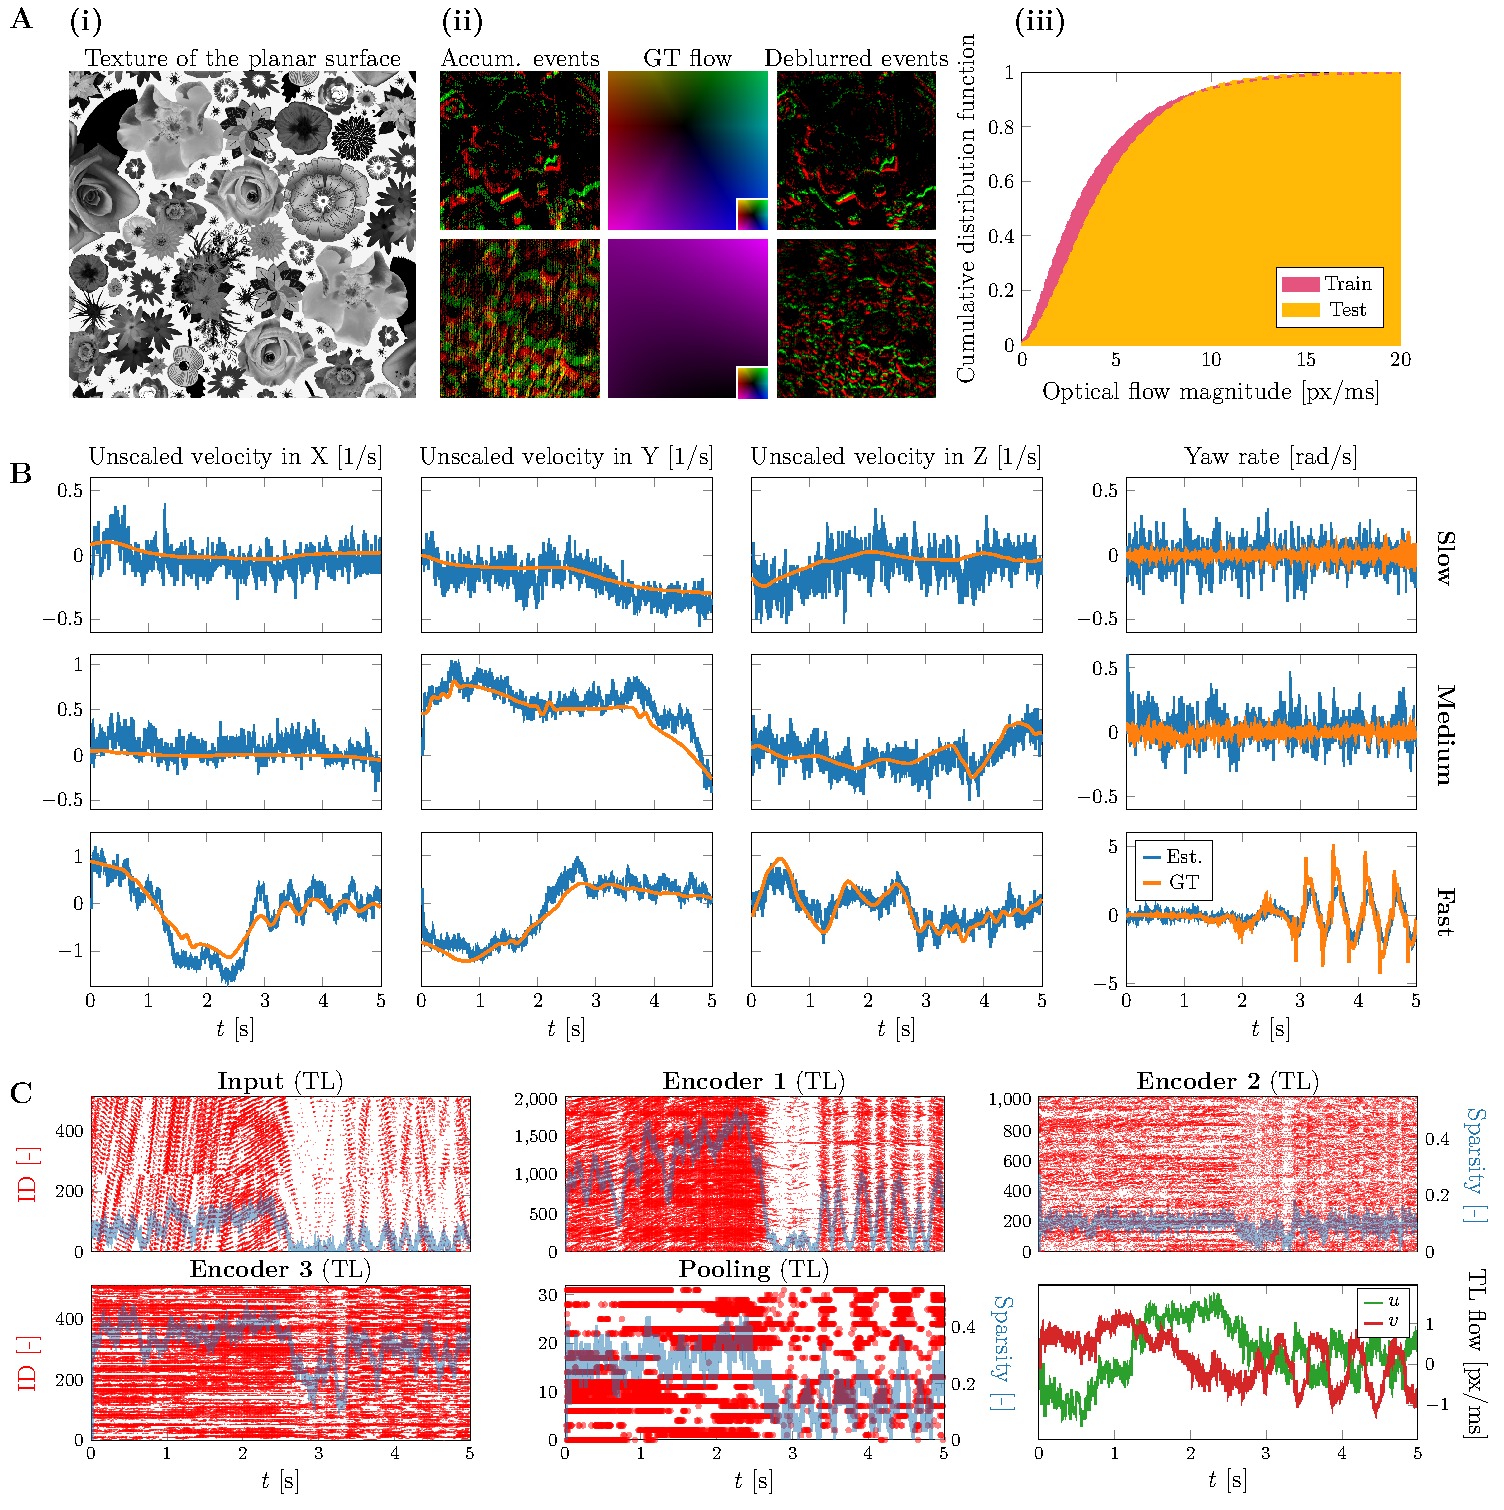
\includegraphics[width=\textwidth]{04_chapters/SR23/figures/fig4-vision-results.pdf}
	\caption{Overview of results for the vision-based state estimation. (\textit{A}) Characteristics of the dataset for estimating planar optical flow. \emph{Left:} Grayscale flower texture used to cover the floor. \emph{Center:} Accumulated event windows showing the blur arising from motion, ground truth flow fields as determined with a motion tracking system and based on a flat floor assumption (only for evaluation), and the result when using the flow fields to deblur the event windows (only for illustration). \emph{Right:} Ground-truth optical flow distributions for the training and test datasets. (\textit{B}) Comparison of estimated and ground-truth visual observables for sequences with different motion speeds (slow, medium, fast). (\textit{C}) Network activity resulting from the events in the top-left-corner ROI in the fast motion sequence.}
	\label{fig:sr_vision_results}
\end{figure*}

\subsection{Robust vision-based state estimation}

\begin{table*}[!t]
	\centering
	\resizebox{0.95\textwidth}{!}{%
		\begin{tabular}{@{}lrrrrr@{}}
			&&&&&\multicolumn{1}{r}{$\cdot 10^{-2}$}\\
			\thickhline
			\thickhline
			&  Full image   & +2x Down. & +Corner ROI crop & +Limit events & +Loihi quant. \\ \midrule
			Conv-GRU ANN                      & 5.88    & 5.56      & 5.61       & 5.72    & -       \\ \midrule
			Conv-RNN SNN                      & 7.92    & 7.89      & 7.91       & 6.97    & 6.96      \\ \midrule
			Self-RNN SNN (ours)                      & 10.79    & 9.80      & 8.22       & 7.71    & \textbf{8.34}      \\ 
			\thickhline
			\thickhline
		\end{tabular}
	}
	\caption{Quantitative comparison between different vision architectures. Bottom right corner, in bold, indicates the final architecture. Architecture choices (row-wise) and design decisions (column-wise) impact test performance in terms of the average endpoint error (EPE$\downarrow$, lower is better). Baseline architectures feature the same feedforward connectivity pattern as ours, but vary the neuron model and the type of recurrent connections.}
	\label{tab:sr_AEEchanges}
\end{table*}

To prevent reality-gap issues when simulating an event-based camera, we trained and evaluated the vision part of our pipeline using real-world event sequences recorded with the same platform (drone and downward-facing event-based camera) and in the same indoor environment (static and planar, constant illumination). This dataset consists of approximately 40 minutes of event data, which we split into 25 minutes for training and 15 for evaluation, and its motion distributions are shown in \figref{fig:vision_results}A. In addition to the visual data, the ground truth pose (position and attitude) of the drone over time was provided at a rate of 180 Hz, and was used solely for evaluation. Examples of this ground truth, which can be converted to dense optical flow using the camera calibration, are shown in \figref{fig:vision_results}A alongside the floor texture of the indoor environment. %Note that this dataset is available with the Supplementary Material of this work. Furthermore, to demonstrate that using the same texture for training and evaluation does not lead to overfitting (and resulting degraded control performance), we performed additional experiments with different types of texture that can be found in the Supplementary Material.

We trained our vision SNN with the self-supervised contrast maximization framework from \cite{hagenaars2021selfsupervised} and a quantization-aware training routine that simulates the neuron and synapse models in the target neuromorphic hardware. Afterwards, we evaluated the performance of our spiking network on the task of planar event-based optical flow estimation using sequences with varying amounts of motion. Qualitative results are presented in \figref{fig:vision_results}B, where the estimated visual observables (unscaled velocities and yaw rate, constructed from the estimated optical flow vectors at the image corner ROIs) are compared to their ground-truth counterparts. These results confirm the validity of our approach. Despite the architectural limitations of the proposed solution (for instance, lower resolution due to binary activations, limited field of view, only self-recurrency, weight and state quantization) and the fact that it does not have access to ground-truth information during training, it was able to produce optical flow estimates that accurately capture the motion encoded in the input event stream (the ego-motion of the camera), even for the fast rotation of approximately 4~rad/s at the end of the shown sequence. Note that, similarly to any other optical-flow-based state-estimation solution, our SNN is subject to the aperture problem not only due to the limited receptive field of the corner ROIs but also because of the use of event cameras as vision sensors \cite{gallego2020eventbased}.

In \figref{fig:vision_results}C, we show the internal spiking activity of our vision SNN as it processes the top-left corner ROI from the fast sequence shown in \figref{fig:vision_results}B, along with the decoded optical flow vectors. These qualitative results provide insight into the type of processing carried out by the proposed architecture, which is spike-based and therefore sparse and asynchronous. Notably, despite the rapid motion in the input sequence, all layers of the SNN maintained activation levels below 50\% of the available neurons. Note that the network was not explicitly trained to promote sparse activations, but could perhaps be rendered even more energy efficient by including sparsity measures in the loss function. Furthermore, we can distinguish layers with activity levels that are highly correlated with the input activity (encoder 1 and pooling), and layers that rely on their explicit recurrent connections to maintain activity levels that are relatively independent of the input statistics (encoder 2 and encoder 3). This observation could be the starting point for a future investigation into how this type of network determines optical flow (as in~\cite{dejong2021neural}).

In \tabref{tab:AEEchanges}, we provide a quantitative comparison of our solution with other similar recurrent architectures (that are not compatible or do not fit in the Intel Kapoho Bay), based on the average endpoint error (EPE, the Euclidean distance between predicted and ground-truth optical flow vectors averaged over all pixels in the image). This evaluation not only demonstrates the accuracy of our spiking network, but also assesses the effect of each mechanism that was incorporated into the pipeline to achieve a solution that could be deployed on Loihi at the target frequency of 200~Hz (downsampling the image space, only processing the events from the corner ROIs, limiting the maximum number of processed events per corner, and adding quantization; see also the Supplementary Methods). Several observations could be made. Firstly, the ANN outperformed its spiking variants by a large margin. This is likely due to the higher resolution of the floating point activations and the direct relation between the backpropagation gradient and the output error. Secondly, self-recurrency (Self-RNN) was the weakest form of explicit recurrency among those tested. The other networks seemed to successfully exploit their capability of representing more complex temporal functions.
Thirdly, deploying one architecture to each image corner ROI instead of processing the entire image space at once was beneficial for our architecture (lowering the EPE from 9.80 to 8.22), but had a slight detrimental effect on the baselines. This may be due to the dataset containing ample texture on the floor. A dataset with much less texture might have shown a different result. Fourthly, limiting the number of events that can be processed at once to 90 per corner ROI was also helpful for the evaluated SNNs, as it helped reduce the internal activity levels. Lastly, the incorporation of the Loihi-specific weight and state quantization led to an error increase for our architecture.

\begin{figure*}[!t]
	\centering
	\vspace{10pt}
	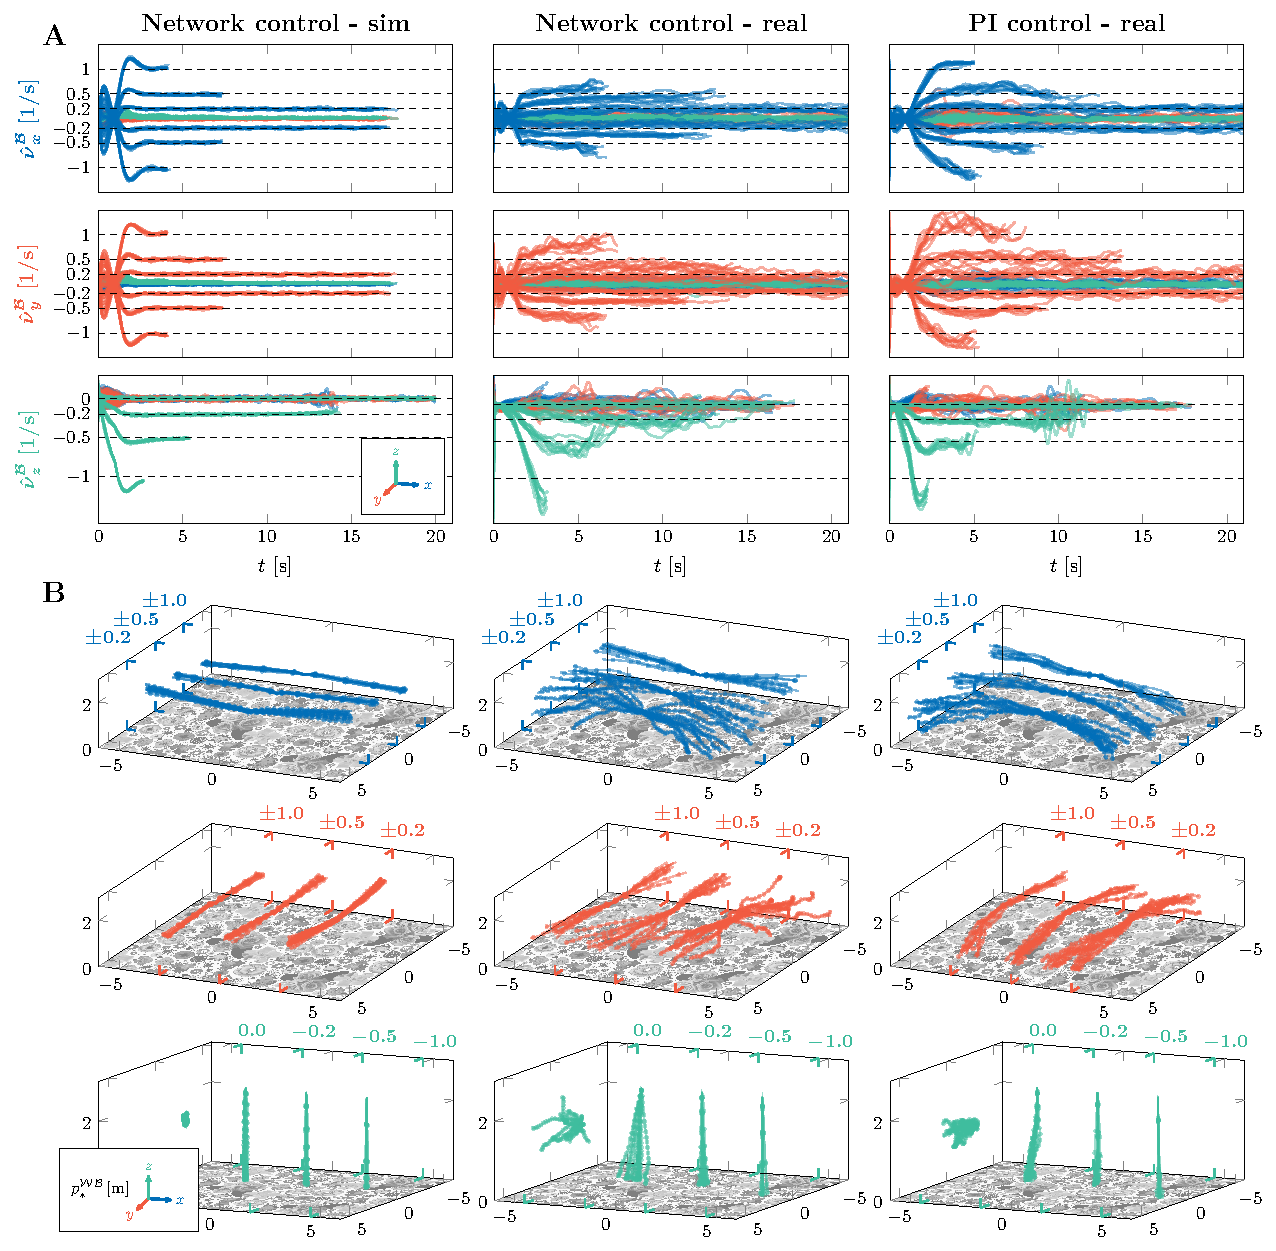
\includegraphics[width=\textwidth]{04_chapters/SR23/figures/fig5-simnetpi-results.pdf}
	\caption{Comparison of results obtained in simulation and during real-world flight tests. (\textit{A}) Estimated scaled velocities for 16 different setpoints in three axes, across three scenarios: linear network controller in simulation and the real world, and a hand-tuned proportional-integral (PI) controller in the real world. Real-world tests use the vision network to obtain visual observable estimates. Setpoints are nonzero in one direction, indicated with dashed lines. Rows represent the different motion axes. (\textit{B}) 3D world position trajectories for the same flight tests. Each cube in (\textit{B}) matches the plot in the corresponding location in (\textit{A}).}
	\label{fig:sr_results1}
\end{figure*}

\subsection{Control through visual observables: From sim to real}

Separately from the vision part, we trained and evaluated the control part of our pipeline. Due to limitations in the hardware setup (see Materials and Methods), this is a linear mapping from a visual observable estimate, absolute roll and pitch and a visual observable setpoint to thrust and attitude commands. The visual observable estimate is made up of unscaled velocity $\boldsymbol{\hat{\nu}}^\mathcal{B}$ and yaw rate $\hat{\omega}^\mathcal{B}_z$; the visual observable setpoint consists of the corresponding setpoints in unscaled velocity $\boldsymbol{\nu}^\mathcal{B}_{\mathrm{sp}}$ and yaw rate $\omega^\mathcal{B}_{z,\mathrm{sp}}$.
A population of these linear mappings was evolved in simulation for a set of 16 unscaled velocity and yaw rate setpoints. Each unscaled velocity setpoint $\boldsymbol{\nu}^\mathcal{B}_{\mathrm{sp}}$ had at most one nonzero element $\in \{\pm0.2,\pm0.5,\pm1.0\}$~1/s. In other words: they represented hover, vertical flight in the form of landing at three speeds (no ascending flight), and horizontal flight in four directions at three speeds. Unless mentioned otherwise, the setpoint for yaw rate $\omega^\mathcal{B}_{z,\mathrm{sp}} = 0$. \figref{fig:results1} shows the performance of the evolved linear network controller in simulation in terms of the estimated unscaled velocities $\boldsymbol{\hat{\nu}}^\mathcal{B}$ (\figref{fig:results1}A) and the world position $\boldsymbol{p}^\mathcal{WB}$ over time (\figref{fig:results1}B) for all setpoints. The control performance was satisfactory; The controller reached the setpoint in all cases, and was capable of keeping the unscaled velocities for the non-flight direction close to zero. Especially for $\nu_{*,\mathrm{sp}}^\mathcal{B}=\pm1.0$~1/s, some overshoot was witnessed, but this could be expected given that this is a linear mapping without any kind of derivative control.

\figref{fig:results1} furthermore shows the results obtained by deploying this controller in the real world, and replacing the ground-truth visual observables with those estimated by the vision network (also see Movie S3). Overall, the results demonstrated successful deployment of the fully neuromorphic vision-to-control pipeline. Looking at the unscaled velocity plots for the different setpoints, we see that these became less noisy for higher setpoints and faster flight, as can also be seen from the 3D position plots. This is due to the fact that the signal-to-noise ratio of the vision-based state estimation increased with motion magnitude (little motion means most events are due to noise, as can be seen in \figref{fig:vision_results}). Also, the inertia of the drone provided some stability at higher speeds. Nevertheless, apart from several setpoints (for example, landings, $\nu^\mathcal{B}_{\{x,y\},\mathrm{sp}} = \pm0.2$~1/s), the controller was not always able to reach the desired setpoint: the steady-state error looked to be proportional to the setpoint magnitude. This could be attributed to the fact that although the controller is a linear mapping, the relationship between attitude angle and resulting forward/sideways velocity is nonlinear (especially at larger attitude angles), and additionally affected by drag.
Providing absolute attitude input to the network, and simulating the drag (as in \cite{dewagter2022sensing}) during training turned out not to be enough to compensate, and small errors were accumulated over time. Furthermore, there can be mismatches between the dynamics of the simulated drone (body characteristics, motor dynamics) with which the controller was trained and the real drone on which the flight tests were performed, even though we abstracted the control outputs to attitude commands. Lastly, inaccuracies of the drag model can also be a source of error (in this case, it seems that drag was higher in reality than in simulation). A linear or proportional controller, such as we have here, cannot integrate all these small errors into an additional control signal that compensates for them, leaving a steady-state error. The resulting drift in position and yaw for all runs in \figref{fig:results1} were quantified in the Supplementary Results.
 
Lastly, \figref{fig:results1} shows the results obtained by connecting a hand-tuned proportional-integral (PI) controller to the vision-based state estimation (also see Movie S4). We compared this to the linear network controller. Looking at all directions and setpoints, we see that the PI controller reaches the setpoint faster than the network controller. For horizontal flight, the network controller was not at all able to reach the setpoint $\nu^\mathcal{B}_{\{x,y\},\mathrm{sp}} = \pm1.0$~1/s and only just in the case of $\pm0.5$~1/s, supposedly due to the limitations of linear control. The PI controller did not have this problem, as it could increment its control command to eliminate the steady-state error. For vertical flight, both the network and the PI controller had quite some overshoot for $\nu^\mathcal{B}_{z,\mathrm{sp}} = -1.0$~1/s. This had to do with the fact that at such speeds from such heights (2.5~m), the drone barely reached the setpoint before reaching the ground, and therefore had little time to compensate for any overshoot (see \figref{fig:results1}A, PI controller for $\nu^\mathcal{B}_{z,\mathrm{sp}} = -0.5$~1/s, for which overshoot was similar but is corrected shortly after).

\subsection{Other examples of versatility and robustness}

\begin{figure*}[!t]
	\centering
	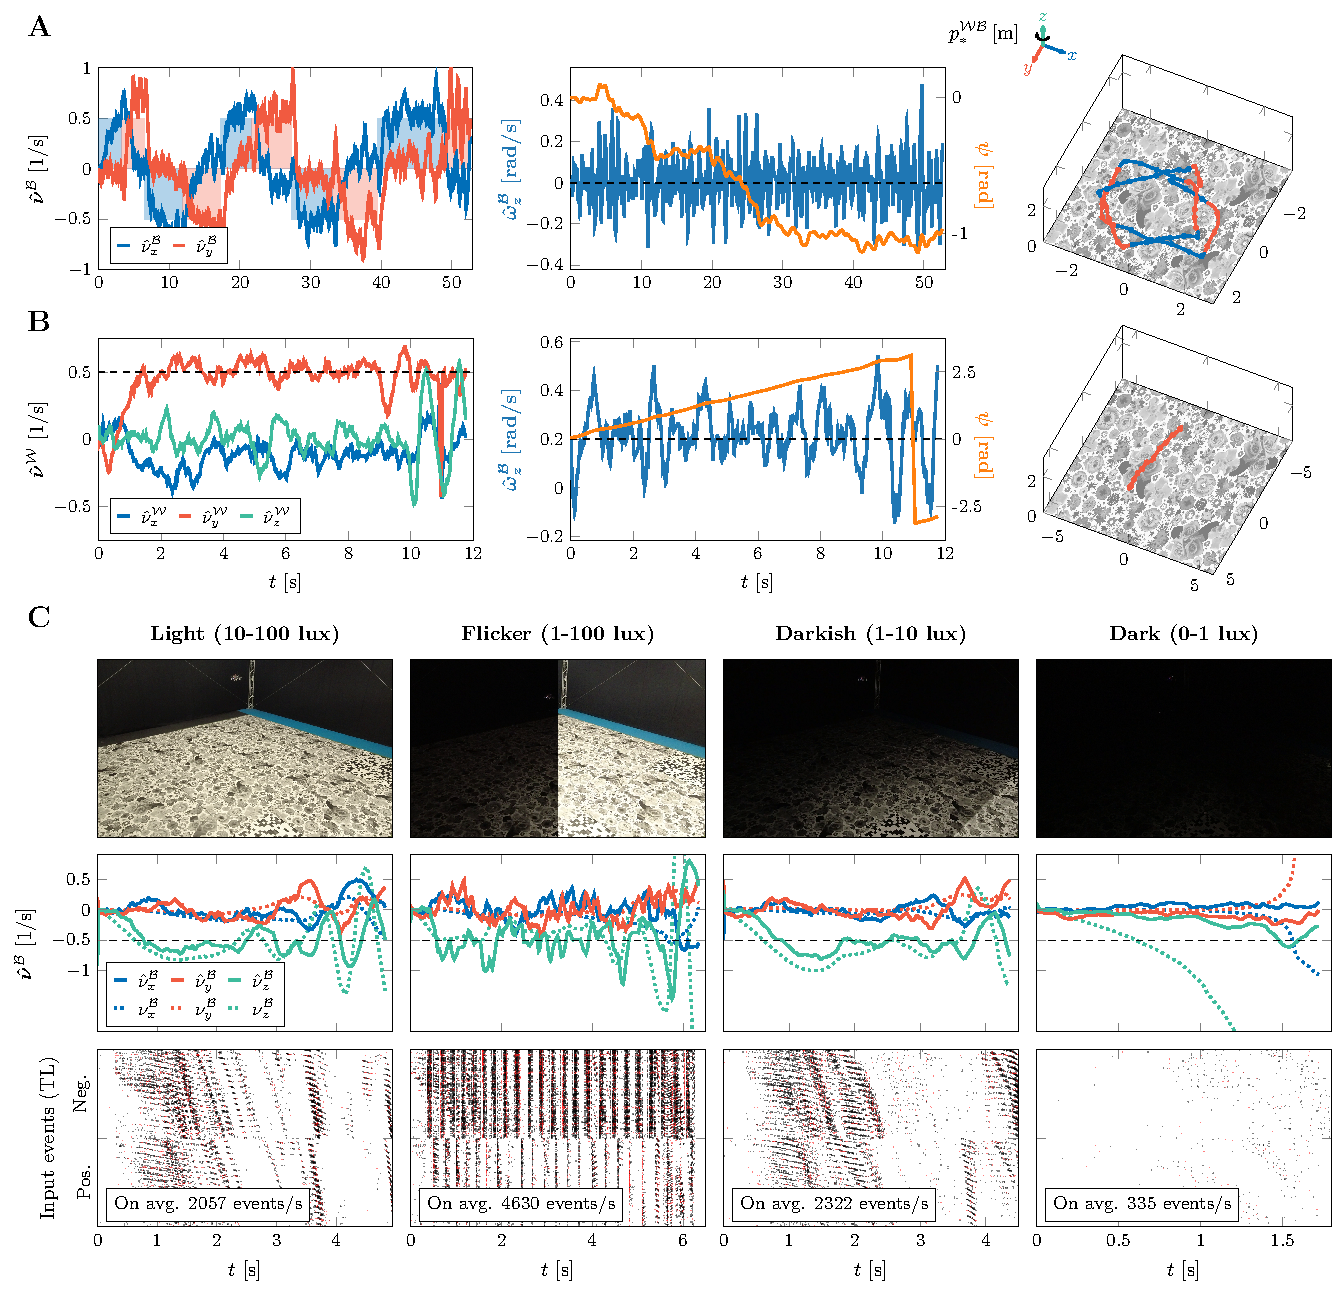
\includegraphics[width=\textwidth]{04_chapters/SR23/figures/fig6-pispecial-results.pdf}
	\caption{Additional results with vision network and proportional-integral (PI) controller. (\textit{A}) \textit{Top row}: alternating setpoints in X and Y (shaded areas) in order to fly a square. \textit{Bottom row}: rotating the scaled velocity setpoint by the yaw angle, while maintaining a yaw rate setpoint of 0.2 rad/s (dashed line), leads to the drone spinning around its Z-axis while flying in a straight line. (\textit{B}) Landing experiments with different lighting conditions. While flickering lights lead to many more events, visual observable estimates (and hence control) only diverge when it is so dark that there are almost no events.}
	\label{fig:sr_results3}
\end{figure*}

Although our main goal is to show a functional fully neuromorphic vision-to-control pipeline, for a broader applicability of this technology it is informative to study the pipeline's robustness and versatility to conditions not encountered during learning. \figref{fig:results3} shows the results for these tests for the combination of the vision-based state estimation and linear network controller. \figref{fig:results3}A displays the user alternating through different unscaled velocity setpoints in X and Y (while keeping yaw constant) in order to let the drone fly a square. Apart from one section, the controller was able to reach the desired setpoint quite quickly, allowing for sharp corners, while keeping yaw drift small (0.06~rad).

Furthermore, we have tested the robustness to lighting conditions for maneuvers in different directions. Here, we show the results of these experiments for the landing maneuver (see Supplementary Results for the other directions). Because landing involves a wider range of visual motion magnitudes than horizontal flight (flow inversely proportional to height), it allowed us to better see the effect of lower-light conditions. Furthermore, divergence-based landings inherently lead to oscillations~\cite{decroon2016monocular}, which makes for a more challenging scenario in the case of flickering lights. \figref{fig:results3}B shows landing with divergence $\nu^\mathcal{B}_{z,\mathrm{sp}}=-0.5$~1/s for various lighting conditions (quantified with lux measurements). With these experiments we aimed to investigate the robustness of the approach to wildly varying event statistics. For instance, in a darker environment, contrasts are less visible, which means that motion will generate many fewer events and that there will be more spurious, noisy events\textemdash similar to our own human vision when we walk in the dark. When lights are switched on and off, this generates massive numbers of events that are unrelated to motion, hence violating the brightness constancy assumption underlying optical flow determination. The events for the top left corner ROI are shown in \figref{fig:results3}B. The results in the light and darkish settings look alike, but flickering lights led to a large increase in events, and the darkest setting gave almost no events. As \figref{fig:results3}B shows, despite the challenging light conditions, the controller was able to track the setpoint (black dashed line) quite well, and the estimated unscaled velocities approximated their ground truths. Only the darkest setting posed a real problem for the state estimation: in that case, the estimated unscaled velocities $\boldsymbol{\hat{\nu}}^\mathcal{B}$ diverged too much from the ground truth unscaled velocities $\boldsymbol{{\nu}}^\mathcal{B}$ to perform a successful landing. %For comparison, the flickering, darkness, and squares experiments have also been performed with the PI controller, which can be found in the Supplementary Results.

Lastly, to demonstrate that successful real-world flight transfers to textures other than those the vision network was trained on, we performed additional tests on other textured surfaces, as shown in \figref{fig_sr:snntexture}. Oscillations in unscaled velocities were similar to those observed above the training texture. %Variations in density of the input events may have been a result of these oscillations or of the texture density.

\begin{figure}[!t]
	\centering
	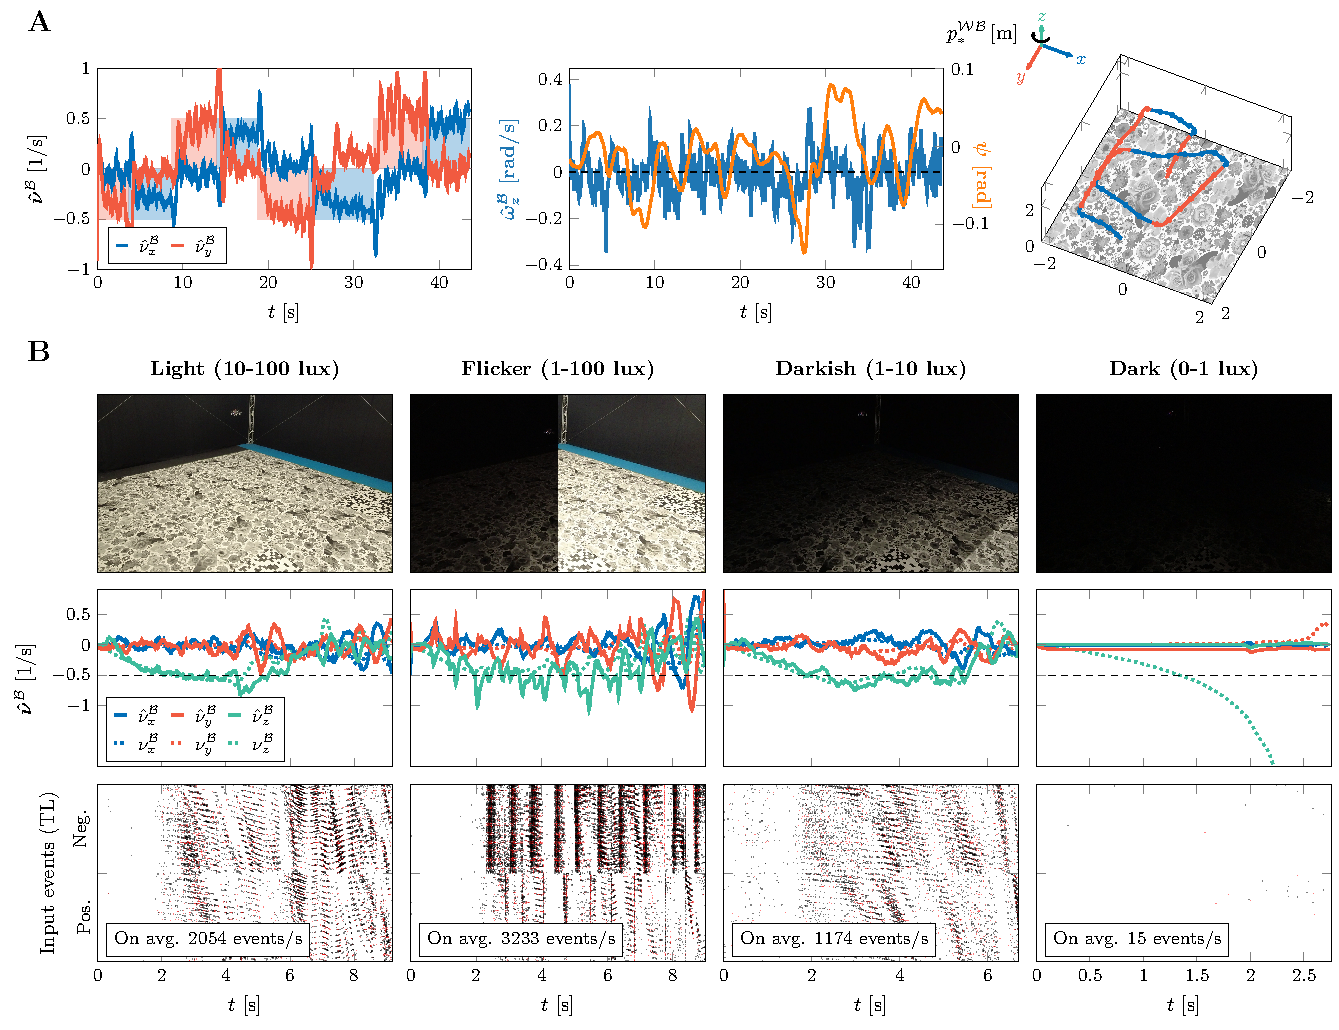
\includegraphics[width=\textwidth]{04_chapters/SR23/figures/fig9-snnspecial-results.pdf}
	\caption{Additional results with vision network and linear network controller. (\textit{A}) Alternating setpoints in X and Y (shaded areas) in order to fly a square. (\textit{B}) Landing experiments with different lighting conditions. While flickering lights lead to many more events, visual observable estimates (and hence control) only diverge when it is so dark that there are almost no events.}
	\label{fig:sr_snnspecial}
\end{figure}


\begin{figure}[!t]
	\centering
	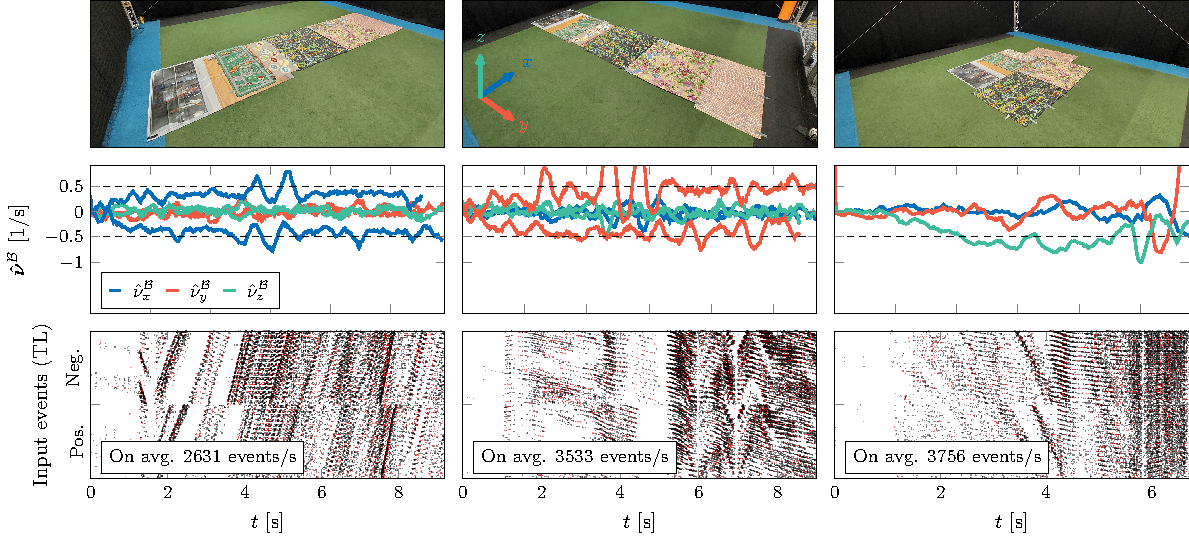
\includegraphics[width=\textwidth]{04_chapters/SR23/figures/fig8-snntexture-results.pdf}
	\caption{Results with vision network and linear network controller for various textures. Flight tests in X, Y and Z over variously textured mats show that the vision network is able to estimate optical flow regardless of texture. Input events are for the $\smash{\nu^\mathcal{B}_{\{x,y\},\mathrm{sp}} = 0.5}$~1/s and $\smash{\nu^\mathcal{B}_{z,\mathrm{sp}} = -0.5}$~1/s tests. Dashed lines show the nonzero setpoints in the motion axis.}
	\label{fig:sr_snntexture}
\end{figure}

\subsection{Benchmarking inference speed and energy consumption}

\begin{table*}[!t]
	\centering
	\resizebox{\textwidth}{!}{%
		\begin{tabular}{@{}lrrrrrrrr@{}}
			\thickhline
			\thickhline
			&  Seq.   & Static [W] & Dynamic [W] & Idle [W] & Running [W] & Delta [W] & inf/s & mJ/inf \\ \midrule
			Nahuku 32 (empty)                      & any    & 0.86      & 0.04       & 0.90    & 0.90       & 4\,e-3     & 60496 & 71\,e-6      \\ \midrule
			\multirow{3}{*}{Nahuku 32: SNN} & slow   & 0.90      & 0.05       & 0.94    & 0.95       & 12\,e-3     & 1637  & 7\,e-3      \\
			& medium & 0.90      & 0.04       & 0.94    & 0.95       & 8\,e-3     & 411   & 21\,e-3     \\
			& fast   & 0.90      & 0.04       & 0.94    & 0.95       & 7\,e-3     & 274   & 27\,e-3     \\ \midrule
			\multirow{3}{*}{Jetson Nano: SNN (5W)}      & slow   & -          & -           & 1.05  & 2.23       & 1.18     & 14     & 86.11 \\
			& medium & -          & -           & 1.03   & 2.25       & 1.22     & 14     & 85.58 \\
			& fast   & -          & -           & 1.03    & 2.24       & 1.21     & 14     & 86.19 \\ \midrule
			\multirow{3}{*}{Jetson Nano: SNN (10W)}     & slow   & -          & -           &  1.04   & 2.98       & 1.93     & 26     & 75.25 \\
			& medium & -          & -           &  1.06   & 2.98       & 1.92     & 26     & 75.35 \\
			& fast   & -          & -           &  1.04   & 2.99       & 1.95     & 25     & 76.52 \\ \midrule
			\multirow{3}{*}{Jetson Nano: ANN (5W)}      & slow   & -          & -           & 1.05  & 2.66       & 1.61     & 59     & 27.46 \\
			& medium & -          & -           & 1.07   & 2.64       & 1.57     & 56     & 27.91 \\
			& fast   & -          & -           & 1.06    & 2.64       & 1.58     & 57     & 27.52 \\ \midrule
			\multirow{3}{*}{Jetson Nano: ANN (10W)}     & slow   & -          & -           &  1.04   & 3.30       & 2.27     & 83     & 27.36 \\
			& medium & -          & -           &  1.07   & 3.33       & 2.26     & 80     & 28.09 \\
			& fast   & -          & -           &  1.07   & 3.30       & 2.23     & 80     & 27.80 \\ 
			\thickhline
			\thickhline
		\end{tabular}
	}
    \caption{Approximate energy and power characteristics for various devices on three sequences: slow, medium and fast. On average, slow has 28.6 events/inf, medium has 106.9 events/inf, and fast has 186.6 events/inf. Delta power is the difference between idle and running (total) power, and was used to compute energy per inference. Dynamic power is the power needed for switching and short-circuiting, and static power is due to leakage; together they sum to running (total) power as well. Nahuku is a board with 32 Loihi chips (Kapoho Bay has 2). A Nahuku configuration where no spikes were sent and only chips and cores were allocated (no synapses) is included as `empty'. Jetson Nano has a low-power (5W) and high-power (10W) mode. One inference (inf) was the processing of one set of inputs by the network, resulting in an output or prediction. On Jetson Nano, we tested both our vision SNN as well as the comparable Conv-GRU ANN.}
	\label{tab:sr_energy}
\end{table*}

\tabref{tab:energy} shows a comparison in terms of power/energy and runtime between the Loihi neuromorphic processor and an NVIDIA Jetson Nano for running the vision network (both SNN as well as equivalent ANN) on sequences with varying amounts of motion and hence varying input event density. The SNN ran in hardware on Loihi and in software (PyTorch) on Jetson Nano. The tests for Loihi were performed on a Nahuku board, which contains 32 Loihi chips. We confirmed, insofar possible, that using two chips on Nahuku is representative of a Kapoho Bay (at least in terms of execution time), which is the two-chip form factor used on the drone. Still, neither of these benchmarks is completely representative of the tests performed in the real world: the benchmarks used data already loaded in memory, and therefore only quantified the processing by the network without any bottlenecks due to input/output (I/O) and preprocessing, whereas the flight tests involved streaming event data that was coming in and was being processed in an online fashion. This showed in Loihi's execution frequencies in \tabref{tab:energy}, which were well above the 200 inferences (with one inference being the processing of one set of inputs by the network) per second (inf/s) achieved during flight tests.

\tabref{tab:energy} shows the power when the processors were idle and when they were running the networks. Because Jetson Nano does not provide static and dynamic power components, we compared the difference between idle and running power, and used that to compute energy per inference. A main observation is that the Nahuku 32 board consumed 0.95~W when running the SNN, whereas Jetson Nano consumed $\sim$2.98~W when running in 10W mode. This is a difference of a factor $\sim $3.1$\times$. Most of the energy expenditure of Loihi consisted of idle power. \tabref{tab:energy} also shows the difference between the idle power and the power when running the network (`Delta'). When only considering this extra power required for the inference of the network, Loihi outperformed Jetson Nano by three to four orders of magnitude, depending on the sequence. Hence, any possible reduction of the idle power would substantially affect the neuromorphic chip's energy efficiency advantages over other chips. 

Moreover, Loihi provided a one to two orders of magnitude improvement in execution frequency. Furthermore, the benefits of neuromorphic processing show in Loihi's increasing execution frequency as event sparsity increased (from fast to slow motion sequences).
Because a GPU like Jetson Nano is not optimized to simulate SNNs, we also ran an equivalent ANN (Conv-GRU with downsampling, corner crop ROI and event limiting from \tabref{tab:sr_AEEchanges}). The increased inference speed for the ANN on Jetson Nano confirms that this is indeed a more suitable architecture for GPUs. Nonetheless, although energy consumption per inference has decreased compared to running the SNN on Jetson Nano, energy efficiency and inference speed still did not come close to those of the SNN on Loihi.

\section{Conclusion}

We presented a fully neuromorphic vision-to-control pipeline for controlling a flying drone. Specifically, we trained a spiking neural network that takes in raw event-based camera data and produces low-level control commands. Real-world experiments demonstrated a successful sim-to-real transfer: the drone can accurately follow various ego-motion setpoints, performing hovering, landing, and lateral maneuvers\textemdash even under constant yaw rate. 

Our study confirms the potential of a fully neuromorphic vision-to-control pipeline by running on board with an execution frequency of 200~Hz. Moreover, the chip spends 0.95~W, out of which 0.94~W is idle power and only 7-12~mW is used for inference. Hence, reducing the idle power can lead to substantial energy gains. 

A major question is whether the energy gain of neuromorphic processing will make a difference on a system level even if future neuromorphic chips weigh in the order of grams and will have a negligible idle power. Compared to the power required for hovering, 277~W, a difference of a few watts (see \tabref{tab:energy}) may seem like a small difference. However, on flying robots, such small differences can have substantial effects \cite{boroujerdian2018mavbench}. A heavier, more power-consuming computing unit does not only require more power from the battery, but it also needs to be lifted in the air. This requires a bigger battery and possibly bigger motors that themselves also have to be lifted. Moreover, as argued in \cite{boroujerdian2018mavbench}, a lower latency, as attained with neuromorphic processing, allows for faster flight. This in turn leads to drones accomplishing their missions with less flight time. Still, the main point is not necessarily what you gain on a $\sim$1-kilogram drone if you switch from a conventional embedded GPU to a lightweight neuromorphic processor (which is not negligible), but that neuromorphic processing will enable many more networks to run on such larger drones and even enable deep neural networks on much lighter platforms that cannot even carry an embedded GPU. An example of the latter are 30-gram flapping wing drones, which use $\sim$6~W to fly\cite{karasek2018tailless}. 

A particularly promising avenue to autonomous flight of such tiny drones is to make the entire drone sensing, processing, and actuation pipeline neuromorphic, from its accelerometer sensors to the processor and motors, allowing for sparse and event-driven/asynchronous computation all the way through. Because such hardware is currently not available, we have limited ourselves to the vision-to-control pipeline, ending at thrust and attitude commands.

Until then, advancements could come from improved I/O bandwidth and interfacing options for the neuromorphic processor and event camera. The current processor is limited to host boards with an x86 architecture (preventing other potentially lighter but equally performant architectures from being used), and can only be connected directly via AER to a specific model of event-based camera (this is of course also a limitation on the part of the available event cameras). Although the former is limiting for all works implementing neuromorphic hardware on constrained systems like drones, the latter is especially relevant to our advanced use case, where we reached the limits of the number of spikes that can be sent to and received from the neuromorphic processor at the desired high execution frequency of 200~Hz. To achieve this frequency, we had to limit the number of events per input window to 90 per image corner ROI, and limit ourselves to a linear network controller, which avoids having to send additional input spikes that encode the ego-motion setpoint and attitude. Improved interfacing could allow for more extensive vision processing and more complex spiking neuron control networks. This could make the vision-based ego-motion estimation more robust and considerably increase the control performance\textemdash even if spiking neural network controllers currently perform worse than common PID controllers \cite{stagsted2020event,stroobants2022design}. Please note that as long as both the vision and control networks still use a learned encoding and decoding the proposed split-and-merge strategy would still work (see Materials and Methods). 
Ultimately, further gains in terms of efficiency might be obtained by moving from digital neuromorphic processors to mixed-signal hardware, but this will pose even larger development and deployment challenges given the noise sensitivity of such hardware \cite{sandamirskaya2022neuromorphic,frenkel2023bottomup}.

Despite the above-mentioned limitations, the current work presents a substantial step towards neuromorphic sensing and processing for drones. The results are encouraging, because they show that neuromorphic sensing and processing may bring deep neural networks within reach of small autonomous robots. In time this may allow them to approach the agility, versatility and robustness of small animals such as flying insects.

\section*{Supplementary material}
\vspace{10pt}
%\begin{itemize}
%	\setlength\itemsep{0.5em}
%	\item Video playlist of the approach: \textbf{TODO}
%%	\item Project code: \textbf{TODO}
%\end{itemize}

\newlist{mylist_sr}{itemize}{1}
\setlist[mylist_sr]{label=\hspace{0pt}}
\newcommand\itemonesr{\item \qrcode[height=0.4in]{https://www.youtube.com/playlist?list=PL_KSX9GOn2P-pyEODPVIb6PXfjr4BXuqH}}

\begin{mylist_sr}[leftmargin=*, align=left, leftmargin=2em, itemindent=0pt, labelsep=0pt, labelwidth=2em]
	\itemonesr\quad Video playlist of the approach: \url{https://tinyurl.com/4edsypye}
\end{mylist_sr}
	\chapter{Conclusion}
\label{cha:conclusion}

\dropcap{I}{n} this concluding chapter, we revisit and address the research questions and problem statement presented in \chapref{cha:intro}, which have structured the work conducted throughout this dissertation. We then discuss the broader implications of our findings and the potential impact that they may have on the broader scientific research field. Finally, we explore several potential avenues for future research.

\section{Answers to research questions}

The first research question derived from our problem statement was formulated as follows:

\tcbset{colframe=black!60!, coltitle=white}
\begin{tcolorbox}
	\textbf{RQ1}: How can fast, autonomous flight through gates be achieved with frame-based perception and conventional processing in a GPS-denied environment?
\end{tcolorbox}

This question was addressed in \chapref{cha:fr} with the development of a robust and efficient vision-based navigation solution for autonomous drone racing. To enable fast and agile flight using conventional sensing and processing, a lightweight monocular pipeline was devised, focusing exclusively on gate information. This was achieved by leveraging the fact that the gates were the only objects in the environment whose approximate appearance, location, and orientation were known a priori. The first step in the proposed pipeline is to detect the corners of the next gate to be traversed according to the flight plan, in the image space. This is done by first segmenting gate pixels using an artificial neural network (ANN) and then searching for the corners in the resulting mask using a light active-vision algorithm. The corners that can be validated using the robot's prior expectations of the gate's appearance and geometry are then used to estimate the pose of the camera in the world frame with a perspective-n-point algorithm. These vision measurements are enhanced with model-based predictions through random sample consensus, resulting in the state estimates used to control the robot. To finalize, a risk-aware control strategy is employed to balance the trade-off between speed and safety. The proposed solution was validated in hardware-in-the-loop simulation and real-world experiments. 
In fact, it was benchmarked against other state-of-the-art visual-inertial navigation solutions in the first Artificial Intelligence Robotic Racing season in 2019, where it was the fastest and most robust approach in those conditions, with the runner-up team being (only) three seconds slower in the final race.
%In fact, it was benchmarked against other state-of-the-art visual-inertial navigation solutions in the first Artificial Intelligence Robotic Racing season in 2019, where it was the fastest and most robust approach in those conditions, with the runner-up team being (only) 25\% slower on average.
%In fact, it was benchmarked against other state-of-the-art visual-inertial navigation solutions in the first Artificial Intelligence Robotic Racing season in 2019, where it was the fastest and most robust in those conditions, where it demonstrated its superiority as the fastest and most robust approach to autonomous drone racing in those conditions. 
Significantly, this chapter highlights the importance of minimizing latency in the perception pipeline to achieve high-speed autonomous flight. Our solution prioritized real-time performance at the system's maximum operating frequency (i.e., 60 Hz) over the use of more complex and computationally expensive algorithms.

\begin{tcolorbox}
	\textbf{RQ2}: How can we leverage the knowledge of the inner working of event cameras to learn event-based frame reconstruction in a self-supervised fashion?
\end{tcolorbox}

This second research question was motivated by the limited adoption of event cameras in robotics, despite their numerous advantages. This limited adoption is primarily due to the lack of a mature algorithmic ecosystem capable of effectively utilizing the sparse and asynchronous nature of event camera output. In \chapref{cha:cvpr}, we addressed this question by proposing a novel self-supervised learning (SSL) framework for event-based frame reconstruction. Our proposed solution is based on the event generative model, which, under constant illumination, establishes a relationship between events, brightness, and optical flow. Specifically, we demonstrate that this model can be leveraged to learn to reconstruct brightness frames from the events without relying on ground-truth data, as long as the optical flow encoded in the events is known or can be estimated. To achieve this, we train ANNs to minimize the discrepancy between the input events and the model-based predictions. The effectiveness of our training pipeline was validated using multiple datasets, where our networks demonstrated performance comparable to the state-of-the-art methods, despite not having access to reference frames during the training process. Additionally, we addressed the task of event-based optical flow estimation within the SSL framework. Our approach utilized the concept of contrast maximization for motion compensation, allowing us to learn event-based optical flow directly from the input events. Furthermore, we proposed a lightweight neural network architecture for event-based optical flow, which achieved high-speed inference while maintaining a minimal decrease in performance.

\begin{tcolorbox}
	\textbf{RQ3}: How can a spiking neural network learn to develop event-based motion selectivity in an unsupervised fashion?
\end{tcolorbox}

This third research question, focusing on event-based optical flow estimation with spiking neural networks (SNNs), was addressed in \chapref{cha:tpami}. Here, we introduced the first SNN that develops selectivity to motion, including direction and speed, in an unsupervised manner from the input event stream. The success of our approach was facilitated by the development of several key components. Firstly, we proposed a spiking neuron model capable of effectively handling the rapidly varying input statistics of event cameras through pre-synaptic adaptation. Secondly, we formulated a novel version of the correlation-based spike-timing-dependent plasticity (STDP) rule, which differs from the existing state-of-the-art approaches by being inherently stable. And finally, we designed a convolutional SNN architecture that learns to perform hierarchical feature extraction. Specifically, it starts by extracting geometric features, followed by capturing their local motion using multi-synaptic connections with different temporal delays, and eventually inferring global motion estimates via spatial integration. The effectiveness of this approach was validated through experimentation using both synthetic and real event sequences. However, due to the absence of supervision, quantitative comparisons with the state-of-the-art methods posed challenges. As a result, we relied on extensive qualitative analysis to assess and compare the performance of our approach. Most significantly, this chapter highlights the potential of SNNs to perform low-latency, event-based optical flow estimation. %Instead of having to accumulate events in the input representations, our approach allows for the processing of events nearly as they are generated by the sensor, with the integration of spatiotemporal information happening within the model itself.

\begin{tcolorbox}
	\textbf{RQ4}: How can low-latency, event-based optical flow be learned in a self-supervised fashion with spiking neural networks?
\end{tcolorbox}

This fourth research question, driven by the limitations of unsupervised learning, was addressed in \chapreftwo{cha:neurips}{cha:iccv}. In \chapref{cha:neurips}, we presented the first set of deep SNNs to successfully solve the problem of event-based optical flow estimation. To accomplish this, we reformulated the state-of-the-art training pipeline for ANNs (i.e., the aforementioned contrast maximization) to significantly reduce the time windows presented to the networks. Additionally, we refined the SSL loss function to enhance its convexity. Prior to training with our framework, we augmented various ANN architectures from literature with explicit and/or implicit recurrency, alongside the incorporation of the spiking behavior. Extensive quantitative and qualitative evaluations were conducted using multiple datasets. Our results not only confirm the efficacy of our training pipeline, but also demonstrate that the proposed set of recurrent ANNs and SNNs perform comparably to the state-of-the-art self-supervised methods.

Despite the significant accomplishments of \chapref{cha:neurips}, the proposed training pipeline assumes linear motion of events within the timeframe of their loss function, limiting its ability to accurately capture the true trajectory of scene points over time. To overcome this, \chapref{cha:iccv} introduces a reformulated pipeline that addresses the scalability to high inference frequencies while accurately capturing the true trajectory of scene points. An iterative event warping module and a multi-timescale loss function are the main additions to the pipeline. The former unlocks a novel multi-reference loss function that improves the accuracy of the predicted optical flow, while the latter enhances the robustness of the training process. The effectiveness of this new approach was validated using multiple datasets, where our models demonstrated superior performance compared to both the self-supervised and model-based baselines, surpassing them by significant margins. Please note that, although this reformulation of the training pipeline was validated with ANNs, it is extrapolable to SNNs as well.

\begin{tcolorbox}
	\textbf{RQ5}: How can a spiking neural network be trained in a self-supervised fashion to perform event-based optical flow estimation while running on a neuromorphic processor in the control loop of an autonomous flying robot?
\end{tcolorbox}

This fifth and last research question was tackled in \chapref{cha:sr}, where we introduced the groundbreaking concept of a fully neuromorphic vision-to-control pipeline for controlling a freely flying robot. The experimental setup involved equipping the robot with a downward-facing event camera, which captured data from a static planar surface, and a specialized neuromorphic processor. The latter was used to run a compact SNN that was trained to process high-dimensional raw event-camera data and output low-level control actions. This allowed for autonomous vision-based ego-motion estimation and control at approximately 200 Hz, spending only 27 $\mu$J per network inference. The proposed learning setup effectively addresses the challenge of slow and inaccurate simulation of event-based data, as it allows for the independent training of vision and control. While the vision part of the network is trained using an adapted version of the self-supervised pipelines from \chapreftwo{cha:neurips}{cha:iccv}, the control policy is learned through evolution in simulation without the need to simulate events. Real-world experiments were conducted, wherein the event camera and neuromorphic processor were integrated into the control loop of the flying robot. The results showcased the effectiveness of our approach, as the robot accurately followed various ego-motion setpoints and successfully performed hovering, landing, lateral maneuvers, and even constant yaw rate control.

The answer to this final research question, which builds upon the contributions of the previous chapters, also serves as the answer to our initial problem statement, which was formulated as follows:

\tcbset{colframe=black!90!, coltitle=white}
\begin{tcolorbox}
	\textbf{Problem Statement}: How can optical-flow-based autonomous navigation be realized with an event-based camera and a neuromorphic processor in the control loop of a flying robot?
\end{tcolorbox}

Our studies demonstrate the benefits of incorporating neuromorphic technology into the vision-based state estimation pipeline of autonomous flying robots, particularly in terms of latency and power consumption. The results obtained from our experiments are highly encouraging and suggest that the integration of neuromorphic sensing and processing could make deep neural networks more accessible for small autonomous robots (and other edge devices with limited resources). This advancement has the potential to enhance the agility, versatility, and robustness of these robots, bringing them closer to the capabilities exhibited by flying insects.

% \tcbset{colframe=black!90!, coltitle=white}
% \begin{tcolorbox}
	% 	\textbf{Driving Research Question}: How can neuromorphic perception and processing be incorporated into the vision-based, state-estimation pipeline of an autonomous flying robot?
	% \end{tcolorbox}

\section{Discussion}

The pursuit of incorporating neuromorphic technology into the control loop of autonomous flying robots has been the driving force behind the research presented in this dissertation. In this section, we delve into the main challenges encountered during this journey and the lessons we have gleaned along the way. Additionally, we shed light on the wider implications of our findings and the potential impact they can have on the broader scientific research field.

\subsection*{Efficient intelligence for flying robots}

Flying robots face inherent limitations due to their restricted payload capacity and power budget. Throughout our research, we have recognized the critical significance of developing efficient perception and processing pipelines to enable the autonomy of these robots. This theme has been at the core of our work, driving our exploration and innovations. In \chapref{cha:fr}, we developed a vision-based pipeline specifically tailored for autonomous drone racing with frame-based cameras. To ensure fast, agile, and robust flight, we leveraged classical (lightweight) algorithms wherever possible, while ANNs were used selectively where needed. Our research then shifted to exploring event-based cameras and SNNs as alternatives to conventional sensing and processing in \chapreffour{cha:cvpr}{cha:tpami}{cha:neurips}{cha:iccv}. These chapters highlight the potential of neuromorphic computing to achieve low-latency, low-power vision-based perception for robotics. Finally, in \chapref{cha:sr}, we demonstrated the feasibility of a fully neuromorphic vision-based pipeline for controlling a freely flying robot. This solution, which is characterized by an energy consumption in the order of microjoules and a latency of milliseconds, represents a significant step towards developing efficient intelligence for flying robots, as it shows that heavy processing can be realized on-board with only a fraction of the power needed to fly.  

\subsection*{Low-latency processing of event data with SNNs}

The event-camera literature has primarily focused on the use of stateless ANNs to process the data, with only a limited number of studies exploring the use of SNNs in often less complicated tasks. In this dissertation, we argue that to realize the full potential of event cameras and achieve low-latency and low-power solutions, stateful SNNs should process the incoming events nearly as they are generated by the sensor, with no accumulation in between. To support this claim, we have demonstrated the training of architecturally-complex SNNs for real-world, large-scale problems, specifically event-based optical flow estimation. In \chapref{cha:tpami}, we approached the problem from an unsupervised learning perspective using STDP to train the SNNs, while in \chapreftwo{cha:neurips}{cha:iccv}, we explored the self-supervised learning paradigm by employing new formulations of contrast maximization for motion compensation. In both approaches, we shortened the time windows presented to the networks and removed the temporal information from the input representations, approximating the way in which SNNs would receive events directly from the camera. This approach, which promotes the integration of spatiotemporal information within the models themselves through their internal dynamics, was then employed in \chapref{cha:sr} to realize the fully neuromorphic autonomous flight of a robot. Note that this idea has already sparked significant interest in the event-based optical flow literature, and several subsequent works have followed our findings \cite{ding2022spatio, ponghiran2022event, wu2022lightweight}, as they can potentially lead to lightweight solutions that are also robust to large pixel displacements.

\subsection*{Training SNNs with and without supervision}

In this dissertation, we tackled the problem of training SNNs for event-based optical flow estimation from two different learning perspectives: unsupervised and self-supervised. In \chapref{cha:tpami}, our focus was on unsupervised learning using the STDP rule, which adjusts the synaptic weights based on the temporal correlation between pre- and postsynaptic spikes. Despite the simplicity of this local learning rule, we successfully solved the task at hand by leveraging our knowledge of optical flow and the characteristics of event cameras to design an SNN capable of developing motion selectivity using this learning rule. However, the lack of supervision in STDP presents challenges. Firstly, it is difficult to directly benchmark our approach against the state-of-the-art since the learned features have limited controllability (i.e., we cannot specify what the network should learn). Secondly, careful fine-tuning of hyperparameters such as firing thresholds, decays, and synaptic delays is required to maintain a balanced network activity. On the other hand, the SSL paradigm explored in \chaprefthree{cha:neurips}{cha:iccv}{cha:sr} involves defining a loss function to be minimized during training, using the well-known backpropagation (through time) algorithm. This approach, once compensated for the non-differentiability of the spiking activation function \cite{neftciSurrogateGradientLearning2019, zenkeRemarkableRobustnessSurrogate2021}, enables us to leverage the vast array of tools and techniques developed for training ANNs. In these chapters, we demonstrated the effectiveness of this approach by training SNNs capable of estimating event-based optical flow with accuracy levels comparable to those of their ANN counterparts, and with the added benefit of being able to run on a neuromorphic processor. Note that the findings from our investigations on estimating event-based optical flow with SNNs have gotten the attention of the broader research community, as evidenced by the numerous follow-up works \cite{lee2020spike, vigneron2020critical, chaney2021self, barbier2021spike, liu2021event, parameshwaraSpikeMSDeepSpiking2021, she2021speed, peveri2021cortically, che2022differentiable, di2022kraken, yu2022improving, kosta2022adaptive, chamand2022self, zou2023event, negi2023best, iturbe2023nimbleai}.

\section{Outlook}

In this section, we explore several potential avenues for future research, which we believe can build upon the findings presented in this dissertation.

\subsection*{Toward per-event processing with SNNs}

One of the key insights from our research is that to fully harness the potential of event-based solutions, SNNs need to be trained to process incoming events nearly instantaneously as they are generated by the sensor. However, achieving this per-event processing approach is more complex than it might appear. There are two main challenges associated with this goal. Firstly, SNNs are recurrent networks with intricate internal dynamics. When the simulation timestep is decreased to enable per-event processing, the training process becomes significantly slower, and the memory requirements increase drastically if training with backpropagation through time (BPTT). BPTT, which has been shown in this dissertation to be a robust and effective gradient-based learning rule for SNNs, relies on accessing the network's internal states from previous timesteps to perform credit assignment over time. Consequently, these states need to be stored in memory throughout the BPTT process, which adds to the memory requirements. Secondly, as the simulation timestep decreases, the sparsity of the input increases. This means that there are fewer events occurring within each timestep, making it more challenging to extract meaningful patterns from the input data. We believe that these challenges could be addressed in multiple ways. One approach is to explore alternative learning rules that do not require the unrolling of networks in the backward pass, such as forward propagation through time \cite{yin2023accurate} or the forward-forward algorithm \cite{hinton2022forward}. These rules can reduce memory requirements and alleviate the computational burden of training SNNs. Additionally, leveraging the sparsity of SNNs and employing sparse computations during simulation can help reduce memory usage and increase inference speed. Techniques and frameworks that support sparse computations, such as the sparse module in PyTorch\footnote{See torch.sparse at \url{https://pytorch.org/docs/stable/sparse.html} (in beta at the time of writing this document).}, can be utilized for optimization. Lastly, another avenue of exploration is the use of more complex recurrent units, including potentially gated units, to enhance the ability of SNNs to extract meaningful patterns from sparse input data.

\subsection*{Robustifying unsupervised learning}

Unsupervised learning opens the door to backpropagation-free online learning in SNNs. However, an observation from our research is that while unsupervised learning rules can be effective in tasks where prior knowledge can be utilized in the network design, their applicability becomes limited when such knowledge is unavailable or cannot be incorporated into the architecture. For instance, in \chapref{cha:tpami}, we successfully trained an SNN to develop motion selectivity using STDP with a hierarchical architecture that enabled motion information to be discernible as clusters of spatiotemporal patterns. However, unsupervised learning may face challenges solving other tasks. To address this limitation and enhance the controllability of the learning process, we believe that future research on unsupervised learning for SNNs should focus on meta-learning, i.e., learning to learn. Specifically, we propose exploring the learning of the parameters of local learning rules, such as STDP, through either self-supervised or pure supervised approaches. By enabling the network to optimize its online learning rule in an offline training phase according to the needs of the task at hand, there is potential to enhance the robustness and deployability of SNNs. It is worth noting that some neuromorphic processors, such as Intel's Loihi \cite{davies2018loihi, orchard2021efficient}, already offer support for online learning through customizable local learning rules.

\subsection*{The future of neuromorphic flying robotics}

One of the primary contributions of this dissertation is the successful demonstration of a neuromorphic vision-to-control pipeline for controlling a freely flying robot with minimal latency and power consumption. This achievement represents a significant step forward in the field of event-based cameras and SNNs, and it marks the beginning of a long journey towards the development of fully neuromorphic, small (flying) robots. The development of such robots, surpassing the capabilities of their counterparts equipped with conventional sensors and processors, holds great promise for the future. However, to realize this vision, several challenges need to be addressed, both in terms of hardware and software. On the hardware side, a significant advancement could come from improving input/output (I/O) bandwidth in the processors. Enhancing the I/O capabilities can facilitate efficient data transfer between event-based sensors and neuromorphic processors, enabling faster and more seamless processing. Additionally, considerations for small form factors and low power consumption are essential for both the sensors and processors. Furthermore, there is potential for further efficiency gains by transitioning to analog neuromorphic processors, but this will pose even larger challenges in terms of their development and deployment. Regarding software, we reiterate the importance of per-event processing with SNNs, the need for scalable training pipelines and more complex recurrent units, and the potential of meta-learning. Once these challenges in hardware and software are overcome, the journey towards fully neuromorphic robots will gain significant momentum, enabling advancements in various areas of robotics and paving the way for a new era of intelligent and efficient machines.

	% \appendix
	
	\thumbfalse
	%%%%%%%%%%%%%%%%%%%%%%%%%
	
	\chapter*{References}
\addcontentsline{toc}{chapter}{References}
\setheader{References}

\begingroup
\renewcommand{\section}[2]{}%
\bibliographystyle{unsrt}
\bibliography{dissertation}
\endgroup

	\chapter*{Acknowledgments}
\addcontentsline{toc}{chapter}{Acknowledgments}
\setheader{Acknowledgments}

\dropcap{O}{ver} the course of my academic journey, there was a comic vignette by Reza Farazmand that played out like a little whisper of reassurance in the form of a mouse, saying, ``\textit{Everything is going according to plan}.'' And what was this plan, you might ask? ``\textit{Hope it all works out}.'' Little did I know, this seemingly light-hearted mantra would resonate with profound truth throughout my Ph.D.\ pursuit. 

\begin{figure}[!h]
	\centering
	\includegraphics[width=0.75\textwidth]{06_acks/plan.png}
	\caption*{``The Plan''. Picture credit: Reza Farazmand, author of Poorly Drawn Lines.}
	\label{fig:reza}
\end{figure}

As I stand here at the conclusion of this challenging yet rewarding chapter of my life, I am profoundly aware that the successful outcome was not solely due to my personal dedication and optimism that everything would work out in the end. It is clear to me that a lot of people played vital roles in this achievement, and I owe them my most sincere gratitude. This journey, with all its accomplishments, simply would not have been possible without their unwavering support and guidance.

I want to start by extending a heartfelt thank you to Guido and Christophe, my supervisory team, for the invaluable opportunity they have given me. Back in 2015, you warmly welcomed me into the MAVLab, making my decision to relocate to The Netherlands and all that it entailed truly worthwhile. Through the trust you placed in me, I was fortunate to live countless unique experiences, from an internship at Georgia Tech to participating in (and winning, \textit{yay!}) the AlphaPilot/AIRR competition. I am aware that I might not have been the easiest student to supervise, owing to my stubbornness and sometimes overly critical attitude, but I felt your confidence in me was always firm, and this allowed me to push even further. Thank you for your support both professionally and personally throughout this journey. It was an honor learning from and working with you.

To co-authors who later became friends, thank you for making my Ph.D.\ journey more fulfilling and enjoyable. Kirk, you were there from the very beginning of my time at the MAVLab, first as a supervisor and then as a colleague. You have been particularly influential during this phase of my life, and I cannot thank you enough for your invaluable contributions to my work and for facilitating my transition into Sony. Yingfu and Nilay, thank you for being my family at work. Your constant support and dedication, positiveness, and willingness to share perspectives from diverse backgrounds have enriched my understanding and broadened my horizons in ways I could have never imagined. Simply put, thank you. Jesse, Stein, and Julien, thank you for the transformative influence you had on the second half of my Ph.D. Your commitment, creativity, engaging discussions, and openness to entertain my, at times, unstructured ideas have been instrumental, and for that, I am truly grateful. I am confident that there are bright futures awaiting each of you, and I eagerly anticipate being a part of them.

I would also like to extend my appreciation to all the members of the MAVLab and C\&S who actively promote and maintain an inclusive and friendly work environment that fosters scientific advancements. Your dedication to creating such an environment has had a positive impact on my academic journey and the experiences of many others. In particular, thanks to Diana, Mario, Tom, Sven, Kimberly, Matěj, and many others who have been a part of this, whether they were here for a while or have moved on. Thank you for sharing the challenges and joys of our personal lives and academic endeavors.

During my time as a Ph.D.\ candidate, I was also fortunate to join Sony Europe for an internship. I would like to extend my gratitude to Oliver Erdler and Guido for making it possible, and to my colleagues Kirk, Diederik, Valentina, Vincent, and Manuel for making this experience both valuable and enjoyable. Having this break halfway through my Ph.D. allowed me to acquire valuable insights and skills that enriched my research journey and enabled me to better shape my professional career. For that, I am truly grateful.

It goes without saying that I hold deep appreciation for my friends outside university. I understand that at times, I can be somewhat distant, both physically and emotionally, but your support and understanding have meant the world to me. Thank you for always being there, whether through in-person interactions or via videogames. It is with you that I can truly find moments of disconnection.

Last but most definitely not least, quiero dar las gracias a mi familia por su apoyo incondicional a lo largo de mi vida, incluso en los momentos en los que mi ambici\'on nos ha distanciado m\'as de lo deseado. Pap\'a y Mam\'a, gracias por vuestra generosidad. Vuestro esfuerzo y sacrificio constante durante todos estos a\~nos ha hecho que, tanto Jes\'us como yo, hayamos crecido con amor, respeto y educaci\'on, además de con acceso a innumerables oportunidades. Sois nuestro ejemplo a seguir y siempre os estaremos agradecidos. Jes\'us, creciste siendo el peque\~no de dos hermanos, siguiendo muchos de mis pasos. Ir\'onicamente, ahora eres t\'u el que act\'ua como referente para m\'i en muchos aspectos. Gracias. Me siento muy afortunado de ser tu hermano, y siempre voy a estar aqu\'i para lo que necesites. Clara, es dif\'icil poner en palabras lo importante que eres para m\'i. Simplemente, gracias por darle equilibrio a mi vida y por cuidarme. Te quiero y admiro profundamente. Espero poder compensar en los pr\'oximos a\~nos todos los sacrificios que has hecho por m\'i y por este doctorado, el cual estoy orgulloso de poder compartir hoy contigo. Por \'ultimo, gracias de todo coraz\'on a mis abuelos/as, t\'ios/as (incluyendo, por descontado, a los presidentes de Komory's Club) y primos/as. Todos hab\'eis contribuido de una forma u otra, pero siempre positivamente, a que hoy pueda estar donde estoy. A todos, os quiero mucho.\newpage

As I close this chapter and step into new beginnings, I carry not only the knowledge and skills I've gained, but also the understanding that having a supportive community can truly transform one's journey. The mouse's simple but strangely profound mantra now reflects the gratitude I hold for each individual who played a part in making sure that, in the end, everything did work out.

\begin{flushright}
{\makeatletter\itshape
    Fede \\
    Delft, November 2023
\makeatother}
\end{flushright}

	\chapter*{Curriculum Vit\ae}
\addcontentsline{toc}{chapter}{Curriculum Vit\ae}
\setheader{Curriculum Vit\ae}

%% Print the full name of the author.
\makeatletter
\authors{\@firstname\ {\titleshape\@lastname}}
\makeatother

\noindent
\begin{longtable}{p{.225\textwidth} p{.70\textwidth}}
    01/04/1993 & Born in Katwijk, The Netherlands
\end{longtable}

\section*{Education}
\vspace{-10pt}
\noindent
\begin{longtable}{p{.225\textwidth} p{.70\textwidth}}
\end{longtable}
\vspace{-14pt}
\begin{longtable}{p{.225\textwidth} p{.70\textwidth}}
\end{longtable}
\vspace{-14pt}
\begin{longtable}{p{.225\textwidth} p{.70\textwidth}}
\end{longtable}
\vspace{-14pt}
\begin{longtable}{p{.225\textwidth} p{.70\textwidth}}
\end{longtable}

\section*{Experience}
\vspace{-10pt}
\noindent
\begin{longtable}{p{.225\textwidth} p{.70\textwidth}}
\end{longtable}
\vspace{-14pt}
\begin{longtable}{p{.225\textwidth} p{.70\textwidth}}
\end{longtable}
\vspace{-14pt}
\newpage
\begin{longtable}{p{.225\textwidth} p{.70\textwidth}}
\end{longtable}

\section*{Awards}
\vspace{-10pt}
\noindent
\begin{longtable}{p{.225\textwidth} p{.70\textwidth}}
\end{longtable}
\vspace{-14pt}
\begin{longtable}{p{.225\textwidth} p{.70\textwidth}}
\end{longtable}

	\chapter*{List of Publications}
\addcontentsline{toc}{chapter}{List of Publications}
\setheader{List of Publications}
\label{publications}

\noindent
$\dagger$~~Equal contribution.\\
\faFileTextO~~Included in this thesis.
\section*{Journal Papers}
\vspace{5pt}
\begin{etaremune}{\small
\item[\faFileTextO~~\hspace{4pt}7.] \emph{\textbf{F.\ Paredes-Vall\'es$^\dagger$}, J.\ J.\ Hagenaars$^\dagger$, J.\ D.\ Dupeyroux$^\dagger$, S.\ Stroobants, Y.\ Xu, G.\ C.\ H.\ E.\ de Croon}: Fully neuromorphic vision and control for autonomous drone flight. Under review at Science Robotics. 2023.
\item[\faFileTextO~~\hspace{4pt}6.] \emph{C.\ De Wagter$^\dagger$, \textbf{F.\ Paredes-Vall\'es}$^\dagger$, N.\ Sheth$^\dagger$, G.\ C.\ H.\ E.\ de Croon}: The sensing state-estimation and control behind the winning entry to the 2019 Artificial Intelligence Robotic Racing competition. Field Robotics. 2022.
\item[\faFileTextO~~\hspace{4pt}5.] \emph{C.\ De Wagter$^\dagger$, \textbf{F.\ Paredes-Vall\'es}$^\dagger$, N.\ Sheth$^\dagger$, G.\ C.\ H.\ E.\ de Croon}: Learning fast in autonomous drone racing. Nature Machine Intelligence (NMI). 2021.
\item[\faFileTextO~~\hspace{4pt}4.] \emph{D.\ B.\ de Jong, \textbf{F.\ Paredes-Vall\'es}, G.\ C.\ H.\ E.\ de Croon}: How do neural networks estimate optical flow? A neuropsychology-inspired study. IEEE Transactions on Pattern Analysis and Machine Intelligence (TPAMI). 2021.
\item[3.] \emph{J.\ J.\ Hagenaars, \textbf{F.\ Paredes-Vall\'es}, G.\ C.\ H.\ E.\ de Croon}: Evolved neuromorphic control for high speed divergence-based landings of MAVs. IEEE Robotics and Automation Letters (RA-L). 2020.
\item[\faFileTextO~~\hspace{4pt}2.] \emph{\textbf{F.\ Paredes-Vall\'es}, K.\ Y.\ W.\ Scheper, G.\ C.\ H.\ E.\ de Croon}: Unsupervised learning of a hierarchical spiking neural network for optical flow estimation: From events to global motion perception. IEEE Transactions on Pattern Analysis and Machine Intelligence (TPAMI). 2019.
\item[1.] \emph{S.\ Garc\'ia-Nieto, J.\ Velasco-Carrau, \textbf{F.\ Paredes-Vall\'es}, J.\ V.\ Salcedo, R. Simarro}: Motion equations and attitude control in the vertical flight of a VTOL bi-rotor UAV. Electronics. 2019.
}\end{etaremune}

\section*{Conference Papers}
\vspace{5pt}

\begin{etaremune}{\small
		\item[8.] \emph{Y.\ Wu, \textbf{F.\ Paredes-Vall\'es}, G.\ C.\ H.\ E.\ de Croon}: Lightweight event-based optical flow estimation via iterative deblurring. Under review at IEEE International Conference on Robotics and Automation (ICRA). 2024.
		\item[\faFileTextO~~\hspace{4pt}7.] \emph{\textbf{F.\ Paredes-Vall\'es}, K.\ Y.\ W.\ Scheper, C.\ De Wagter, G.\ C.\ H.\ E.\ de Croon}: Taming contrast maximization for learning sequential, low-latency, event-based optical flow. IEEE International Conference on Computer Vision (ICCV). 2023.
		\item[\faFileTextO~~\hspace{4pt}6.] \emph{R.\ J.\ Bouwmeester, \textbf{F.\ Paredes-Vall\'es}, G.\ C.\ H.\ E.\ de Croon}: NanoFlowNet: Real-time dense optical flow on a nano quadcopter. IEEE International Conference on Robotics and Automation (ICRA). 2023.
		\item[\faFileTextO~~\hspace{4pt}5.] \emph{J.\ J.\ Hagenaars$^\dagger$, \textbf{F.\ Paredes-Vall\'es}$^\dagger$, G.\ C.\ H.\ E.\ de Croon}: Self-supervised learning of event-based optical flow with spiking neural networks. Advances in Neural Information Processing Systems (NeurIPS). 2021.
		\item[4.] \emph{J.\ D.\ Dupeyroux, J.\ J.\ Hagenaars, \textbf{F.\ Paredes-Vall\'es}, G.\ C.\ H.\ E.\ de Croon}: Neuromorphic control for optic-flow-based landing of MAVs using the Loihi processor. IEEE International Conference on Robotics and Automation (ICRA). 2021.
		\item[\faFileTextO~~\hspace{4pt}3.] \emph{\textbf{F.\ Paredes-Vall\'es}, G.\ C.\ H.\ E.\ de Croon}: Back to event basics: Self-supervised learning of image reconstruction for event cameras via photometric constancy. IEEE/CVF Conference on Computer Vision and Pattern Recognition (CVPR). 2021.
		\item[2.] \emph{J.\ J.\ Hagenaars, \textbf{F.\ Paredes-Vall\'es}, G.\ C.\ H.\ E.\ de Croon}: Evolved neuromorphic control for high speed divergence-based landings of MAVs. IEEE/RSJ International Conference on Intelligent Robots and Systems (IROS). 2020.
		\item[1.] \emph{\textbf{F.\ Paredes-Vall\'es}, D.\ P.\ Magree, E.\ N.\ Johnson}: Direct feature correspondence in vision-aided inertial navigation for unmanned aerial vehicles. International Conference on Unmanned Aircraft Systems (ICUAS). 2017.
}\end{etaremune}
	
	\newpage
	\thispagestyle{empty}
	\phantom{blabla}
	\newpage
	
	\newpage
	\thispagestyle{empty}
	\phantom{blabla}
	\newpage
	
	% REMOVE FOR PRINTING
	% \setcounter{page}{0}\includepdf[pages=-]{coverback.pdf}  %%%%%%%%%%%%%%%%%%%%%%%%%%%%%%% CHECK
	% \setcounter{page}{0}\includepdf[pages=-]{propositions.pdf}  %%%%%%%%%%%%%%%%%%%%%%%%%%%%%%% CHECK
	
\end{document}

